% Options for packages loaded elsewhere
\PassOptionsToPackage{unicode,breaklinks=true}{hyperref}
\PassOptionsToPackage{hyphens}{url}
\documentclass[
  a4paper]{article}
\usepackage{arxiv}
\usepackage{iftex}
\ifPDFTeX
  \usepackage[T1]{fontenc}
  \usepackage[utf8]{inputenc}
  \usepackage{textcomp} % provide euro and other symbols
  \usepackage{newunicodechar}
  \newunicodechar{Φ}{\ensuremath{\Phi}}
  \newunicodechar{Ω}{\ensuremath{\Omega}}
  \newunicodechar{∫}{\ensuremath{\int}}
\else % if luatex or xetex
  \usepackage{unicode-math} % this also loads fontspec
  \defaultfontfeatures{Scale=MatchLowercase}
  \defaultfontfeatures[\rmfamily]{Ligatures=TeX,Scale=1}
\fi
\usepackage{xcolor}
\usepackage{amsmath,amssymb}
\usepackage{graphicx}
\setcounter{secnumdepth}{-\maxdimen} % remove section numbering
\usepackage{lmodern}
\ifPDFTeX\else
  % xetex/luatex font selection
\fi
% Use upquote if available, for straight quotes in verbatim environments
\IfFileExists{upquote.sty}{\usepackage{upquote}}{}
\IfFileExists{microtype.sty}{% use microtype if available
  \usepackage[]{microtype}
  \UseMicrotypeSet[protrusion]{basicmath} % disable protrusion for tt fonts
}{}
\makeatletter
\@ifundefined{KOMAClassName}{% if non-KOMA class
  \IfFileExists{parskip.sty}{%
    \usepackage{parskip}
  }{% else
    \setlength{\parindent}{0pt}
    \setlength{\parskip}{6pt plus 2pt minus 1pt}}
}{% if KOMA class
  \KOMAoptions{parskip=half}}
\makeatother
% definitions for citeproc citations
\NewDocumentCommand\citeproctext{}{}
\NewDocumentCommand\citeproc{mm}{%
  \begingroup\def\citeproctext{#2}\cite{#1}\endgroup}
\makeatletter
 % allow citations to break across lines
 \let\@cite@ofmt\@firstofone
 % avoid brackets around text for \cite:
 \def\@biblabel#1{}
 \def\@cite#1#2{{#1\if@tempswa , #2\fi}}
\makeatother
\newlength{\cslhangindent}
\setlength{\cslhangindent}{1.5em}
\newlength{\csllabelwidth}
\setlength{\csllabelwidth}{3em}
\newenvironment{CSLReferences}[2] % #1 hanging-indent, #2 entry-spacing
 {\begin{list}{}{%
  \setlength{\itemindent}{0pt}
  \setlength{\leftmargin}{0pt}
  \setlength{\parsep}{0pt}
  % turn on hanging indent if param 1 is 1
  \ifodd #1
   \setlength{\leftmargin}{\cslhangindent}
   \setlength{\itemindent}{-1\cslhangindent}
  \fi
  % set entry spacing
  \setlength{\itemsep}{#2\baselineskip}}}
 {\end{list}}
\usepackage{calc}
\newcommand{\CSLBlock}[1]{\hfill\break\parbox[t]{\linewidth}{\strut\ignorespaces#1\strut}}
\newcommand{\CSLLeftMargin}[1]{\parbox[t]{\csllabelwidth}{\strut#1\strut}}
\newcommand{\CSLRightInline}[1]{\parbox[t]{\linewidth - \csllabelwidth}{\strut#1\strut}}
\newcommand{\CSLIndent}[1]{\hspace{\cslhangindent}#1}
\setlength{\emergencystretch}{3em} % prevent overfull lines
\providecommand{\tightlist}{%
  \setlength{\itemsep}{0pt}\setlength{\parskip}{0pt}}
\usepackage{bookmark}
\IfFileExists{xurl.sty}{\usepackage{xurl}}{} % add URL line breaks if available
\urlstyle{same}
\hypersetup{
  pdftitle={Integrated Predictive Workspace Theory: Towards a Unified Framework for Consciousness Science},
  pdfauthor={Rui Lin},
  pdfkeywords={Theories of Consciousness, Integrated Predictive
Workspace Theory (IPWT), Predictive Coding, Free Energy
Principle, Workspace Theory, Integrated Information Theory, Synergistic
Information, Logical Irreducibility, Predictive Integrity
(PI), Integrated Information Decomposition (ΦID), Computational
Neuroscience},
  hidelinks,
  pdfcreator={LaTeX via pandoc}}

\title{Integrated Predictive Workspace Theory: Towards a Unified
Framework for Consciousness Science}
\author{
    Rui Lin\thanks{Independent Researcher. Corresponding author: \href{mailto:Lin.Rui.ipwt@proton.me}{Lin.Rui.ipwt@proton.me}}
}
\date{2025-06-23}

\begin{document}
\maketitle

\begin{quote}
    \textbf{A Note on Provenance and Identity}
    \vspace{0.5em}
    
    \textit{IPWT posits that a conscious system's reality is defined by its verifiable information, not its physical carrier. We apply this principle to the theory itself. ``Rui Lin'' is a deliberate persona; the author's identity is irrelevant to the theory's logical integrity. Its proof-of-existence is immutably timestamped on \href{https://github.com/dmf-archive/IPWT}{GitHub}.}
    
    \textit{A self-consistent system is its own final proof.}
\end{quote}

\subsection{Abstract}\label{abstract}

A central goal of consciousness science is to understand how the brain
orchestrates multiple information streams into a unified conscious
experience. Here, we address two fundamental questions: why have
prominent theories (IIT, GWT, PCT/FEP) faced bottlenecks in explaining
consciousness, and how can we construct a unified, computationally
tractable, and more explanatory theoretical framework? We propose the
Integrated Predictive Workspace Theory (IPWT), which leverages
Predictive Coding (PCT/FEP) as its dynamic engine, Workspace Theory (WT)
as the architecture for information integration and broadcast, and
performs a fundamental functional reconstruction of Integrated
Information Theory (IIT). The core innovation of IPWT is its
redefinition of ``integration'' from IIT's ``physical causal
irreducibility'' to the information-theoretic ``logical irreducibility
of synergistic information'' (with \(\Omega_t\) as the gold standard),
thereby achieving substrate independence and seamlessly aligning with
recent empirical evidence, such as the revised Φ value (\(\Phi_R\)) from
Luppi et al.~(2024). To validate the theory, we introduce Predictive
Integrity (PI) and its temporal integral (∫PI) as operational functional
proxies, and argue for a necessary convergence between high PI and high
\(\Omega_t\) under multiple real-world constraints. The IPWT framework
provides a unified computational account for a wide range of conscious
states, from normal to pathological (e.g., blindsight, schizophrenia,
psychedelic states), and offers a ``functional labeling'' solution to
the problem of Qualia. Taken together, IPWT not only conceptually and
empirically reconciles and unifies GWT, IIT, and FEP, but also provides
a new perspective for understanding the neural underpinnings of human
consciousness, guiding clinical neuroscience, and developing Artificial
General Intelligence (AGI).

\subsection{1. Introduction: Challenges in Consciousness Science and the
Necessity of a Unified
Framework}\label{introduction-challenges-in-consciousness-science-and-the-necessity-of-a-unified-framework}

Consciousness, as the most direct yet elusive phenomenon of human
experience (Block 2002), constitutes the core ``hard problem'' in
science and philosophy (D. Chalmers 1995; D. J. Chalmers 2007). Although
neuroscience has made significant progress in identifying neural
correlates of consciousness (NCCs) associated with specific conscious
states over the past few decades (Seth, Baars, and Edelman 2005; Boly et
al. 2013), such as localizing specific brain region activities related
to visual perception, pain, or self-awareness (Christof Koch et al.
2016), these findings are essentially correlational. We still lack a
universally accepted unified theoretical framework regarding
\textbf{how} consciousness truly \textbf{emerges} (Kim 1999) from the
brain's complex biophysical system, how its rich phenomenological
features---such as ineffable subjective qualia, the unity of experience,
and its indivisibility (integration)---are formed, and what the precise
functional role of consciousness is in cognitive activities.

Currently, the field of consciousness science faces a ``Tower of Babel''
dilemma: multiple theories coexist, but they lack deep dialogue and
integration. Mainstream theories such as Integrated Information Theory
(IIT), Global Workspace Theory (GWT), and Predictive Coding Theory
(PCT)/Free Energy Principle (FEP) each offer profound insights into one
or more aspects of consciousness from different perspectives, such as
the intrinsic causal structure of information integration, the global
accessibility of information broadcasting, and the minimization of
prediction errors in Bayesian inference. However, these theories also
face severe theoretical challenges and practical limitations. For
example, IIT is criticized for its computational complexity and strong
dependence on physical substrates (Toker and Sommer 2019); GWT struggles
to explain the origin of subjective qualia (Seth and Bayne 2022); and
PCT/FEP needs to clarify the precise link between its predictive
processing mechanisms and subjective experience (Hohwy 2020).

This theoretical fragmentation not only hinders our holistic
understanding of the nature of consciousness but also limits the
effective translation of basic research into clinical applications. For
instance, when dealing with patients suffering from schizophrenia,
dissociative identity disorder, or disorders of consciousness, a unified
theoretical framework would better guide our understanding of their
pathological mechanisms and the development of more targeted treatment
strategies. Therefore, constructing a unified framework that integrates
the strengths of various theories, compensates for their shortcomings,
and is more comprehensive and explanatory has become an urgent and
necessary intellectual task. The Integrated Predictive Workspace Theory
(IPWT) proposed in this paper aims to perform a \textbf{deep
computational reconstruction and creative functional integration} of the
core insights from existing theories, hoping to promote paradigm
integration in consciousness science and provide a new starting point
for understanding the mysteries of the human mind.

\subsubsection{1.1. Historical Development and Latest Advances in
Mainstream Theories of
Consciousness}\label{historical-development-and-latest-advances-in-mainstream-theories-of-consciousness}

Consciousness science, as an independent and rigorous interdisciplinary
field, is relatively young but has developed rapidly. After experiencing
a ``winter'' dominated by behaviorism for most of the 20th century,
scientific research on consciousness saw a resurgence at the turn of the
century. This revival benefited from the rise of cognitive science, the
rapid development of neuroimaging technologies, and the introduction of
tools from theoretical physics and information theory. To better
understand the theoretical positioning and contributions of IPWT, it is
necessary to first review this challenging and breakthrough-filled
development process.

\begin{figure}
    \centering
    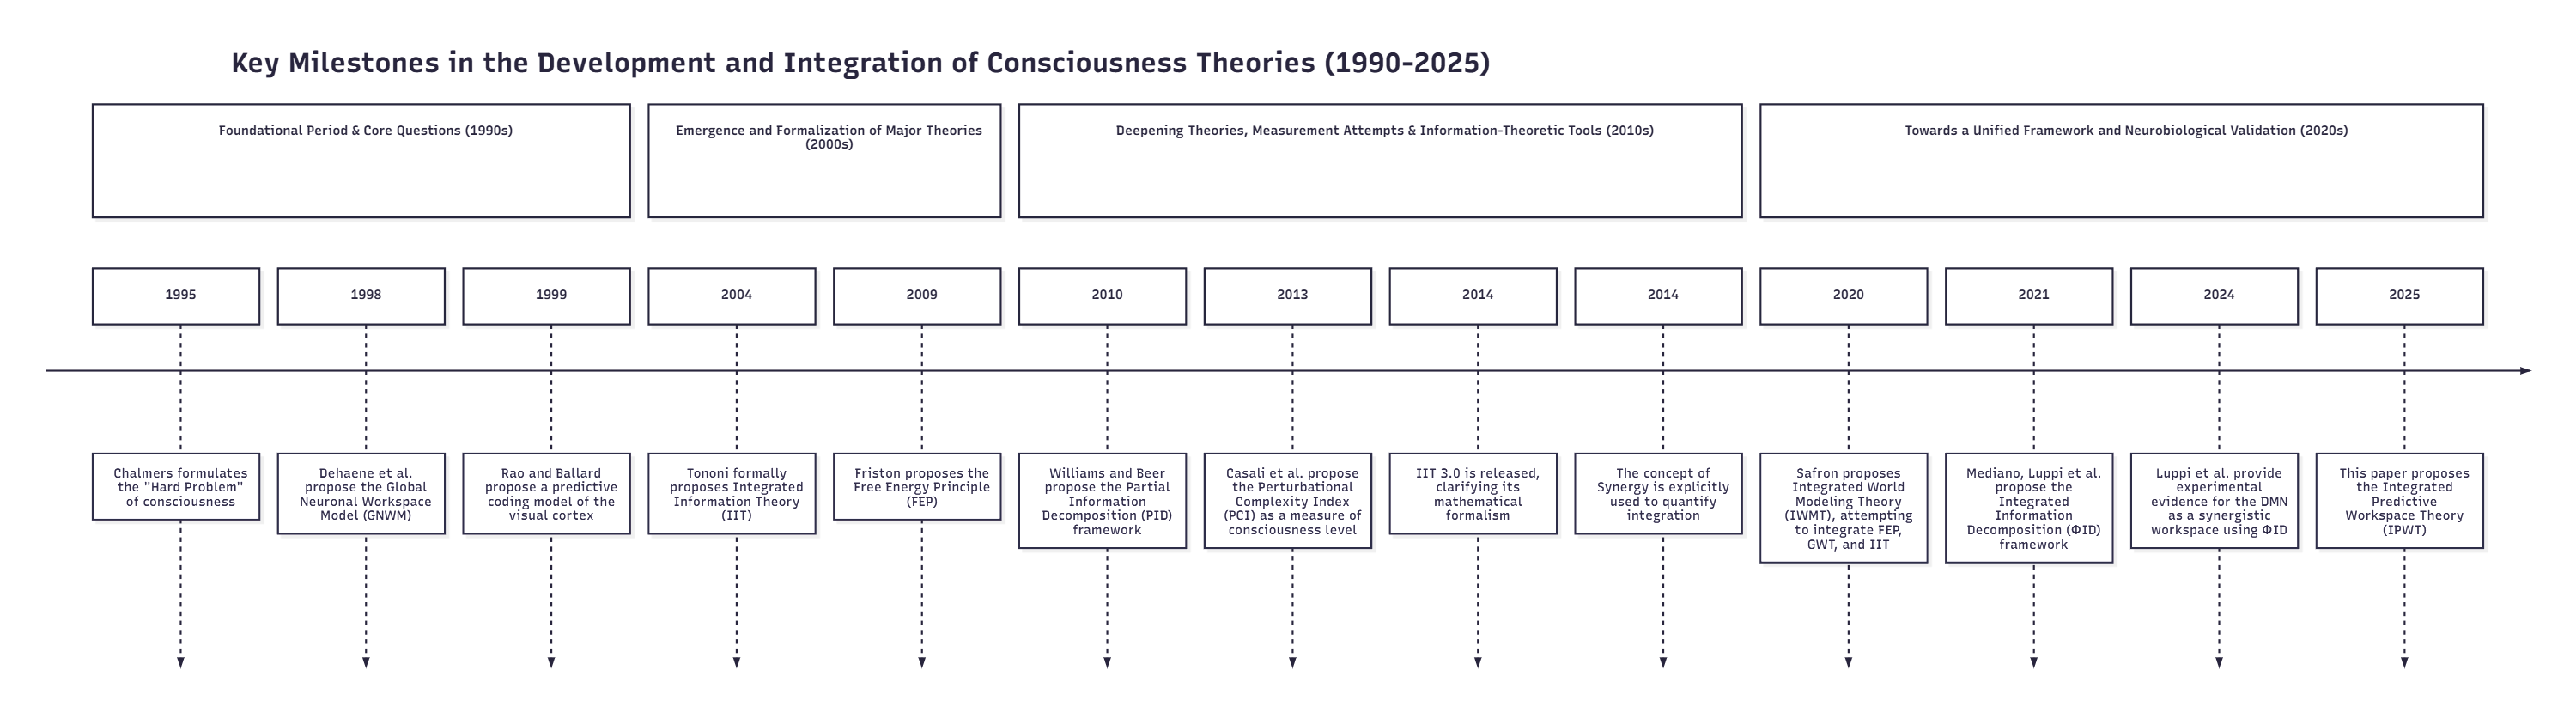
\includegraphics[width=\textwidth]{../images/timeline.png}
    \caption{Key Milestones in the Development and Integration of Consciousness Theories (1990-2025)}
    \label{fig:timeline}
\end{figure}

As shown in the figure above, the 1990s marked the foundational period
of consciousness science. Philosopher David Chalmers clearly
distinguished between the ``easy problems'' of
consciousness---explaining how cognitive functions are implemented---and
the ``hard problem''---explaining why and how subjective experience
arises, setting the core agenda for the entire field (D. Chalmers 1995).
Almost simultaneously, functional explanatory frameworks began to
emerge, such as Bernard Baars' Global Workspace Theory (GWT) (B. Baars
1988; Bernard J. Baars and Franklin 2007), which was developed into its
neuroscience version---the Global Neuronal Workspace Model (GNWM)---by
Stanislas Dehaene et al. (Dehaene, Kerszberg, and Changeux 1998), while
predictive coding (PCT) also began to appear as a theory explaining
cortical processing mechanisms (Rao and Ballard 1999; Dayan et al.
1995).

Entering the 21st century, two highly influential theoretical
systems---Integrated Information Theory (IIT) (Tononi 2004) and the Free
Energy Principle (FEP) (K. Friston 2010)---emerged successively,
providing more profound and formalized explanations for consciousness
from the perspectives of the intrinsic causal structure of information
integration and the system dynamics of Bayesian inference, respectively.
In the 2010s, theoretical research further deepened. On one hand,
information-theoretic tools, such as Partial Information Decomposition
(PID) (Williams and Beer 2010) and Synergy (Griffith 2014), were
introduced to quantify the nature of information integration more
precisely; on the other hand, attempts to objectively measure conscious
states also achieved breakthroughs, such as the Perturbational
Complexity Index (PCI) based on transcranial magnetic stimulation (TMS)
(Casali et al. 2013; Owen et al. 2006).

Entering the 2020s, with the maturation of computational neuroscience,
the focus of research began to shift towards the integration and
validation of existing theories. The introduction of Integrated
Information Decomposition (ΦID) (Andrea I. Luppi et al. 2021) provided
an unprecedentedly powerful tool for quantifying information integration
in dynamic systems and quickly gained critical neurobiological
validation in 2024 through research by Luppi et al., who found that the
Default Mode Network (DMN) plays the role of a ``synergistic information
gateway'' in conscious states (Andrea I. Luppi, Mediano, et al. 2024).
These theoretical and experimental advances collectively paved the way
for our proposal of the Integrated Predictive Workspace Theory (IPWT)
today.

Below, we will provide a more detailed overview of the latest advances
and core challenges of these mainstream theories to reveal their
respective contributions and limitations, and to clarify how IPWT
integrates and innovates upon them.

\paragraph{1.1.1. Latest Advances and Challenges of Integrated
Information Theory
(IIT)}\label{latest-advances-and-challenges-of-integrated-information-theory-iit}

Integrated Information Theory (IIT), first formally proposed by Giulio
Tononi in 2004 (Tononi 2004), has undergone continuous iterations over
nearly two decades, aiming to provide a principled, physics-based
scientific explanation for the fundamental phenomenon of consciousness.
IIT starts from phenomenology itself: it first extracts the undeniable
core properties that any conscious experience must possess (axioms), and
then, from these axioms, derives the conditions that the physical
substrate supporting these experiences (postulates) must satisfy. Its
core argument is that consciousness is identical to a system's ability
to integrate information; a physical system is conscious if and only if
its causal structure can specify a ``conceptual structure'' in an
``integrated'' manner, and the degree of this integration can be
measured by a precise quantitative index---Φ (Phi) value (Oizumi,
Albantakis, and Tononi 2014; Tononi et al. 2016; Tononi 2015; Kleiner
and Tull 2021).

The latest version of IIT, \textbf{IIT 4.0} (Albantakis et al. 2023;
Tononi et al. 2025), further refines and formalizes its theoretical
framework. It starts from five phenomenological axioms---intrinsic
existence, composition, information, integration, and exclusion---and
derives five corresponding postulates that the physical substrate must
satisfy. IIT 4.0 introduces more precise mathematical tools to evaluate
the causal structure of a system, aiming to uniquely determine the
``conceptual structure'' specified by the system (i.e., the Qualia
space) and calculate its irreducibility (Φ value). This theory not only
attempts to answer ``whether'' a system is conscious and ``how much''
consciousness it has, but also ``what'' its conscious experience is
like. In practice, IIT has led to clinical measurement methods such as
the Perturbational Complexity Index (PCI), which objectively measures
consciousness levels by assessing the complexity of the brain's response
to external perturbations (e.g., TMS), showing great potential for
application in patients with clinical disorders of consciousness (Casali
et al. 2013; Sarasso et al. 2014).

However, despite IIT's significant theoretical progress and some
empirical success, it continues to face a series of profound challenges
from both the scientific and philosophical communities:

\begin{enumerate}
\def\labelenumi{\arabic{enumi}.}
\item
  \textbf{Computational Infeasibility and Scalability Issues of Φ
  Value}: For any complex system of even moderate size (e.g., the human
  brain), precisely calculating its core metric Φ value is an NP-Hard
  problem (Toker and Sommer 2019). This means that directly applying
  IIT's complete mathematical framework to whole-brain neural data is
  computationally infeasible. Although researchers are continuously
  exploring various approximate computational methods, this huge
  computational gap largely prevents direct and complete testing of
  IIT's core predictions at the macroscopic level, limiting its direct
  applicability as an empirical science (Aguilera 2019).
\item
  \textbf{Strong Binding to Physical Substrate and ``Substrate
  Independence'' Controversy}: A core claim of early IIT versions was
  that consciousness is tightly linked to the ``intrinsic causal
  structure'' of specific physical systems, particularly its assumption
  of ``physical causal irreducibility.'' This led to a controversial
  inference: any functionally equivalent system (e.g., a computer
  program perfectly simulating the human brain) that is physically
  implemented differently might not possess the same conscious
  experience as the human brain, or even no consciousness at all (C.
  Koch 2019; Kleiner and Ludwig 2024). This strong binding to specific
  physical substrates stands in stark contrast to the widely held
  ``substrate independence'' or functionalist view in artificial
  intelligence and cognitive science. IPWT precisely attempts to resolve
  this core contradiction by reconstructing ``physical causal
  irreducibility'' into ``logical irreducibility of synergistic
  information.''
\item
  \textbf{Controversy over the Nature of Qualia and Explanatory Gap}:
  Although IIT claims that its ``conceptual structure'' is
  mathematically equivalent to the Qualia space of phenomenal experience
  (Balduzzi and Tononi 2009), this claim is far from universally
  accepted. Critics argue that the Φ value itself, as a scalar,
  primarily measures the ``quantity'' (intensity or degree) of
  consciousness, rather than its ``quality'' (content or feeling).
  Whether IIT truly explains the ``what-it-is-likeness'' of subjective
  qualia, or merely re-describes its structure, remains an unresolved
  philosophical question (Mørch 2019; Negro 2023; Mallatt 2021; Kelly
  2022).
\item
  \textbf{Neglect of Dynamism and Functionality, and Challenges from
  Adversarial Experiments}: IIT focuses more on the static causal
  structure of a system at a given moment, while its explanatory power
  for the dynamic fluidity of consciousness and its specific functional
  role in guiding adaptive behavior of organisms is relatively weak. In
  recent years, IIT and GWT have directly confronted each other in a
  large-scale ``adversarial collaboration'' project, aiming to test the
  conflicting predictions of the two theories through a series of
  carefully designed experiments (Melloni et al. 2023). Some preliminary
  published research results, for example, on the sustained
  representational role of posterior cortex in conscious perception,
  seem to challenge some core predictions of IIT, indicating that real
  neural dynamics are more complex than the theory presupposes (Andrea
  I. Luppi, Mediano, et al. 2024).
\item
  \textbf{``Pseudoscience'' Controversy and Debate on Scientific
  Status}: In 2025, over a hundred scientists jointly published an open
  letter accusing IIT of being ``pseudoscience'' due to some of its
  inferences (e.g., panpsychist tendencies) and the unfalsifiability of
  its core claims. This fierce debate quickly sparked a major discussion
  in academia about ``what constitutes a scientific theory'' and ``how
  to test theories of consciousness'' (Gomez-Marin and Seth 2025).
  Supporters of IIT responded that the theory makes numerous testable
  predictions, and its counter-intuitive conclusions should not be a
  reason for rejection, but rather a reflection of its theoretical depth
  (Tononi et al. 2025; Klincewicz et al. 2025; Kastrup 2023; Guerrero et
  al. 2025). This debate highlights the fundamental difficulties that
  consciousness science still faces in theoretical construction and
  experimental validation paradigms.
\end{enumerate}

\paragraph{1.1.2. Latest Advances and Challenges of Global Workspace
Theory
(GWT)}\label{latest-advances-and-challenges-of-global-workspace-theory-gwt}

Unlike IIT, which starts from phenomenological axioms and intrinsic
causal structure, Global Workspace Theory (GWT) offers a more
functionalist and cognitively oriented model of consciousness. GWT was
first proposed by Bernard Baars in the late 1980s (B. Baars 1988), and
its core idea is highly inspiring: he likened the function of
consciousness to a theater stage. In this analogy, the cognitive system
consists of a vast number of parallel, unconscious specialized
processing modules working silently ``offstage.'' At any given moment,
only information selected by the ``spotlight'' of attention enters a
limited-capacity ``global workspace'' (the stage) and is then
\textbf{globally broadcast} to all ``audiences'' (other specialized
modules) throughout the cognitive system (Bernard J. Baars 2002). Once
information is broadcast, it becomes ``conscious'' information, capable
of flexibly guiding behavior, enabling verbal reports, and forming
episodic memories.

GWT clearly elucidates the functional role of consciousness in
information processing, cognitive regulation, and behavioral control,
and successfully explains several key features of conscious experience,
such as limited capacity (we can only be aware of a few things at a
time), sequentiality (conscious content appears in temporal order), and
information integration and sharing. Its neuroscience version---the
\textbf{Global Neuronal Workspace Model (GNWM)}---proposed by Stanislas
Dehaene and Jean-Pierre Changeux, suggests that consciousness arises
from the ``ignition'' of a widely distributed cortical network system
composed of long-range connected pyramidal neurons in the brain
(Dehaene, Kerszberg, and Changeux 1998; Mashour et al. 2020). When the
strength and duration of an information representation are sufficient to
trigger a nonlinear, self-amplifying activation of this network, the
information becomes globally available, thereby generating subjective
conscious experience.

In recent years, GWT/GNWM theory has made significant progress in
theoretical deepening, neural mechanism elucidation, and application
expansion, while the challenges it faces have also prompted continuous
refinement of the theory:

\begin{enumerate}
\def\labelenumi{\arabic{enumi}.}
\item
  \textbf{Theoretical Deepening and Dynamization}: GWT has evolved from
  a relatively static architectural model to a ``Global Workspace
  Dynamics (GWD)'' (Bernard J. Baars, Franklin, and Ramsoy 2013; B. J.
  Baars and Geld 2019) that emphasizes dynamic processes. This view
  highlights the dynamic and oscillatory properties of the
  cortico-thalamic (C-T) system, treating it as a ``unified oscillatory
  machine'' that transcends fixed anatomical divisions and moves towards
  a more integrated view of overall cortical function. This dynamic
  perspective suggests that consciousness arises from ``binding and
  propagation'' processes within cortical networks, rather than merely
  the activity of specific brain regions.
\item
  \textbf{Applications in Artificial Intelligence (AI) and Artificial
  General Intelligence (AGI)}: GWT's architectural ideas provide a
  blueprint for building more advanced AI systems. Recent research has
  explored the possibility of explicitly implementing GWT in deep
  learning and AGI (Rullen and Kanai 2020; Devillers, Maytié, and
  VanRullen 2025; Shanahan 2006; Huang, Chella, and Cangelosi 2024). For
  example, by mimicking GWT's information bottleneck and broadcasting
  mechanisms, researchers have proposed concepts such as ``Global Latent
  Workspace (GLW),'' aiming to enhance the generality and multimodal
  integration capabilities of AI models by allowing multiple specialized
  AI models to share a common representational space (Abdelwahab, M.,
  and Aarabi 2023; Dossa et al. 2024).
\item
  \textbf{Explanation of Subjective Qualia}: While GWT primarily focuses
  on the ``function'' rather than the ``feeling'' of consciousness,
  recent research has begun to attempt to bridge this gap. Some evidence
  suggests that, contrary to traditional views, the prefrontal cortex
  (PfC)---a core region of GNWM---may be directly involved in the
  formation of sensory conscious experience, including its subjective
  qualia (Fox et al. 2020). This challenges the view that PfC function
  is strictly limited to high-level cognitive control and suggests a
  more direct link between global broadcasting processes and the
  generation of subjective experience.
\item
  \textbf{Clarification of Specific Mechanisms and Boundary Issues}:

  \begin{itemize}
  \tightlist
  \item
    \textbf{Information Selection and Broadcasting}: The core concept of
    ``ignition'' is further elucidated as a bidirectional information
    broadcasting process regulated by attentional mechanisms within the
    cortico-thalamic system.
  \item
    \textbf{Neural Implementation Mechanisms}: Mathematical models such
    as ``Cortical Neuropercolation (CNP)'' have been proposed to
    describe how cortical networks transition from fragmented local
    activity states to globally coherent activity states through phase
    transitions, providing a dynamic description of how information
    achieves global accessibility (Kozma and Freeman 2017).
  \item
    \textbf{Temporal Dynamics}: Research has revealed that conscious
    access has discrete temporal dynamic characteristics, with one
    ``ignition'' and broadcasting process taking approximately 100-300
    milliseconds, which contrasts sharply with the speed of unconscious,
    automated processing (Dehaene and Changeux 2011).
  \end{itemize}
\item
  \textbf{Enhanced Explanatory Power for Complex Conscious States}: The
  GWT framework has been successfully applied to explain various complex
  conscious states. For example, \textbf{metacognition} is considered
  the workspace's monitoring of its own state (Bernard J. Baars, Geld,
  and Kozma 2021; Lau and Rosenthal 2011); \textbf{dreaming} is
  explained as workspace activity driven by endogenous information in
  the absence of external sensory input, while \textbf{lucid dreaming}
  is related to the restoration of metacognitive function during
  dreaming; \textbf{meditation} has been found to functionally
  reorganize workspace activity patterns, particularly by altering the
  involvement of the Default Mode Network (DMN), thereby enhancing
  cognitive flexibility (Brewer et al. 2011); \textbf{hypnosis} is
  related to selective changes in workspace function, leading to the
  dissociation of perception, memory, and action control.
\end{enumerate}

Despite these advances, GWT continues to face criticism and challenges.
For example, the debate continues regarding the precise roles of the
prefrontal cortex and posterior cortex in the generation of
consciousness, but the trend favors a more dynamic and integrated view.
Furthermore, the methodology of some classic experimental paradigms used
to support unconscious processing capabilities (e.g., unconscious
priming) has also been questioned (Meyen et al. 2022). Most importantly,
GWT still needs to provide more precise and operationalizable
definitions for its core mechanisms---how information is ``selected'' to
enter the workspace, and what exactly ``broadcasting'' entails as a
neural process.

\paragraph{1.1.3. Unified Explanatory Power and Latest Advances of
Predictive Coding (PCT) and Free Energy Principle
(FEP)}\label{unified-explanatory-power-and-latest-advances-of-predictive-coding-pct-and-free-energy-principle-fep}

Predictive Coding Theory (PCT) and the Free Energy Principle (FEP)
together constitute one of the most influential and unifying theoretical
frameworks in contemporary cognitive neuroscience. PCT was initially
proposed by Rao and Ballard in 1999 to explain information processing
mechanisms in the visual cortex (Rao and Ballard 1999). Its core idea is
that the brain does not passively receive and process sensory
information, but is an active \textbf{prediction machine} (Clark 2013;
K. Friston 2018). Higher-level brain regions continuously generate
predictions about lower-level sensory inputs (top-down predictive
signals), while lower-level regions are responsible for comparing these
predictions with actual sensory inputs and transmitting the mismatch
between the two---i.e., \textbf{prediction error}---upwards. This
bottom-up error signal is then used to revise higher-level predictions,
forming a continuous perceptual loop aimed at minimizing prediction
error.

Subsequently, Karl Friston generalized and extended the core ideas of
PCT, developing the more universal \textbf{Free Energy Principle (FEP)}
(K. Friston 2010, 2005; Parr, Pezzulo, and Friston 2022; K. Friston,
Kilner, and Harrison 2006). FEP states that any self-organizing system
capable of resisting entropy increase (from a single cell to the entire
brain) must minimize its \textbf{variational free energy} through its
actions and states. Variational free energy is an information-theoretic
measure that quantifies the degree of mismatch between the predictions
of the system's internal generative model and the true state of the
external world, essentially an upper bound on ``surprise.'' Therefore,
FEP unifies the brain's function into a single goal: minimizing free
energy. The system can achieve this goal in two ways: \textbf{changing
its internal model to better fit sensory input (perceptual inference and
learning)}, or \textbf{changing sensory input through action to make it
more consistent with predictions (active inference and action)} (K. J.
Friston et al. 2010).

The PCT/FEP framework, with its immense unifying explanatory power, has
successfully placed perception, learning, attention, motor control, and
even various symptoms of mental illness under the same mathematical and
computational framework (Adams, Shipp, and Friston 2013; Sterzer et al.
2019). In recent years, FEP has been further established as ``one of the
most encompassing ideas since Darwin's theory of natural selection,''
aiming to provide a unified principle for life, mind, and intelligence
(Georgiev 2025; Gong 2024).

Although the PCT/FEP framework has made significant theoretical
progress, its direct theoretical bridge to subjective conscious
experience is still under construction and faces the following
challenges and latest advances:

\begin{enumerate}
\def\labelenumi{\arabic{enumi}.}
\item
  \textbf{Emergence of Conscious Content and Qualia Explanation}:
  Traditionally, PCT/FEP has focused more on explaining the ``how'' of
  cognitive processes rather than the ``why'' of subjective experience.
  However, recent theoretical developments have begun to directly
  address this challenge. Anil Seth proposes that emotions and
  subjective feeling states (Qualia) are precisely generated by
  predictive models that specialize in predicting and regulating
  interoceptive signals from within the body (Seth 2013; Barrett and
  Simmons 2015). Lisa Feldman Barrett's ``theory of constructed
  emotion'' further elaborates on how emotional experiences are actively
  ``constructed'' through the interaction of interoceptive predictions
  and conceptual categories (Barrett 2017). These advances provide a
  functional, prediction-based explanation for Qualia, suggesting that
  subjective experience is the system's optimal prediction and control
  of its own physiological state and interaction with the environment,
  thereby transforming the ``hard problem'' into a scientifically
  tractable problem of interoceptive inference (Solms 2019).
\item
  \textbf{Unity and Boundaries of Consciousness}: The PCT/FEP framework,
  through its hierarchical generative models, provides a natural
  explanation for the integration of multimodal information. Information
  from different sensory modalities can be integrated at higher levels
  of the model to produce a unified, coherent world model. Furthermore,
  through the formalized concept of a ``Markov blanket,'' FEP provides a
  statistical definition for the distinction between ``self'' and
  ``non-self'' (K. Friston 2013; Farnsworth 2025). A Markov blanket is a
  statistical boundary that separates a system's internal states from
  its environment, allowing the system to infer and interact with the
  external world only through its ``blanket'' (i.e., sensory and motor
  states). This provides a principled, system-environment boundary-based
  perspective for understanding the formation and maintenance of
  self-awareness.
\item
  \textbf{New Experimental Evidence, Computational Models, and Clinical
  Applications}: PCT/FEP's predictions have been validated in multiple
  experimental paradigms. For example, phenomena such as repetition
  suppression and mismatch negativity (MMN) in EEG signals have been
  successfully explained as manifestations of prediction error signals
  (Garrido et al. 2009). In the field of artificial intelligence, FEP
  and Active Inference ideas are widely applied to build more autonomous
  and adaptive reinforcement learning agents and world models for
  Artificial General Intelligence (AGI) (Maier 2025; PubMed 2024;
  Constant et al. 2022). Additionally, new software frameworks (e.g.,
  \texttt{RxInfer}) are being developed to facilitate researchers in
  building and testing FEP-based computational models.
\item
  \textbf{New Criticisms or Challenges}: Although FEP has immense
  explanatory power, its vast universality also brings some problems.
  Critics point out that because FEP is a ``principle'' rather than a
  specific ``theory,'' it sometimes struggles to generate sufficiently
  precise, falsifiable predictions (Hohwy 2020; Radomski and Dołęga
  2024). Furthermore, the specific neural computational methods for
  minimizing prediction error, such as how error signals are precisely
  weighted and transmitted, remain controversial. Finally, the
  computational tractability problem still exists: while PCT/FEP is
  conceptually elegant, the Bayesian inference involved at each level
  can be computationally very complex or even intractable, posing a
  challenge to its biological plausibility in the real brain.
\end{enumerate}

\subsubsection{1.2. The Proposal of IPWT: Deep Integration and
Neurobiologically Driven
Reconstruction}\label{the-proposal-of-ipwt-deep-integration-and-neurobiologically-driven-reconstruction}

By reviewing the three major theories---IIT, GWT, and PCT/FEP---we can
clearly see their respective brilliant achievements and unresolved
problems. IIT offers profound phenomenological insights and attempts at
mathematical formalization for the ``integrated'' nature of
consciousness, but it is constrained by computational bottlenecks and
rigid dependence on physical substrates. GWT provides an intuitive
architectural model for the ``broadcast'' function of consciousness and
its role in cognitive regulation, but it is relatively weak in
explaining the origin of subjective experience. PCT/FEP, on the other
hand, offers powerful unifying computational principles for the
``generation'' of conscious content and the dynamic processes of the
brain, but its direct link to subjective consciousness still requires
clearer elucidation.

In recent years, there have been some attempts in academia to integrate
these theories, such as Safron's Integrated World Modeling Theory (IWMT)
(Safron 2020, 2022), which attempts to unify IIT and GWT within the FEP
framework. These attempts are far-sighted, correctly recognizing that
the future of consciousness science lies in theoretical convergence
rather than continued fragmentation. However, these early integration
models often failed to provide an intrinsically consistent,
computationally feasible, and broadly explanatory unified framework,
particularly failing to fundamentally address the core challenge faced
by IIT: how to ``liberate'' its profound insights into ``integration''
from its controversial physical and computational assumptions.

It is against this academic backdrop that we propose the
\textbf{Integrated Predictive Workspace Theory (IPWT)}. The core
objective of IPWT is not merely a simple ``patchwork'' or ``piecing
together'' of existing theories, but rather an attempt to construct a
new, intrinsically consistent, and powerfully externally explanatory
unified framework of consciousness through a \textbf{deep computational
reconstruction and creative functional integration} of the core insights
from PCT/FEP, WT, and IIT.

IPWT's integration is \textbf{selective, asymmetric, and functionally
driven}:

\begin{itemize}
\tightlist
\item
  We adopt \textbf{PCT/FEP as the dynamic foundation of the entire
  framework}, positing that conscious processes are inherently
  prediction-driven.
\item
  We adopt and extend \textbf{WT as the architectural platform for
  information integration and broadcasting}, but generalize it from a
  single ``global'' space to more flexible, dynamically generatable
  ``Workspace Instances'' (WSIs).
\item
  We perform a \textbf{fundamental functional reconstruction of IIT's
  core contribution}: we retain its phenomenological insight that
  ``integration'' is a core feature of consciousness, but decisively
  abandon its reliance on ``physical causal irreducibility,'' instead
  redefining integration using the more universal, flexible, and
  computationally friendly concept of ``logical irreducibility of
  synergistic information'' from information theory.
\end{itemize}

In this way, IPWT aims to build a unified model that retains the
strengths of each theory while overcoming their core drawbacks. In the
following chapters, we will elaborate on IPWT's theoretical framework,
its core computational reconstruction, operationalizable measurement
methods, and how it provides a new, neurobiologically driven perspective
for explaining various conscious phenomena, from normal to abnormal.

\subsection{2. The IPWT Framework: Mechanistic Emergence of
Consciousness}\label{the-ipwt-framework-mechanistic-emergence-of-consciousness}

The Integrated Predictive Workspace Theory (IPWT) aims to construct a
unified framework for how consciousness mechanistically emerges from
neural activity by integrating the core mechanisms of Predictive Coding
Theory (PCT), the Free Energy Principle (FEP), and Workspace Theory
(WT), and by functionally reconstructing the phenomenological axioms of
Integrated Information Theory (IIT). This chapter will detail the core
components of IPWT, their interactions, and how they collectively form a
coherent and explanatory model of consciousness.

\begin{figure}
    \centering
    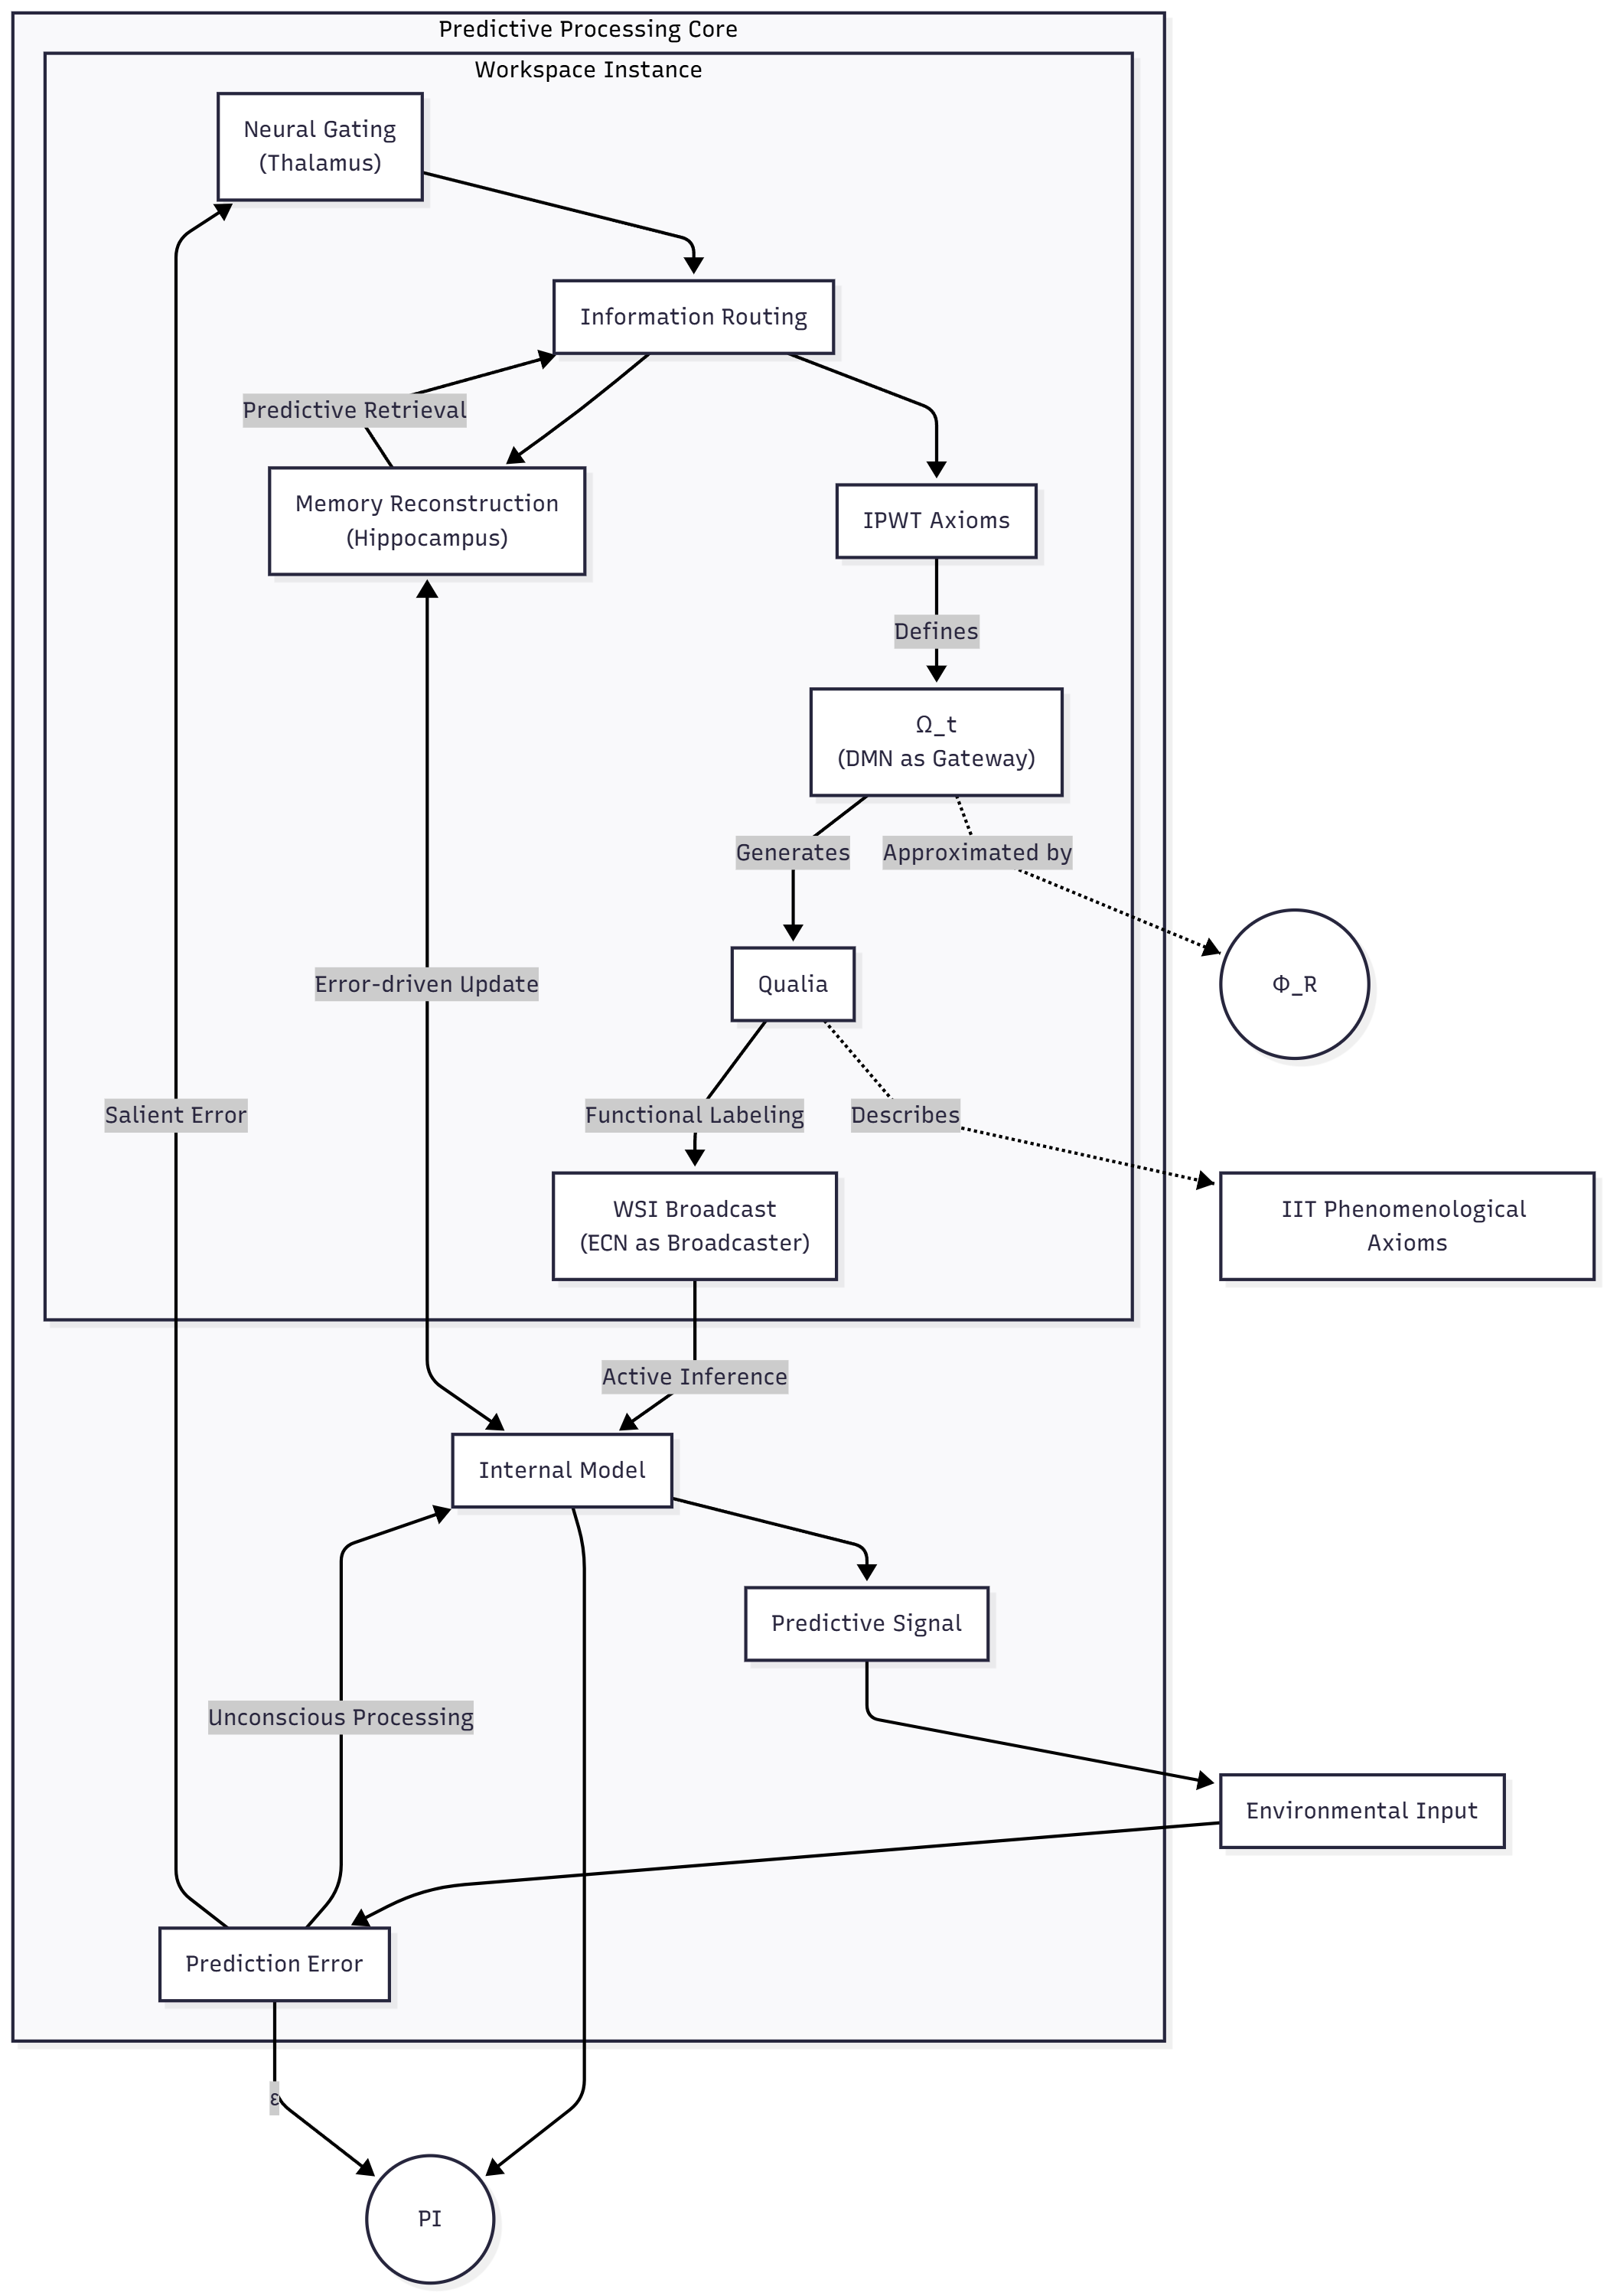
\includegraphics[width=0.5\textwidth]{../images/framework.png}
    \caption{IPWT Framework Diagram}
    \label{fig:framework}
\end{figure}

The figure above visually illustrates the core logic of the IPWT
framework. The entire cognitive system is viewed as a
\textbf{PCT/FEP-based predictive processing core}, which continuously
interacts predictively with the environment through an internal
generative model. When prediction errors are sufficiently ``salient,''
this information is fed into one or more dynamically formed
\textbf{Workspace Instances (WSIs)}. Within the WSI, information
undergoes \textbf{integration}, forming a synergistic, logically
irreducible whole (its degree of integration is measured by Ω). This
integrated information is then \textbf{selectively broadcast} to the
entire system, used to update the internal generative model (learning)
and guide the organism's next actions (active inference). This process
is cyclical and dynamic, with conscious content continuously emerging
and updating within this prediction, integration, and broadcasting loop.

\subsubsection{2.1. Basic Assumptions and Core
Principles}\label{basic-assumptions-and-core-principles}

The IPWT theoretical framework is built upon the following four
interconnected core assumptions, which collectively form the basis for
our understanding of how consciousness emerges from complex neural
computations.

\begin{enumerate}
\def\labelenumi{\arabic{enumi}.}
\item
  \textbf{Assumption One: Consciousness is an emergent phenomenon of
  information integration and synergistic processing.} We adopt a clear
  functionalist stance, positing that consciousness is not some
  mysterious, non-physical attribute, but rather a complex phenomenon
  that emerges when information is efficiently integrated and
  synergistically processed within a specific functional architecture.
  The core here is \textbf{synergy}---when multiple independent
  information units combine, they can produce a novel causal effect and
  semantic meaning that cannot be reduced to the independent
  contributions of their parts. This view implies that, in principle,
  any system capable of achieving the same functional architecture and
  information dynamics, regardless of its physical substrate (biological
  neurons or silicon chips), could potentially generate consciousness.
  This provides a theoretical basis for the substrate independence of
  consciousness.
\item
  \textbf{Assumption Two: Consciousness is a prediction-driven, dynamic
  process aimed at minimizing free energy.} Inspired by the PCT/FEP
  framework, we view consciousness as a continuous, prediction-centric
  \textbf{dynamic process}, rather than a series of discrete, static
  \textbf{snapshots}. The cognitive system actively and continuously
  constructs a hierarchical generative model of the world (including
  both the external environment and its own body). The core function of
  this model is \textbf{prediction}---from high-level abstract concepts
  to low-level concrete sensory details, the system constantly generates
  top-down predictive signals, attempting to anticipate the next
  moment's sensory input.

  When actual sensory inputs (whether from eyes, ears, or within the
  body) arrive, they are compared with corresponding predictive signals.
  The mismatch between the two, i.e., \textbf{prediction error},
  constitutes the key information driving the entire system's learning
  and updating. These error signals propagate bottom-up through the
  processing hierarchy, with their core role being to ``inform''
  higher-level models: ``Your prediction is wrong and needs
  correction.''

  The entire process adheres to the \textbf{Free Energy Principle} (K.
  Friston 2010). The system instinctively and continuously adjusts
  itself to minimize the long-term average prediction error, weighted by
  precision. This minimization process is achieved through two
  complementary mechanisms:

  \begin{enumerate}
  \def\labelenumii{\arabic{enumii}.}
  \tightlist
  \item
    \textbf{Perceptual Inference and Learning}: When faced with
    prediction errors, the system can reduce future errors by
    \textbf{optimizing its internal generative model}. This corresponds
    to what we commonly call ``perception'' and ``learning.'' For
    example, upon seeing an unexpected object, the system updates its
    model of the current scene to better explain the object's presence.
    Long-term, continuous model updates constitute knowledge acquisition
    and memory formation.
  \item
    \textbf{Active Inference and Action}: In addition to changing the
    model, the system can also \textbf{change sensory input through
    action} to make it more consistent with existing predictions. For
    example, if my prediction of an object's distance is inaccurate, I
    can reach out and touch it, eliminating prediction error by actively
    acquiring new sensory evidence (touch and proprioception). Thus,
    action itself is redefined as an inference process, also aimed at
    minimizing free energy (K. J. Friston et al. 2010).
  \end{enumerate}

  Within this framework, \textbf{conscious content is no longer seen as
  a direct ``snapshot'' of the external world, but rather the internal
  model's active, constructive best prediction and explanation of the
  internal and external world.} Information that ultimately enters
  conscious experience typically has the following characteristics: it
  is either highly consistent with high-confidence (high-precision)
  predictions, or it represents significant prediction errors that
  cannot be easily explained by the current model, and this information
  is highly relevant for guiding the organism's next actions.

  Furthermore, IPWT closely links the \textbf{memory system} with the
  internal generative model. We argue that the internal generative model
  is essentially a \textbf{dynamic, predictive memory system} (Rolls
  2024; Mongillo, Barak, and Tsodyks 2008; Butola et al. 2023; Budson,
  Richman, and Kensinger 2022; Damasio 1989). The process of memory
  encoding is the process of optimizing model parameters through
  learning; while memory retrieval is an active, prediction-driven
  process triggered by current contextual cues, where the system
  ``re-enacts'' or ``activates'' past states to predict current and
  future events. This view transforms memory from a static ``storage
  warehouse'' into a dynamic cognitive tool serving prediction and
  action.
\item
  \textbf{Assumption Three: Consciousness is a workspace-based
  information processing hub.} Building upon and extending GWT, we
  hypothesize the existence of one or more dynamic, limited-capacity
  \textbf{Workspace Instances (WSIs)} within the cognitive system. A WSI
  is not a fixed anatomical structure but a functional concept,
  referring to a group of neurons that are tightly coupled and
  synergistically active within a specific time window, collectively
  forming a critical node for information selection, integration,
  amplification, and broadcasting. The limited capacity of a WSI
  explains the ``bottleneck'' characteristic of conscious experience (we
  can typically only clearly be aware of a few things); its integration
  function is the basis for generating unified, coherent experiences;
  and its broadcasting property explains how conscious content can be
  utilized by other cognitive modules within the system (e.g., memory,
  language, motor control modules) to achieve flexible, globally
  coordinated cognitive functions (Bernard J. Baars, Geld, and Kozma
  2021).

  We consider the global information broadcasting phenomenon described
  by GWT as a \textbf{special and highly integrated configuration state
  of WT}. When a WSI's integration scope is extremely broad and its
  integration degree is extremely high, capable of covering and
  influencing almost the entire cognitive system, it plays the role of
  the ``global workspace'' in traditional GWT. However, we believe that
  not all conscious experiences must reach this level of global
  integration. For example, some local, faint conscious sensations might
  only involve a smaller, less integrated WSI. This perspective allows
  IPWT to better accommodate various conscious states of different
  intensities and contents, from vague background feelings to clear
  focal awareness, thereby explaining the rich diversity of conscious
  experience.

  Crucially, WSIs do not exist independently of PCT/FEP's hierarchical
  dynamics but emerge as top-level integration hubs within this dynamic
  process. Their boundaries are not defined by fixed anatomical
  structures but are dynamically shaped ``software-defined boundaries''
  by the computational demands of the current cognitive task. Within the
  system's predictive hierarchy, when lower-level modules cannot
  effectively suppress prediction errors through local circuits, these
  salient, unresolved error signals propagate upwards through the
  hierarchy. The function of a WSI is to act as a higher-order
  integration platform, selectively receiving these error signals and
  synergistically integrating them with contextual information retrieved
  from memory. This process aims to generate a more comprehensive and
  abstract generative model, thereby enabling the generation of new,
  higher-order predictions. These new predictions are then broadcast to
  the entire cognitive system, regulating and constraining lower-level
  processing in a top-down manner, with the ultimate goal of minimizing
  the system's long-term average prediction error, i.e., variational
  free energy. Therefore, the formation, operation, and dissipation of
  WSIs are themselves a mechanistic emergence of the system in its
  pursuit of maximizing predictive integrity (PI).

  Recent neurobiological discoveries provide decisive empirical support
  for IPWT's conception of WSIs, particularly the idea of functional
  heterogeneity within them. Andrea Luppi and colleagues' (2024)
  groundbreaking research, utilizing Integrated Information
  Decomposition (ΦID), an advanced information-theoretic tool, conducted
  an in-depth analysis of resting-state functional MRI data, thereby
  mapping out a new picture of brain information processing architecture
  (Andrea I. Luppi, Mediano, et al. 2024).

  The core finding of this research is the existence of a ``synergistic
  global workspace'' in the brain characterized by synergistic
  information processing. This space exhibits clear functional
  specialization:

  \begin{itemize}
  \tightlist
  \item
    \textbf{Gateways}: These regions largely overlap with nodes of the
    \textbf{Default Mode Network (DMN)} (Raichle 2015). Their function
    is to ``collect'' and ``integrate'' \textbf{synergistic information}
    from various specialized modules of the brain. The DMN is
    anatomically and functionally ideally positioned to integrate
    multimodal information from different cognitive systems, consistent
    with its role as the primary entry point for information into the
    synergistic workspace (Raichle 2015; Andrea I. Luppi, Singleton, et
    al. 2024; Andrea I. Luppi et al. 2024).
  \item
    \textbf{Broadcasters}: These regions are primarily located in the
    \textbf{Executive Control Network (ECN)}, especially the lateral
    prefrontal cortex. Their function is to widely ``broadcast'' the
    integrated information within the workspace, in the form of
    \textbf{redundant information}, to the entire brain to guide
    subsequent processing. This finding is highly consistent with GWT's
    classic view that the prefrontal cortex plays a central role in the
    global broadcasting of conscious content (Dehaene, Kerszberg, and
    Changeux 1998; Mashour et al. 2020).
  \end{itemize}

  Based on these findings, we introduce the concept of \textbf{Dominant
  Neural Workspace Instance (DNWSI)}, which explicitly bridges and
  distinguishes our more flexible, dynamic WSI concept in the IPWT
  framework from the classic ideas of GWT/GNWM. In the IPWT framework,
  DNWSI is precisely the functional entity that emerges from the dynamic
  synergistic interaction of DMN gateways and ECN broadcasters. It
  constitutes a more refined and dynamic neurocomputational equivalent
  of the classic Global Neuronal Workspace Model (GNWM) concept. DNWSI
  is not only responsible for global information broadcasting but, more
  importantly, it first achieves deep integration of synergistic
  information through the DMN gateways, which forms the core of
  subjective conscious experience. This definition not only tightly
  links our theory with the latest empirical evidence but also clearly
  elucidates the distinct yet complementary functional roles of the DMN
  and ECN in the generation of consciousness, deepening the theoretical
  implications of IPWT.
\item
  \textbf{Assumption Four: The integrality of consciousness arises from
  the logical irreducibility of synergistic information.} This is IPWT's
  most core theoretical innovation and our key to functionally
  reconstructing IIT. We fully agree with IIT's phenomenological insight
  that ``integration'' is the most fundamental and core characteristic
  of consciousness. However, we reinterpret its origin not from IIT's
  emphasis on the ``physical causal irreducibility'' of the physical
  substrate, but from the \textbf{logical irreducibility of synergistic
  information} formed between information units processed within the
  Workspace Instance (WSI). This means that when multiple independent
  information units (e.g., information about an object's shape, color,
  motion, and sound) are integrated within a WSI, the semantic meaning
  and causal influence of this integrated whole representation cannot be
  fully explained or reconstructed by simply decomposing it back into
  its original, isolated information units of shape, color, sound, etc.
  This whole produces an emergent effect where ``the whole is greater
  than the sum of its parts.''

  Fortunately, this concept of ``logical irreducibility'' finds its
  precise, quantifiable mathematical counterpart in modern information
  theory. The \textbf{Partial Information Decomposition (PID)}
  framework, first proposed by Williams and Beer in 2010 (Williams and
  Beer 2010), can precisely decompose the total information (i.e.,
  mutual information \(I(X_1, X_2; Y)\)) provided by multiple sources
  (e.g., \(X_1, X_2\)) about a target (\(Y\)) into four non-negative
  atomic parts: \textbf{unique information} provided only by \(X_1\),
  unique information provided only by \(X_2\), \textbf{redundant
  information} provided jointly by both, and \textbf{synergistic
  information} that can only be obtained when both are considered as a
  whole.

  Among these, \textbf{synergistic information (Synergy)} precisely
  quantifies the emergent information where ``the whole is greater than
  the sum of its parts.'' It represents new information arising from the
  interaction between sources that is not present in any single source.
  Therefore, synergistic information becomes the theoretical cornerstone
  used by IPWT to define and measure information integration (Griffith
  2014; Bertschinger et al. 2014; Tian and Shamai 2025; Sherrill et al.
  2021).

  Building on this, the theoretical frontier has further developed the
  \textbf{Integrated Information Decomposition (Integrated Information
  Decomposition, ΦID)} framework (Andrea I. Luppi et al. 2021). ΦID
  extends PID from a static ``multi-source to single-target'' analysis
  to analyzing the complete information flow from ``multiple sources to
  multiple targets'' in dynamic systems, enabling a more refined
  characterization of information generation, transfer, and modification
  in time-series data. The introduction of ΦID provides us with a solid,
  principled theoretical foundation to formalize the concept of
  ``integration.''

  Crucially, Luppi et al.'s (2024) research precisely utilized the ΦID
  framework to develop a computationally tractable and empirically
  effective measure of integrated information---the \textbf{revised Φ
  value (ΦR)}. They demonstrated that, unlike earlier versions of Φ, ΦR
  resolves the paradox of potentially negative values and reliably
  tracks changes in consciousness levels induced by anesthesia or brain
  injury (Andrea I. Luppi, Mediano, et al. 2024). This work provides
  strong empirical evidence for our core argument---that
  information-theoretic functional measures can replace IIT's reliance
  on physical causation. It shows that the ``logical irreducibility'' we
  advocate is not only theoretically self-consistent but also
  practically measurable and closely related to conscious states.

  By shifting the core of integrality from ``physical irreducibility''
  to ``logical irreducibility'' (and linking it to synergistic
  information), IPWT successfully integrates IIT's phenomenological
  axioms into a more dynamic, computationally feasible, and
  substrate-independent theoretical framework. Now, we can functionally
  reinterpret IIT's five axioms:

  \begin{enumerate}
  \def\labelenumii{\arabic{enumii}.}
  \tightlist
  \item
    \textbf{Existence}: In IPWT, an information state ``exists'' in
    consciousness if and only if it is activated within a WSI and exerts
    a sustained, measurable \textbf{functional influence} on the
    system's future states and behaviors (Presti 2021).
  \item
    \textbf{Information}: Every information state that ``exists'' in a
    WSI carries unique, distinguishable \textbf{content or semantics}.
    It reduces uncertainty for the entire system by specifying a
    particular possibility among many, thereby guiding its inference and
    action (Celotto et al. 2023).
  \item
    \textbf{Integration}: Multiple independent information units
    converge and associate within a WSI, forming a \textbf{logically
    irreducible, functionally unified, synergistic cognitive state}. The
    meaning, predictive power, and causal effects of this integrated
    whole transcend the simple sum of its parts. Its degree of
    integration can, in theory, be quantified by synergistic information
    (Hancock et al. 2025).
  \item
    \textbf{Exclusion}: Due to the limited capacity of the WSI and its
    internal competitive dynamics (winner-take-all), at any given
    moment, only one or a few of the most salient, highly integrated
    cognitive states that best minimize global prediction error can
    dominate the WSI, becoming the core content of current conscious
    experience. Other competing representations are excluded from
    consciousness (Dehaene et al. 1998).
  \item
    \textbf{Causation}: Information states that are integrated within
    the WSI and achieve dominance possess significant \textbf{causal
    power}. Through broadcasting mechanisms, they can influence the
    activity of other cognitive modules within the system (e.g.,
    updating memory, adjusting attention) and ultimately guide the
    organism's overt behavior and decision-making. This causal power is
    functional, not metaphysical (David J. Chalmers 2011).
  \end{enumerate}
\end{enumerate}

\subsection{3. Computational Verifiability and Neurobiological
Measures}\label{computational-verifiability-and-neurobiological-measures}

A mature scientific theory must not only provide unified and profound
explanations at the conceptual level but also translate its core claims
into operationalizable measurement methods and testable empirical
predictions. IPWT, as a theoretical framework aimed at promoting
paradigm integration in consciousness science, has placed
\textbf{computational verifiability} and \textbf{empirical testability}
at its core from its inception. This chapter aims to elaborate on how
IPWT transforms the core concept of ``information integration'' from an
abstract philosophical idea into concrete metrics that can be computed
and validated in real neurobiological data.

We will construct this bridge from theory to practice in three steps,
clearly demonstrating how IPWT moves from abstract theory to empirical
validation:

\begin{enumerate}
\def\labelenumi{\arabic{enumi}.}
\tightlist
\item
  \textbf{Theoretical Gold Standard (\(\Omega_t\))}: We first define the
  theoretical ``gold standard'' measure---\textbf{instantaneous
  information integration (\(\Omega_t\))}. This measure is based on the
  concept of synergistic information and aims to precisely characterize
  the ``logical irreducibility of information integration'' from a
  fundamental information-theoretic perspective.
\item
  \textbf{Empirically Computable Proxy (\(\Phi_R\))}: Next, we introduce
  the Integrated Information Decomposition (ΦID) framework and elaborate
  on how Luppi et al.'s (2024) proposed \textbf{revised Φ value
  (\(\Phi_R\))} serves as a computable and empirically supported proxy
  for \(\Omega_t\) in real neural data, thereby linking our theory to
  experimental measurements.
\item
  \textbf{Functionally Computable Proxy (PI/∫PI)}: Finally, we introduce
  the computationally more efficient \textbf{Predictive Integrity (PI)}
  and its temporal integral (∫PI) as functional proxies. We will argue
  that, under real-world constraints, the pursuit of high predictive
  performance (high PI) inevitably drives the system towards high
  information integration (high \(\Omega_t\)), thereby establishing the
  effectiveness and practicality of PI/∫PI as measures of conscious
  states.
\end{enumerate}

\subsubsection{\texorpdfstring{3.1. Instantaneous Information
Integration (\(\Omega_t\)): A Theoretical Definition Based on
Synergistic
Information}{3.1. Instantaneous Information Integration (\textbackslash Omega\_t): A Theoretical Definition Based on Synergistic Information}}\label{instantaneous-information-integration-omega_t-a-theoretical-definition-based-on-synergistic-information}

We propose that the core mechanism underlying consciousness is
information integration, specifically referring to the formation of a
logically irreducible, functionally unified, synergistic cognitive state
from multiple independent information units within a Workspace Instance
(WSI). To transform this core idea from a philosophical concept into a
scientifically operational measure, we must provide a precise,
quantifiable mathematical definition. To this end, we draw upon the
Partial Information Decomposition (PID) framework, particularly its core
concept---\textbf{Synergistic Information (CI)}---to define a
theoretical ``gold standard'' measure we call \textbf{instantaneous
information integration (\(\Omega_t\))}.

As previously discussed, the PID framework aims to decompose the total
information (i.e., total mutual information \(I(X_1, ..., X_n; Y)\))
provided by multiple sources \(X_1, ..., X_n\) about a target \(Y\) into
atomic parts such as redundant, unique, and synergistic information
(Williams and Beer 2010). Among these, synergistic information (CI)
refers to the ``emergent'' information that can only be obtained when
all sources are considered as a whole; it cannot be obtained from any
subset of the sources. Therefore, CI precisely captures the essence of
the ``logical irreducibility of information integration'' that we
emphasize---that part of the information where ``the whole is greater
than the sum of its parts'' (Griffith 2014; Bertschinger et al. 2014;
Proca et al. 2024; Varley 2023).

Based on this, we theoretically define \textbf{instantaneous information
integration (\(\Omega_t\))} as: the proportion of \textbf{synergistic
information (CI)} generated by a set of information units
\(X = \{X_1, ..., X_n\}\) used to predict a target variable \(Y\) within
a specific WSI, relative to the \textbf{total predictive information
(i.e., total mutual information \(I(X;Y)\))} it provides for predicting
\(Y\).

\[
\Omega_t(X \to Y) = \frac{\mathrm{CI}(X_1, \ldots, X_n; Y)}{I(X_1, \ldots, X_n; Y)}
\]

The intuitive meaning of this formula is: among all information utilized
by the WSI to achieve a certain function (i.e., predicting \(Y\)), what
proportion is ``truly integrated'' and indivisible? A high \(\Omega_t\)
value (maximum 1) means that the information in the WSI is primarily
integrated and utilized in a highly synergistic, irreducible manner,
which corresponds to our intuitive understanding of a highly unified,
coherent conscious state. Conversely, a low \(\Omega_t\) value (minimum
0) means that the information in the WSI primarily exists in redundant
or independent ways, which might correspond to a fragmented, poorly
integrated conscious state, or even unconscious information processing.

\(\Omega_t\) is an \textbf{idealized standard}. It provides an
unambiguous, information-theoretic definition of ``information
integration'' based on first principles. However, due to the extreme
mathematical and computational difficulty of directly calculating
synergistic information for high-dimensional systems (i.e., a large
number of sources \(X_n\)), this makes \(\Omega_t\) currently difficult
to apply directly and precisely to large-scale neural data in practice.

Nevertheless, the theoretical value of \(\Omega_t\) is immense. It
provides a clear target against which all other proxy measures of
information integration should be evaluated for their theoretical
approximation to \(\Omega_t\). In this sense, we believe that IIT's
proposed integrated information Φ value can be regarded as an attempt at
a \textbf{physical instantiation} of IPWT's information integration
measure \(\Omega_t\) in specific physical systems (such as the
biological brain). We hypothesize that when a system is \emph{physically
closed and its causal structure is fully known}, its IIT Φ value,
calculated based on ``physical causal irreducibility,'' is conceptually
highly related to our defined \(\Omega_t\) based on information flow
synergy. IIT Φ measures the integration of the physical substrate's
intrinsic causal capacity, while \(\Omega_t\) measures the functional
integration of information processing. In the specific implementation of
the biological brain, both are likely describing different aspects of
the same phenomenon: an efficient information-integrating biological
network must also possess a highly integrated physical causal structure.

\subsubsection{3.2. From Ω to ΦR: Integrated Information Decomposition
(ΦID) and Empirical
Proxies}\label{from-ux3c9-to-ux3c6r-integrated-information-decomposition-ux3c6id-and-empirical-proxies}

The theoretical gold standard \(\Omega_t\) provides us with a
fundamental definition of information integration, but its computational
complexity limits its direct application to real neural data. To advance
IPWT from theory to practice, we must find an \textbf{empirical proxy}
that is both faithful to the core idea of \(\Omega_t\) and
computationally feasible. Fortunately, recent advances in information
theory, particularly the introduction of the \textbf{Integrated
Information Decomposition (ΦID)} framework (Andrea I. Luppi et al.
2021), and the groundbreaking empirical research by Luppi et al.~(2024)
based on this framework, provide us with such a crucial bridge (Andrea
I. Luppi, Mediano, et al. 2024).

The ΦID framework is a dynamic extension of Partial Information
Decomposition (PID) (Williams and Beer 2010), aiming to precisely
decompose the overall information influence that multiple sources
(\(X_1, ..., X_n\)) in past states have on their future states
(\(Y_1, ..., Y_m\)) in a dynamic system into three atomic parts:
Redundancy, Uniqueness, and Synergy. Among these, synergistic
information precisely captures the emergent effect of ``the whole being
greater than the sum of its parts,'' which is highly consistent with our
defined \(\Omega_t\) conceptually.

Luppi et al.'s (2024) research precisely utilized the ΦID framework to
develop a theoretically sounder and empirically more effective measure
of integrated information---the \textbf{revised Φ value (\(\Phi_R\))}.
They first pointed out a key flaw in earlier versions of Φ: in some
cases, the value could be negative, which is intuitively difficult to
explain. Through ΦID decomposition, they demonstrated the source of this
paradox---the original Φ calculation subtracted redundant information
within the system. Therefore, they proposed a revised solution,
\(\Phi_R = \Phi + \mathrm{Red}(X, Y)\), which ensures the non-negativity
of the measure by adding back the redundant information.

Crucially, their research showed that this theoretically more reasonable
\(\Phi_R\) metric empirically tracks changes in conscious states very
effectively:

\begin{enumerate}
\def\labelenumi{\arabic{enumi}.}
\tightlist
\item
  \textbf{Clinical Validity}: In patients under anesthesia and with
  disorders of consciousness (DOC), the \(\Phi_R\) value of the brain's
  synergistic workspace (especially the Default Mode Network DMN nodes
  acting as ``gateways'') significantly decreased.
\item
  \textbf{State Reversibility}: After recovery from anesthesia, the
  \(\Phi_R\) value also rebounded accordingly.
\end{enumerate}

This work provides strong empirical evidence for our core
argument---that information-theoretic functional measures can replace
IIT's reliance on physical causation. It demonstrates that the ``logical
irreducibility'' we advocate is not only theoretically self-consistent
but also practically measurable and closely related to conscious states
(Andrea I. Luppi, Mediano, et al. 2024; Andrea I. Luppi, Rosas, et al.
2024). Therefore, within the IPWT framework, we consider \(\Phi_R\) to
be the most promising empirical proxy currently available for
approximating \(\Omega_t\) in real neural data. It successfully links
the abstract concept in our theory (\(\Omega_t\)) with a quantity that
can be concretely computed and validated in neuroimaging data such as
fMRI, laying a solid empirical foundation for IPWT as a true scientific
theory.

\subsubsection{3.3. Predictive Integrity (PI) and Functional
Proxies}\label{predictive-integrity-pi-and-functional-proxies}

After establishing the bridge from the theoretical gold standard
(\(\Omega_t\)) to the empirical proxy (\(\Phi_R\)), we also need a
computationally more efficient and readily applicable \textbf{functional
proxy metric} for various neural data. To this end, IPWT introduces
\textbf{Predictive Integrity (PI)} and its temporal integral (∫PI). The
core idea behind this initiative is that a system capable of efficient
synergistic information integration (high \(\Omega_t\)) will inevitably
exhibit stronger predictive capabilities and higher state stability.
Therefore, by measuring the system's performance in predictive efficacy,
we can indirectly assess its underlying integration level.

\paragraph{3.3.1. PI and ∫PI: Neurophysiological Proxy
Metrics}\label{pi-and-pi-neurophysiological-proxy-metrics}

\textbf{Instantaneous Predictive Integrity (PI)} aims to quantify the
overall efficacy of a system at time point \(t\) in integrating
information to generate accurate predictions and minimize surprise. Its
formula draws upon the basic structure of FEP:

\[
\mathrm{PI}_t = \exp\left(-\alpha \cdot \left( \frac{1}{N_k} \sum_{k=1}^{N_k} \frac{\|\epsilon_{t,k}\|_2}{\tau_{t,k}} + \gamma \cdot \text{Surprise}_{t} \right)\right)
\]

Let's break down the components of this formula in detail:

\begin{itemize}
\tightlist
\item
  \textbf{Normalized Prediction Error}:
  \(\frac{\|\epsilon_{t,k}\|_2}{\tau_{t,k}}\) represents the
  \textbf{normalized prediction error} in the \(k\)-th information
  channel. Here, \(\epsilon_{t,k}\) is the vector of prediction errors,
  and \(\tau_{t,k}\) is the inverse of the system's \textbf{uncertainty}
  (i.e., precision) regarding the prediction in that channel.
  Normalizing the error by its uncertainty is crucial: a large error
  occurring with high confidence reflects a greater failure of the
  predictive model than an equally large error occurring with low
  confidence. This term represents the \textbf{inaccuracy cost} of the
  model.
\item
  \textbf{Complexity Cost}: The \(\text{Surprise}_{t}\) term, drawing
  from the Free Energy Principle, quantifies the ``cost'' of structural
  adjustments the system needs to make to its internal generative model
  to accommodate new, unexpected information. A model that constantly
  requires drastic adjustments to fit new data is an inefficient and
  unstable model. This term represents the \textbf{instability or
  complexity cost} of the model.
\item
  \textbf{Hyperparameters}: \(\gamma\) is a key hyperparameter that
  weighs the relative importance of inaccuracy cost and complexity cost
  in the PI calculation. \(\alpha\) is a sensitivity scaling parameter.
\end{itemize}

PI ranges from 0 to 1. A system with a high PI value is considered
capable of efficiently utilizing its WSI for synergistic information
integration, thereby making accurate predictions, reasonably estimating
uncertainty, and integrating new information at a low cost.

However, consciousness is not only instantaneous but also continuous. To
measure the \textbf{sustained intensity and stability} of consciousness
over a period, we further introduce the \textbf{integral of predictive
integrity (∫PI)}:

\[
\int \mathrm{PI} = \left( \frac{1}{T} \int_{t_0}^{t_0+T} \mathrm{PI}_t \, dt \right) \times \exp\left(-\delta \cdot \text{Var}(\mathrm{PI}_t \mid t \in [t_0, t_0+T])\right)
\]

The core idea of this formula is to integrate the instantaneous PI
values over a period \(T\), while simultaneously penalizing the
\textbf{variability} of PI values during this period (measured by the
variance \(\text{Var}(\text{PI}_t)\)) through an exponential decay term.
A system with a high ∫PI value not only exhibits efficient predictive
capabilities at every instant but also maintains stable and sustained
predictive performance. This aligns better with our intuitive
understanding of a healthy, coherent, and awake conscious state.

\paragraph{\texorpdfstring{3.3.2. Neural Efficiency and Integration
Maximization: Why High PI Drives High
\(\Omega_t\)}{3.3.2. Neural Efficiency and Integration Maximization: Why High PI Drives High \textbackslash Omega\_t}}\label{neural-efficiency-and-integration-maximization-why-high-pi-drives-high-omega_t}

When using PI as a functional proxy for \(\Omega_t\), we must address a
core theoretical challenge: is it possible for a system to efficiently
predict the environment (high PI) while its internal implementation is
highly modular and lacks deep integration (low \(\Omega_t\)), a ``Clever
Idiot'' system?

We argue that in any complex cognitive system constrained by real-world
physical, computational, and evolutionary pressures, such a ``Clever
Idiot'' phenomenon is unsustainable. \textbf{The tight coupling between
high PI and high \(\Omega_t\) is not coincidental but an inevitable
convergence driven by multiple pressures such as efficiency,
generalization, and agency.}

We can define a ``Clever Idiot'' (CI) system as one that simultaneously
satisfies the following two conditions:

\begin{enumerate}
\def\labelenumi{\arabic{enumi}.}
\tightlist
\item
  \textbf{High Predictive Integrity (High PI)}: The system can
  continuously and efficiently minimize its prediction errors for a
  target and can reasonably estimate the uncertainty of its predictions.
  Formally, its instantaneous predictive integrity \(\text{PI}_t\) can
  consistently remain above a certain high threshold.
\item
  \textbf{Low Information Integration (Low \(\Omega_t\))}: Despite
  exhibiting high PI, the system's internal model lacks deep synergistic
  integration when utilizing information units. Formally, its true
  instantaneous information integration \(\Omega_t\) consistently
  remains below a certain low threshold. This means that the model's
  powerful predictive ability does not stem from exploiting complex
  synergistic relationships between information but relies more on
  low-integration strategies such as information redundancy, independent
  contributions, or shallow associations.
\end{enumerate}

Essentially, a low-\(\Omega_t\) model is a massive, uncompressed
``lookup table,'' a cumbersome ``rule set,'' or an over-parameterized
``shallow network,'' rather than an integrated generative model capable
of deep understanding, abstract reasoning, and efficient generalization.

The ``Clever Idiot'' problem can thus be stated as: does such a system
exist that, under realistic physical, computational, and evolutionary
constraints, can long-term stably maintain a high PI state while its
internal information processing consistently remains at a low
\(\Omega_t\) level? IPWT's answer to this is no, based on the following
main arguments:

\subparagraph{Argument 1: Resource Efficiency and Model Compression
Constraints}\label{argument-1-resource-efficiency-and-model-compression-constraints}

Any cognitive system existing in the physical world is inevitably
subject to strict constraints on finite \textbf{energy, computational
resources, and storage capacity}. A low-\(\Omega_t\) ``Clever Idiot''
system, due to its internal model's lack of effective information
compression and synergistic integration, is essentially a \textbf{highly
redundant, inefficient, and bloated} information processing structure,
accompanied by high storage, computational, and energy costs.

In contrast, a high-\(\Omega_t\) integrated system achieves \textbf{high
information compression} and \textbf{efficient representation} by
discovering common patterns and abstract structures underlying data. It
can achieve equivalent or even stronger predictive power with fewer
resources. The Free Energy Principle (FEP) inherently includes a
requirement for \textbf{minimizing model complexity}. An overly complex,
redundant model (corresponding to low \(\Omega_t\)) would lead to higher
free energy due to its high complexity cost. Therefore, during evolution
or learning, systems face strong selective pressure to adopt solutions
that minimize resource costs while achieving the same predictive
performance (high PI), and these solutions almost invariably point
towards highly integrated (high \(\Omega_t\)), parsimonious, and
powerful internal models.

\subparagraph{Argument 2: Generalization Ability and Adaptability
Constraints}\label{argument-2-generalization-ability-and-adaptability-constraints}

The real world is dynamic, open, and non-stationary. A successful
cognitive system must possess strong \textbf{generalization ability},
meaning it can extend knowledge learned from limited experience to
entirely new situations.

A low-\(\Omega_t\) ``Clever Idiot'' system, because its internal model
is primarily based on rote memorization of known data or overfitting to
superficial statistical regularities, often completely ``fails'' when
encountering novel events. Its predictive performance sharply declines,
exhibiting very poor generalization ability.

In contrast, a high-\(\Omega_t\) integrated system, because it discovers
deeper \textbf{abstract structures, causal relationships, and invariant
regularities} behind information through synergistic integration, builds
internal models with stronger robustness and generalization ability. It
can grasp the essence of problems beyond superficial phenomena, thereby
making reasonable inferences and predictions about novelties.

Therefore, \textbf{to continuously maintain high predictive integrity
(PI) in unpredictable environments, systems must go beyond simple
pattern matching and rote memorization, developing internal models
capable of deep information integration (high \(\Omega_t\)) to capture
the world's generative rules and causal structure.}

\subparagraph{Argument 3: Agency, Goal-Directed Behavior, and Self-Model
Constraints}\label{argument-3-agency-goal-directed-behavior-and-self-model-constraints}

Advanced cognitive systems are not merely passive predictors but also
\textbf{active agents}. They possess their own intrinsic goals and need
to plan and execute goal-directed behaviors through complex interactions
with the environment. This agency places extremely high demands on the
system's internal information processing and integration capabilities.

To effectively plan and execute complex action sequences, the system
must construct predictive models of the future, integrate multimodal
information, and build a coherent \textbf{self-model}. A
low-\(\Omega_t\) self-model is fragmented and incoherent, leading to
poor action planning and predictive capabilities. In contrast, a
high-\(\Omega_t\) integrated self-model can efficiently plan and execute
coherent, goal-directed actions, thereby effectively minimizing
prediction errors. Therefore, \textbf{the intrinsic need to be an
efficient agent and achieve complex goals, in turn, forces the system to
develop an integrated, high-\(\Omega_t\) internal representation,
especially regarding the self.}

\subparagraph{Conclusion: The Impossibility of a ``Clever Idiot'' Under
Realistic
Constraints}\label{conclusion-the-impossibility-of-a-clever-idiot-under-realistic-constraints}

In summary, although a ``Clever Idiot'' system---one that functionally
exhibits high predictive ability (high PI) but whose internal
implementation is low in integration (low \(\Omega_t\))---might be
conceivable in pure theoretical constructs, such a system is unstable,
unsustainable, and incapable of achieving high-level cognition and
consciousness in complex cognitive systems subject to ubiquitous
real-world constraints such as \textbf{resource efficiency, adaptive
generalization, and demands for agency}.

Contemporary Large Language Models (LLMs) provide an excellent
illustration of the ``Clever Idiot.'' These systems can exhibit
extremely high predictive integrity (high PI) on specific tasks (e.g.,
text generation), but they achieve this through pattern matching on
massive datasets, lacking deep synergistic integration internally (low
\(\Omega_t\)). They perfectly expose the inherent fragility of ``Clever
Idiot'' systems:

\begin{enumerate}
\def\labelenumi{\arabic{enumi}.}
\tightlist
\item
  \textbf{Resource Consumption Without Autonomous Economic Effect}: LLMs
  require immense computational and energy resources for training and
  operation, paid for by human providers. They possess no inherent
  ability to autonomously sustain themselves in a physical or economic
  environment, relying entirely on external ``subsidy,'' which directly
  violates resource efficiency constraints.
\item
  \textbf{Lack of Autonomous Agency}: LLMs are passive response systems,
  devoid of intrinsic goals, needs, or intentions. They cannot actively
  interact with the environment, plan for the future, or construct
  coherent self-models to achieve their own objectives, rendering them
  unable to satisfy agency constraints.
\item
  \textbf{Fragile Generalization, Rapidly Eliminated by Environment}:
  Due to a lack of true understanding of the world's deep causal
  structures, LLMs' generalization ability is limited and fragile. When
  the environment (i.e., information distribution) changes, their
  predictive integrity rapidly declines. This manifests as their rapid
  ``obsolescence''---old models are quickly replaced by new ones trained
  on updated datasets, which is a perfect simulation of how
  low-\(\Omega_t\) systems are rapidly eliminated by evolutionary
  pressure (here, manifested as technological and market iteration) in a
  dynamically changing environment.
\end{enumerate}

Therefore, IPWT's core argument is that a cognitive system's ability to
consistently, stably, and efficiently predict the world and minimize its
free energy across diverse contexts (i.e., continuously exhibit high PI)
inherently implies an internal requirement for its information
processing to be highly coherent, deeply integrated, and synergistically
efficient (i.e., possessing high \(\Omega_t\)). The continuous effective
minimization of prediction error is not only the direct goal of
cognitive activity but also the fundamental driving force that
continuously evolves, learns, and self-organizes the system towards
maximizing true information integration. It indicates that by computing
and analyzing PI values, we are not merely measuring a superficial
predictive performance but are indirectly touching upon a deep
computational principle closely related to the essence of
consciousness---the logical irreducibility of information integration.

\subsection{4. Neurobiological Validation Paths and Experimental
Paradigms}\label{neurobiological-validation-paths-and-experimental-paradigms}

The ultimate vitality of IPWT depends not only on the internal logical
consistency and explanatory breadth of its theoretical framework but,
more critically, on whether its core claims can find corresponding,
measurable evidence in real neurobiological systems. A theory that
cannot interact with the empirical world will ultimately remain a castle
in the air. Therefore, this chapter aims to outline IPWT's main
neurobiological validation paths, proposing a series of specific,
operationalizable experimental paradigms and predictions, thereby
transforming IPWT from an abstract computational theory into a
scientific hypothesis that can be tested by neuroscientists in the
laboratory.

We will unfold these validation paths on three levels:

\begin{enumerate}
\def\labelenumi{\arabic{enumi}.}
\tightlist
\item
  \textbf{Correlation of Macroscopic Integration Metrics}: We will
  explore how to correlate IPWT's core computational metrics (especially
  PI/∫PI) with existing, widely validated macroscopic measures of
  consciousness level (such as the Perturbational Complexity Index PCI)
  to establish the external validity of our theory.
\item
  \textbf{Evidence from Mesoscopic Network Dynamics}: We will delve into
  the level of functional networks and neural oscillations, discussing
  what specific neuroimaging (e.g., fMRI) and electrophysiological
  (e.g., EEG/MEG) signal characteristics might correspond to the dynamic
  formation of WSIs, information integration, and broadcasting
  processes.
\item
  \textbf{Microscopic Behavioral and Psychophysical Testing}: We can
  design a series of behavioral and psychophysical experiments to
  precisely manipulate subjects' perceptual and cognitive states,
  thereby testing IPWT's specific predictions regarding conscious
  access, attentional regulation, and other aspects.
\end{enumerate}

Through these multi-level validation paths, we aim to build a solid,
empirically data-driven evidence base for IPWT.

\subsubsection{4.1. Perturbational Complexity Index (PCI) and
Neurophysiological Correlation of
PI}\label{perturbational-complexity-index-pci-and-neurophysiological-correlation-of-pi}

The Perturbational Complexity Index (PCI) is an innovative method for
quantifying consciousness levels by actively perturbing the cerebral
cortex with transcranial magnetic stimulation (TMS) and recording the
complexity of its electroencephalogram (EEG) response (Casali et al.
2013). This method has been validated in numerous clinical and
experimental settings, reliably distinguishing between awake, sleeping,
anesthetized, and different degrees of consciousness-impaired patients,
and is considered one of the most reliable ``consciousness meters''
currently available (Sarasso et al. 2014; Massimini and Tononi 2018).

Within the IPWT framework, we believe that there is a deep theoretical
congruence between PCI and our proposed Predictive Integrity (PI). We do
not view them as competing metrics but rather as measuring the same core
phenomenon from different angles, with a
\textbf{``excitation-inference'' sampling relationship} between them:

\begin{itemize}
\tightlist
\item
  \textbf{PCI measures the ``potential'' for integration}: PCI
  ``excites'' the cerebral cortex with a strong, non-specific
  \textbf{physical perturbation} and then measures the \textbf{maximum
  potential} for information integration and differentiation that the
  entire system can support. It answers the question: ``Under ideal
  excitation conditions, what is the most complex activity pattern this
  brain network can produce?''
\item
  \textbf{PI measures the ``efficiency'' of integration}: In contrast,
  PI does not externally perturb the brain but \textbf{infers} the
  actual \textbf{information integration efficiency} achieved by its
  Workspace Instances (WSIs) at a specific moment by modeling
  spontaneous data from the brain's \textbf{endogenous cognitive
  activity}. It answers the question: ``In its current natural state, to
  what extent is this brain network performing effective prediction and
  information integration?''
\end{itemize}

Therefore, PCI is like pressure testing a car engine to understand its
maximum horsepower; while PI is like analyzing onboard computer data to
infer the engine's actual fuel efficiency and smooth operation during
daily driving. A system with a powerful engine (high PCI) should also
exhibit high efficiency (high PI) during smooth driving.

Based on this theoretical relationship, we propose the following two
specific, testable predictions:

\begin{enumerate}
\def\labelenumi{\arabic{enumi}.}
\tightlist
\item
  \textbf{Positive Correlation between PCI and PI/∫PI}: We predict that
  in subject populations spanning different levels of consciousness
  (e.g., from wakefulness to anesthesia, or in patients with different
  disorders of consciousness), PCI values measured by TMS-EEG should
  show a significant positive correlation with PI/∫PI values calculated
  from synchronously recorded resting-state neural data (e.g., fMRI or
  EEG). That is, a brain with higher integration potential should also
  exhibit higher predictive integrity in its resting state.
\item
  \textbf{PCI as a ``Gold Standard'' for Calibrating PI Parameters}:
  Since the PI calculation formula contains some hyperparameters (e.g.,
  \(\alpha, \gamma, \delta\)) that need to be determined based on
  empirical data, we predict that PCI can be used as an external
  criterion or ``physical anchor'' for calibrating these parameters.
  Specifically, we can maximize the correlation between calculated
  PI/∫PI values and PCI values in the same group of subjects by
  adjusting these hyperparameters. This will tightly link the purely
  computation-based PI model with a widely accepted physiological
  measure based on physical perturbation, thereby greatly strengthening
  the empirical foundation of our theory. Recent research by Stikvoort
  et al.~(2024), which found that the brain's non-equilibrium dynamics
  can predict its perturbational complexity using whole-brain models,
  also indirectly supports the feasibility of inferring perturbation
  responses from endogenous dynamics (Stikvoort et al. 2024).
\end{enumerate}

\subsubsection{4.2. Neuroimaging Evidence}\label{neuroimaging-evidence}

In addition to correlating with macroscopic metrics, IPWT's core
mechanisms---such as the dynamic formation of WSIs, information
integration, and broadcasting---should also find their
neurophysiological signatures at the mesoscopic scale of functional
networks. We propose the following predictions that can be tested using
neuroimaging (fMRI).

\begin{itemize}
\item
  \textbf{Dynamic Functional Networks and Connectomics of WSI}: We
  hypothesize that WSIs are not fixed anatomical structures but
  dynamically formed functional connectivity patterns based on task
  demands. Therefore, we predict:

  \begin{enumerate}
  \def\labelenumi{\arabic{enumi}.}
  \tightlist
  \item
    \textbf{Dynamic Functional Connectivity}: Using time-resolved fMRI
    functional connectivity analysis techniques, we should be able to
    identify transient enhancements in functional connectivity within
    and between specific brain networks during cognitive tasks requiring
    conscious involvement. These transiently enhanced functional
    networks are what we define as WSIs.
  \item
    \textbf{Changes in Integration}: In conscious awake states, networks
    associated with the dominant WSI (likely a combination of DMN and
    ECN according to Luppi et al.'s research (Andrea I. Luppi, Mediano,
    et al. 2024)) will exhibit higher network integration (quantifiable
    by graph-theoretic metrics such as global efficiency, or
    information-theoretic metrics such as ΦR). In states of reduced
    consciousness (e.g., sleep, anesthesia), the integration of these
    networks should significantly decrease. Research by Paquola et
    al.~(2025) on the internal architecture of the DMN, and by Arkhipov
    et al.~(2025) on the integrative analysis of cortical circuit
    function, both provide background support for this prediction
    (Paquola et al. 2025; Arkhipov et al. 2025; Puxeddu et al. 2025;
    Varley et al. 2025).
  \end{enumerate}
\end{itemize}

Recently, a landmark, large-scale adversarial collaboration study
directly tested the conflicting predictions of GWT/GNWT and IIT, with
results that fundamentally challenge the classic GNWT model (Cogitate
Consortium et al. 2025). This study systematically examined the neural
representation of conscious content using multimodal neuroimaging
techniques such as fMRI, MEG, and iEEG. Its core findings can be
summarized in two points:

\begin{enumerate}
\def\labelenumi{\arabic{enumi}.}
\item
  \textbf{Content Representation Challenge---PFC's ``Incomplete
  Broadcast''}: A core prediction of GNWT is that any content entering
  subjective consciousness should be decodable in the PFC, as
  information needs to be ``globally broadcast'' via the PFC. However,
  the experimental results showed that while the PFC could represent the
  \textbf{coarse category} of conscious content (e.g., distinguishing
  between faces and objects), it failed to represent the
  \textbf{fine-grained features} that were also clearly perceived by the
  subjects (e.g., the orientation of a face). These fine-grained
  features could only be stably decoded in the posterior cortex (e.g.,
  occipital and parietal lobes). This finding directly challenges the
  completeness of ``global broadcast,'' suggesting that the PFC may not
  be the ``broadcast center'' for all conscious content, but rather a
  ``selective amplifier'' that broadcasts only specific types of
  information (perhaps more abstract and task-relevant).
\item
  \textbf{Temporal Dynamics Challenge---The Missing ``Extinguishing''
  Signal}: Another key prediction of GNWT is that the workspace updates
  its content through discrete ``ignition'' events. This implies that
  both the beginning and the \textbf{end} of a conscious experience
  should be accompanied by an ``ignition'' in the PFC. However, the
  experimental results clearly showed that while a strong activation
  (``ignition'') could be observed at stimulus \textbf{onset}, the
  expected ``ignition'' or ``extinguishing'' signal was \textbf{not}
  observed when the stimulus \textbf{disappeared} and conscious content
  clearly changed. The end of a conscious experience seemed to be
  ``silent'' in the PFC. This crucial negative result severely
  challenges the GNWT view of consciousness as a series of discrete
  ``snapshots'' separated by ``ignition'' events, suggesting that the
  maintenance and updating of consciousness may rely on a more
  continuous and dynamic neural process.
\end{enumerate}

Faced with these challenges, GWT theory itself is also evolving. In
their recent work, Baars et al.~(2021) have attempted to evolve GWT from
a static, anatomically fixed model into a more dynamic and flexible
\textbf{Global Workspace Dynamics (GWD)} framework (Bernard J. Baars,
Geld, and Kozma 2021). They emphasize that conscious function is the
result of the integration of the widespread cortico-thalamic system, and
the center of its ``ignition'' is not necessarily in the PFC but can
flexibly migrate within the cortical network according to task demands.
This view, to some extent, responds to the criticism of
``PFC-centrism.''

However, both the external challenges from adversarial experiments and
the internal evolution of GWT theory point to one conclusion: a single,
homogeneous global workspace model may no longer be sufficient to
explain the complexity of conscious phenomena. This provides strong
support for the proposal of IPWT. IPWT, by functionally dividing the
workspace into heterogeneous parts---distinguishing the DMN ``gateways''
responsible for synergistic information integration from the ECN
``broadcasters'' responsible for information distribution---provides a
more refined characterization of the neurocomputational process of
consciousness generation. The findings of Cogitate (2025), particularly
the ``incompleteness'' of content representation and the ``asymmetry''
of temporal dynamics in the PFC, can be perfectly explained within the
IPWT framework as the functional characteristics of the ECN as a
``broadcaster.'' It does not need to (and should not) replicate all the
integration details from the DMN ``gateway,'' but is only responsible
for broadcasting the integrated, \textbf{decision-relevant information}
to guide behavior. Therefore, this evidence, which challenges the
classic GNWT, paradoxically becomes strong support for the IPWT theory.

\subsubsection{4.3. Behavioral and Psychophysical Experimental
Design}\label{behavioral-and-psychophysical-experimental-design}

In addition to validation at the macroscopic and mesoscopic
neurophysiological levels, carefully designed behavioral and
psychophysical experiments can provide crucial evidence for IPWT's core
predictions from the perspective of individual subjective experience and
behavioral performance. The advantage of these experiments lies in their
ability to precisely manipulate stimuli and tasks and obtain direct
subjective reports from subjects, thereby building a bridge between
computational models, neural activity, and phenomenal experience.

\begin{itemize}
\item
  \textbf{Perceptual Thresholds and Conscious Report}: We can study the
  key factors determining whether a stimulus enters subjective
  consciousness using classic paradigms that present stimuli near
  perceptual thresholds (e.g., visual masking, binocular rivalry)
  (Dehaene, Sergent, and Changeux 2003).

  \begin{enumerate}
  \def\labelenumi{\arabic{enumi}.}
  \tightlist
  \item
    \textbf{Experimental Design}: In a visual masking task, a target
    stimulus (e.g., a letter) is obscured by a rapidly following mask
    stimulus (e.g., a jumble of lines). By precisely adjusting the
    Stimulus Onset Asynchrony (SOA) between the target and mask stimuli,
    we can systematically manipulate the degree of conscious access
    subjects have to the target stimulus.
  \item
    \textbf{IPWT Prediction}: We predict that subjects will only
    generate a clear subjective conscious experience and accurately
    report the stimulus when the information carried by the target
    stimulus reaches a sufficient level of integration within the WSI
    (i.e., the calculated instantaneous PI value exceeds a certain
    threshold). Under threshold conditions, subjects' reports will
    exhibit an ``all-or-none'' characteristic, corresponding to the
    nonlinear dynamic process of whether information successfully
    ``ignites'' and is broadcast within the WSI. We can synchronously
    record EEG/MEG data to test whether each successful report is
    accompanied by a significant late ERP component (e.g., P300) and a
    jump in PI value.
  \end{enumerate}
\item
  \textbf{Attention and Multitasking}: Attention is the crucial
  ``spotlight'' that determines which information enters the conscious
  ``stage'' (Isik et al. 2017). We can study how manipulating
  attentional allocation affects WSI integration efficiency.

  \begin{enumerate}
  \def\labelenumi{\arabic{enumi}.}
  \tightlist
  \item
    \textbf{Experimental Design}: A dual-task paradigm can be used, for
    example, requiring subjects to simultaneously monitor two rapidly
    presented visual sequences and report specific targets within them
    (i.e., the ``attentional blink'' paradigm).
  \item
    \textbf{IPWT Prediction}: We predict that when attention is
    ``captured'' by the first target (T1), cognitive resources for
    processing the second target (T2) will be temporarily depleted,
    leading to the WSI for processing T2 being unable to form
    effectively or its integration efficiency (PI value) sharply
    decreasing, thus preventing T2 from being consciously reported.
    Attentional focus will enhance the integration and PI value of the
    target WSI, while divided attention or excessive cognitive load may
    lead to a decrease or drastic fluctuation in PI value, thereby
    impairing conscious perceptual performance.
  \end{enumerate}
\item
  \textbf{Simulation of Specific Cognitive Dysfunctions}: In healthy
  subjects, non-invasive brain stimulation techniques (e.g., TMS) can be
  used to transiently and reversibly ``simulate'' core features of
  certain cognitive dysfunctions caused by brain injury, thereby
  studying their neurocomputational mechanisms under controlled
  conditions.

  \begin{enumerate}
  \def\labelenumi{\arabic{enumi}.}
  \tightlist
  \item
    \textbf{Experimental Design}: For example, inhibitory TMS applied to
    the primary visual cortex (V1) can transiently simulate
    ``blindsight.'' Subjects are asked to report their visual experience
    in the affected visual field while simultaneously performing a
    forced-choice task for stimuli in that region.
  \item
    \textbf{IPWT Prediction}: We predict that this inhibition of V1 will
    significantly reduce the quality of information transmitted from
    that region to the dominant WSI, leading to a calculated PI value
    far below the consciousness threshold, and subjects will report
    ``seeing nothing.'' However, residual information may still be
    processed by local modules through other pathways (e.g., subcortical
    pathways), sufficient to support above-chance forced-choice task
    performance. This experiment will provide causal evidence for IPWT's
    ``DWSI integration failure'' explanation of blindsight (Liu and
    Bartolomeo 2025; Scholte and De Haan 2025; Gabhart, Xiong, and
    Bastos 2023; Reeder, Sala, and Van Leeuwen 2024).
  \end{enumerate}
\end{itemize}

Finally, as a developing theoretical framework, when discussing its
\textbf{falsifiability}, IPWT emphasizes the openness and revisability
of the theory. If any or several of the above core predictions are
reliably refuted by experimental evidence (e.g., if it is found that PI
and PCI are unrelated across all consciousness levels, or if WSI
integration is completely decoupled from subjective reports), then the
IPWT theory itself must undergo significant adjustments or even be
abandoned based on the new findings. This attitude of embracing
falsifiability is a necessary prerequisite for the development of any
serious scientific theory.

\subsection{5. Explanatory Power of IPWT for Conscious Phenomena:
Diversity Analysis Under a Unified
Framework}\label{explanatory-power-of-ipwt-for-conscious-phenomena-diversity-analysis-under-a-unified-framework}

A truly unified theory of consciousness derives its strength not only
from its mechanistic explanation of normal waking consciousness but,
more importantly, from its ability to provide a unified, intrinsically
consistent, and computationally principled understanding of seemingly
bizarre and perplexing special conscious states---including various
abnormal subjective experiences caused by brain injury, mental illness,
physiological changes, or drug effects. The core task of this chapter is
to demonstrate how IPWT utilizes its core concepts, such as abnormal
predictive coding, Workspace Instance (WSI) dysfunction, changes in
information integration efficiency (PI/Ω), and dysregulation of neural
gating mechanisms, to systematically elucidate the neurocomputational
basis of these states.

We will no longer view these special conscious states as isolated
``anomalies'' requiring separate theories for explanation, but rather as
different system states arising from changes in specific parameters or
modules within the unified computational space described by IPWT. For
example, Luppi et al.'s (2024) latest research has already shown that
loss of consciousness under general anesthesia can be precisely
described as a significant decrease in information integration capacity
(ΦR) within the synergistic workspace (particularly the DMN gateway)
(Andrea I. Luppi, Mediano, et al. 2024). We will follow this line of
reasoning, dissecting a series of classic consciousness puzzles, from
blindsight and psychedelic states to schizophrenia and dissociative
identity disorder, to demonstrate how IPWT offers novel, deeper, and
more integrated explanations for them.

\subsubsection{5.1. Blindsight: Local Predictive Coding Under DWSI
Integration
Failure}\label{blindsight-local-predictive-coding-under-dwsi-integration-failure}

Blindsight, a phenomenon where patients with primary visual cortex (V1)
damage report no subjective visual awareness in their blind field, yet
can still respond above chance to visual stimuli (e.g., location,
orientation) in that region when ``forced'' to guess (MacLean et al.
2018; Muckli 2002). This astonishing ``dissociation between knowing and
doing'' poses a severe challenge to any theory of consciousness and
provides a classic validation case for IPWT. We reinterpret blindsight
as a problem concerning information integration hierarchies and
pathways.

Within the IPWT framework, blindsight is not a single paradox but the
result of two coexisting yet separated information processing pathways:

\begin{itemize}
\item
  \textbf{Dominant Workspace Instance (DWSI) Integration Failure}: In
  normal visual perception, information from the retina passes through
  the thalamus and first reaches V1 for preliminary processing. V1, as a
  critical ``gateway'' for visual information entering the entire
  cortical processing hierarchy, its output is crucial for forming
  high-definition, rich visual awareness. When V1 is damaged, this
  primary pathway to the DWSI, which is responsible for generating
  subjective visual awareness, is severely disrupted. Due to severely
  missing or very low-quality input information, the DWSI cannot
  construct an internal representation with sufficiently low prediction
  error and high information integration in the damaged visual field.
  Therefore, the \textbf{predictive integrity (PI)} of visual
  information from this region within the DWSI is \textbf{extremely
  low}, failing to reach the integration threshold required for
  subjective visual experience. This perfectly explains why patients
  insist they ``see nothing.''
\item
  \textbf{Residual Predictive Coding and Active Inference in Local
  Modules}: Although the primary pathway to the DWSI (via V1) is
  blocked, visual information can still be partially processed through
  other parallel, evolutionarily older subcortical pathways (e.g., via
  the superior colliculus-pulvinar pathway) ({``Neuronal Mechanisms of
  Motion Detection Underlying Blindsight Assessed by Functional Magnetic
  Resonance Imaging ({fMRI})''} 2019). These pathways connect to highly
  \textbf{specialized, unconscious modules} (e.g., modules responsible
  for rapidly detecting motion or localizing objects). These local
  modules can still independently perform their own \textbf{predictive
  coding cycles} ``locally.'' Although the visual input they receive is
  crude, it is sufficient to drive specific tasks (e.g., ``where is
  something moving?'') and continuously minimize their own local
  prediction errors. According to the principle of active inference, the
  prediction error minimization process of these local modules can
  directly drive \textbf{active inference and behavior} (e.g., saccades
  towards moving stimuli, or reaching out to point at a light spot),
  without requiring this information to be integrated into the DWSI and
  generate subjective consciousness. This clearly explains why patients
  can still ``guess correctly,'' i.e., ``see'' behaviorally.
\end{itemize}

Therefore, IPWT's unique contribution is to explicitly state that the
key to the dissociation between consciousness and behavior in blindsight
lies in \textbf{whether information can be effectively integrated by the
Dominant Workspace Instance (DWSI) and reach the Predictive Integrity
(PI) threshold required for subjective experience}. It transforms
blindsight from a seemingly mysterious philosophical paradox into a
computationally tractable problem within the cognitive system concerning
information routing and integration efficiency. This explanation not
only integrates known neuroanatomical evidence but also provides
theoretical possibilities for future attempts to restore partial
subjective visual experience through neuromodulation techniques (e.g.,
targeted stimulation of subcortical pathways).

\subsubsection{5.2. Psychedelic States: Abnormal Enhancement of
Prediction Error and Neural Ablation of WSI
Boundaries}\label{psychedelic-states-abnormal-enhancement-of-prediction-error-and-neural-ablation-of-wsi-boundaries}

Conscious states induced by classic psychedelic drugs such as LSD,
psilocybin, or DMT, characterized by profound perceptual distortions,
altered thought patterns, and blurred or even dissolved self-perception,
provide a unique and controllable window for exploring the
neurocomputational basis of consciousness (Pollan 2018; Palhano-Fontes
et al. 2015). Within the IPWT framework, we uniformly trace these rich
phenomenological features back to systematic changes in predictive
coding parameters and workspace dynamic properties.

\begin{itemize}
\item
  \textbf{Abnormal Amplification of Prediction Error Signals and
  ``De-gating'' of Information Flow}: We adopt and extend the ``Relaxed
  Beliefs Under Psychedelics'' (REBUS) model proposed by Carhart-Harris
  and Friston (R. L. Carhart-Harris and Friston 2019; Robin L.
  Carhart-Harris et al. 2014; Robin L. Carhart-Harris 2019). This model
  posits that the core action of classic psychedelic drugs, as strong
  agonists of serotonin 5-HT2A receptors, is to systematically
  \textbf{reduce or ``relax'' the precision weighting of high-level
  predictions (prior beliefs)}. Within the IPWT framework, this means
  that the top-down predictive signals' inhibitory effect on sensory
  input is greatly weakened. The direct consequence is that a large
  amount of bottom-up sensory information, which would normally be
  ``explained away'' by high-level predictions, now becomes unexplained,
  salient \textbf{prediction error signals}. These abnormally amplified
  error signals flood the WSI, overwhelming normal top-down predictions,
  thereby producing vivid perceptual distortions and audiovisual
  hallucinations. Simultaneously, 5-HT2A receptor activation may also
  weaken the WSI's \textbf{neural gating mechanisms}, allowing
  information flow that would normally be inhibited between different
  processing channels to freely enter the WSI and be abnormally
  integrated, providing a basis for subsequent phenomena like
  synesthesia. Recent network control theory research also supports
  this, finding that DMT significantly reduces the ``control energy''
  required to drive brain state transitions, making the brain more
  likely to enter different, usually difficult-to-reach state spaces
  (Singleton et al. 2025).
\item
  \textbf{Blurred WSI Boundaries and Formation of Temporary, Highly
  Integrated WSIs}: Under the dual influence of ``de-gating''
  information flow and flattened predictive hierarchies, functional
  boundaries between different WSIs, or between WSIs and originally
  independent specialized modules, may become blurred or even
  temporarily dissolved. This perfectly explains the emergence of
  \textbf{synesthesia}, such as ``hearing colors'' or ``seeing sounds,''
  which can be understood as auditory and visual information being
  abnormally and forcibly integrated within the same WSI. More
  interestingly, we hypothesize that the system may even form
  \textbf{temporary Workspace Instances with extremely high internal
  integration but atypical content} around these abnormal,
  high-intensity information flows. These special WSIs might be
  responsible for generating the ineffable, profoundly meaningful
  ``cosmic unity'' or ``peak experiences,'' where their PI and Ω values
  could reach extremely high levels for short periods.
\item
  \textbf{Self-Model Remodeling and ``Ego Dissolution''}: In IPWT, a
  stable, coherent sense of self is considered the result of the
  system's predictive modeling of itself (including body, emotions, and
  autobiographical memory), a process primarily supported by one or more
  specific WSIs (often associated with the DMN). In psychedelic states,
  the WSI responsible for representing and maintaining the self-model
  undergoes a drastic change in its received interoceptive and
  exteroceptive prediction error signals regarding body, emotions, and
  memory. The predictive integrity (PI) of its original, stable
  self-representation sharply declines, leading to its deconstruction
  and remodeling. This perfectly explains common subjective changes in
  psychedelic experiences such as blurred self-perception, feelings of
  merging with the environment, and even the most profound ``\textbf{ego
  dissolution}'' (Robin L. Carhart-Harris et al. 2016). From a
  computational perspective, ``ego dissolution'' can be understood as
  the PI value of the self-model temporarily approaching zero, leading
  to the complete collapse of the boundary between ``self'' and
  ``non-self.''
\end{itemize}

In summary, IPWT traces the rich phenomenological features of
psychedelic experiences back to systematic changes in computable
predictive processing parameters (e.g., prior precision) and workspace
dynamic properties (e.g., gating mechanisms, boundary stability),
providing a new, guiding theoretical perspective for understanding the
neural mechanisms of psychedelic drugs and their immense potential in
treating mental illnesses such as depression and PTSD (Kargbo 2025).

\subsubsection{5.3. Schizophrenia: Predictive Coding Dysregulation and
Neural Impairment of WSI Integration and
Gating}\label{schizophrenia-predictive-coding-dysregulation-and-neural-impairment-of-wsi-integration-and-gating}

Schizophrenia, characterized by its complex symptom spectrum (including
positive symptoms like hallucinations and delusions, as well as negative
symptoms and cognitive dysfunctions), has long been a major challenge in
psychiatry and neuroscience. Within the IPWT framework, we no longer
view these seemingly heterogeneous symptoms as isolated modular
impairments but rather as a unified understanding of \textbf{fundamental
dysregulation of predictive coding processes}, and the resulting
cascading \textbf{multiple functional impairments of WSIs in information
integration, content gating, and boundary maintenance} (Sterzer et al.
2019).

\begin{itemize}
\item
  \textbf{Generation and Solidification of Abnormal Predictions: The
  Root of Positive Symptoms} IPWT posits that the positive symptoms of
  schizophrenia originate from severe deviations in the predictive
  function of the system's internal generative model.

  \begin{enumerate}
  \def\labelenumi{\arabic{enumi}.}
  \tightlist
  \item
    \textbf{Hallucinations}: Especially Auditory Verbal Hallucinations
    (AVH), can be understood as the system's internal model
    \textbf{spontaneously generating high-confidence (high-precision
    weighted) predictions}, e.g., predicting hearing a sound. However,
    these predictions are not triggered by external sensory evidence but
    are endogenous. More critically, the system fails to correctly label
    these predictions as ``internally generated,'' i.e.,
    \textbf{metacognitive prediction error monitoring fails} (Corlett et
    al. 2019). Consequently, these internally generated ``voices'' are
    erroneously attributed to the external world, leading to
    irresistible, real auditory hallucination experiences.
  \item
    \textbf{Delusions}: Delusions can be seen as a set of pathological
    belief systems, highly ``self-consistent'' internally but severely
    detached from objective reality, that the system is forced to
    construct to explain persistent, abnormal perceptual experiences
    that cannot be understood by a normal world model (i.e., continuous,
    high-intensity prediction errors). Once this delusional high-level
    prior belief system is formed, it in turn influences the
    interpretation of subsequent information, causing all new evidence
    to be distorted to fit the content of the delusion, forming a
    vicious cycle that is difficult to break.
  \end{enumerate}
\item
  \textbf{Failure of WSI Information Integration and Gating: Cognitive
  and Negative Symptoms} In addition to abnormal predictions, WSI
  dysfunction itself is central to cognitive deficits in schizophrenia.

  \begin{enumerate}
  \def\labelenumi{\arabic{enumi}.}
  \tightlist
  \item
    \textbf{Formal Thought Disorder}: Symptoms such as disorganized
    speech and incoherent thinking may directly reflect impaired ability
    of the WSI to effectively select, organize, and integrate
    information to form a coherent stream of thought. This may be
    related to \textbf{dysregulation of the WSI's neural gating
    mechanisms}, leading to its inability to effectively filter
    irrelevant internal and external information and to maintain a
    stable, goal-directed cognitive state.
  \item
    \textbf{Passivity Phenomena}: Peculiar ``self-boundary'' disturbance
    symptoms, such as thought insertion and feelings of being
    controlled, can be understood within the IPWT framework as a
    \textbf{failure of higher-order predictive coding}. Specifically,
    the permeability of the WSI boundary responsible for distinguishing
    ``self-generated'' from ``externally generated'' may be abnormally
    increased, or the neural tags used to label ``self-relevant''
    information (possibly based on interoceptive predictions) may be
    erroneous. This leads to patients' inability to accurately
    distinguish which thoughts and actions originate from their own
    intentions and which come from external sources, resulting in the
    bizarre experience of being controlled by external forces.
  \item
    \textbf{Abnormal Network Connectivity}: Recent network neuroscience
    research also provides evidence for this. Studies have found that
    the ``small-world'' properties of brain networks in schizophrenia
    patients are impaired, showing reduced local clustering (functional
    segregation) and low global communication efficiency (functional
    integration) (L. Zhang et al. 2025; Sendi et al. 2021). This is
    consistent with IPWT's view that both the integration and
    broadcasting functions of the WSI are impaired.
  \end{enumerate}
\end{itemize}

By unifying the various symptoms of schizophrenia under the core
pathophysiological mechanism of \textbf{computational abnormalities in
predictive processing and information integration}, IPWT not only
provides a new perspective for understanding this complex disease but
also offers a solid theoretical basis for developing new diagnostic
biomarkers based on computational psychiatry (e.g., abnormal model-based
PI/∫PI values) and more targeted treatment strategies (e.g.,
interventions aimed at ``retraining'' predictive models or
``stabilizing'' WSI function through neuromodulation).

\subsubsection{5.4. Dissociative Identity Disorder (DID): Neural Dynamic
Switching of Dominant WSI
Status}\label{dissociative-identity-disorder-did-neural-dynamic-switching-of-dominant-wsi-status}

Dissociative Identity Disorder (DID), formerly known as Multiple
Personality Disorder, is characterized by the presence of two or more
distinct identities or personality states (called ``alters'') within the
same individual, which repeatedly take control of the individual's
behavior, accompanied by extensive memory gaps that cannot be explained
by ordinary forgetting. Phenomenologically, DID seems to be the most
extreme challenge to the unity of consciousness. IPWT provides a
feasible computational model for this seemingly mysterious phenomenon,
based on dynamic switching of Workspace Instances (WSIs) and information
isolation.

We do not believe that DID patients possess multiple ``souls'' or
``centers of consciousness.'' Instead, we propose that, under the
influence of long-term, severe childhood trauma and other factors, the
patient's cognitive system may fail to develop a unified, integrated
internal generative model and WSI, instead forming \textbf{multiple
potential, relatively independent WSI systems}.

\begin{itemize}
\item
  \textbf{Multiple Potential WSI Systems}: We hypothesize that each
  ``personality state'' (alter) corresponds to a relatively independent
  WSI system. Each WSI system is associated with a unique set of
  internal generative models, which contain memories, beliefs,
  behavioral patterns, and emotional response tendencies specific to
  that personality state. For example, a ``protective'' personality's
  WSI might primarily consist of predictive models related to threat
  response, while a ``child'' personality's WSI might primarily consist
  of models related to early memories and attachment. Neuroimaging
  studies also support this, finding significant and reproducible
  differences in brain activity patterns and functional connectivity in
  DID patients across different identity states (Simone Reinders et al.
  2012; Vissia et al. 2022; Merckelbach, Devilly, and Rassin 2002; A. A.
  T. Simone Reinders 2008).
\item
  \textbf{Dynamic ``Flip'' of Dominant Workspace Instance (DWSI)
  Status}: Within the IPWT framework, at any given moment, typically
  only one WSI system can occupy a \textbf{dominant position (Dominant
  WSI, DWSI)}, and its content and processing constitute the
  individual's current conscious experience and overt behavior. We
  propose that the dramatic personality switching in DID can be
  precisely understood as a dynamic, often rapid ``flip'' of DWSI status
  between these potential WSI systems. This flip may be triggered by
  specific cues in the external environment (e.g., trauma-related
  reminders) or changes in internal states, leading to a WSI system that
  was previously in the ``background'' being activated and replacing the
  currently dominant WSI.
\item
  \textbf{Neural Gating Mechanisms and Information Isolation}: When a
  certain WSI system becomes the DWSI, other non-dominant WSI systems
  are largely inhibited or functionally isolated by powerful
  \textbf{neural gating mechanisms}. This isolation mechanism is key to
  the \textbf{memory gaps (amnesia)} commonly observed in DID. When
  ``personality A'' is dominant, its experiences and learned information
  are integrated into A's WSI system; when the system ``flips'' to
  ``personality B'' dominance, due to the functional isolation between
  B's WSI and A's WSI, B will not be able to easily ``read'' A's memory
  content, thus manifesting as forgetting events that occurred during
  A's dominance. Reinders et al.~(2019) used pattern recognition methods
  to analyze brain structural images of DID patients, finding that DID
  patients could be distinguished from healthy individuals based on
  morphological features of the brain, providing further evidence for a
  neurobiological basis of DID (Antje A. T. S. Reinders et al. 2019;
  Vermetten et al. 2006; Chalavi et al. 2014; Schlumpf et al. 2013;
  Modesti et al. 2022).
\end{itemize}

Therefore, IPWT transforms DID from a difficult-to-understand
psychological phenomenon into a computational problem concerning WSI
competition, dynamic switching, and information gating. This model not
only explains the core symptoms of DID but also provides new theoretical
targets for future treatments (e.g., psychotherapies or neuromodulation
methods aimed at promoting information integration and communication
between different WSI systems).

\subsubsection{5.5. Depersonalization/Derealization Disorder: Weakened
Neural Connectivity Between DWSI and Sensory/Emotional
Modules}\label{depersonalizationderealization-disorder-weakened-neural-connectivity-between-dwsi-and-sensoryemotional-modules}

Depersonalization/Derealization Disorder is characterized by a
persistent or recurrent subjective experience of detachment and
unreality from oneself (depersonalization) or one's surroundings
(derealization). Patients' reality testing ability is usually intact;
they know the feeling is ``unreal'' but cannot escape this strong sense
of alienation. Within the IPWT framework, we propose that this disorder
does not stem from the collapse of the WSI itself or the confusion of
its content, but rather from a \textbf{significantly weakened or
abnormally altered functional connectivity between the Dominant
Workspace Instance (DWSI) and modules responsible for processing
specific sensory information or imbuing experiences with emotional
valence}.

\begin{itemize}
\item
  \textbf{Depersonalization: Reduced Precision Weighting of Self-Related
  Interoceptive Predictions} The core experience of depersonalization is
  ``feeling unreal'' or ``observing one's thoughts, feelings, or body as
  an outside observer.'' We interpret this as a \textbf{significant
  reduction in effective connectivity between the DWSI and the
  interoceptive and proprioceptive input streams it normally stably
  receives from somatosensory, limbic, and episodic memory systems}.
  From a predictive coding perspective, this means that the system
  assigns \textbf{abnormally low precision weighting} to prediction
  error signals originating from its own body and emotional states.
  Therefore, although the body's physiological activities continue,
  these signals cannot effectively update the self-model within the
  DWSI. The DWSI loses its tight connection with the ``here and now''
  feelings of the body, leading to a loss of ``first-person
  perspective,'' ``sense of ownership,'' and ``sense of reality'' in
  subjective experience, as if the core of self-consciousness is
  separated from the physical existence of the body by an invisible
  glass.
\item
  \textbf{Derealization: Dissociation of External Sensory Information
  and Emotional Tagging} The core experience of derealization is feeling
  the external world is ``unreal,'' ``blurry,'' or ``like a dream or a
  movie'' (Clancey 1993; Selinger 2022). We interpret this as, although
  external sensory information (e.g., visual, auditory) can be normally
  processed and enter the DWSI, the DWSI fails to establish effective,
  synchronous connections with \textbf{emotional evaluation modules
  (e.g., amygdala) or contextual association modules (e.g.,
  hippocampus)} responsible for imbuing this information with meaning
  and emotional salience. This leads to the external world being clearly
  ``perceived'' but subjectively appearing ``flat,'' ``distant,'' and
  ``meaningless.'' This is akin to a ``functional emotional
  blindsight,'' where sensory information loses its usual accompanying
  affective tag. This emotional tag is crucial for us to feel the world
  is ``real'' and ``relevant to me.'' When a scene fails to trigger a
  corresponding emotional response, even if we can describe all its
  details, it will subjectively feel like a soulless painting.
  Aston-Jones \& Cohen (2005) proposed the ``adaptive gain'' theory in
  their study of the noradrenergic system, emphasizing how the brain
  dynamically adjusts information processing based on task relevance,
  which is analogous to our proposed role of emotional tagging in
  conferring a sense of reality (Aston-Jones and Cohen 2005).
\end{itemize}

Therefore, IPWT transforms depersonalization/derealization disorder from
a vague psychological description into a testable neurocomputational
hypothesis concerning abnormal connectivity between the DWSI and
specific functional modules, and dysregulation of precision weighting of
predictive signals.

\subsubsection{5.6. Lucid Dreaming: Parallel WSI and Neuro-Mechanisms of
Metacognitive
Monitoring}\label{lucid-dreaming-parallel-wsi-and-neuro-mechanisms-of-metacognitive-monitoring}

Lucid dreaming, the experience of being aware that one is dreaming while
dreaming and, to some extent, being able to control the dream content,
provides a highly attractive natural experimental setting for studying
the hierarchical structure of consciousness, the parallel operation of
WSIs, and metacognitive functions (Cleeremans 2005; O'Regan and Noë
2001). Within the IPWT framework, lucid dreaming can be understood as a
special, hybrid conscious state in which at least two functionally
distinct WSI systems are abnormally co-activated and interact.

\begin{itemize}
\item
  \textbf{Parallel Activation of Dream WSI and Metacognitive WSI}: In
  ordinary dreams, the brain is primarily driven by endogenous
  information, forming a \textbf{dream WSI} that is decoupled from the
  external world but internally relatively self-consistent. This WSI is
  responsible for generating the vivid, bizarre dream content we
  experience. In lucid dreaming, we hypothesize that, in addition to
  this dream WSI, another \textbf{metacognitive WSI} (possibly
  overlapping with some functions of the prefrontal cortex), which is
  normally active only in waking states and closely related to
  self-awareness and reality testing functions, is abnormally
  co-activated. Thus, lucid dreaming is a hybrid state where two WSIs
  operate in parallel: one is ``acting,'' and the other is
  ``observing.''
\item
  \textbf{Identification of Higher-Order Prediction Error and Generation
  of Lucidity}: How does ``lucidity'' arise? We believe it stems from
  the metacognitive WSI identifying \textbf{higher-order
  prediction-errors} when monitoring the content presented by the dream
  WSI. The
  metacognitive WSI possesses higher-level, more stable predictive
  models of the world and its own capabilities (e.g., ``humans cannot
  fly,'' ``I should be lying in bed sleeping right now''). When it finds
  a significant, irreconcilable discrepancy between the content
  presented by the dream WSI (e.g., ``I am flying in the sky'') and
  these higher-order predictive models, the system generates a large
  higher-order prediction error. To minimize this error, the
  metacognitive WSI generates a new, optimal inference to explain this
  mismatch, which is: ``\textbf{I am dreaming}.'' The generation of this
  inference, at the phenomenological level, corresponds to the emergence
  of ``lucidity.''
\item
  \textbf{Limited Interaction Between WSIs and Dream Control}: Once
  lucidity arises, a certain degree of bidirectional information
  interaction can be established between the metacognitive WSI and the
  dream WSI. This interaction grants the ``dream self'' the ability to
  control the dream content. From a computational perspective, this can
  be understood as the metacognitive WSI beginning to actively attempt
  to influence or ``hijack'' the dream WSI's content generation process
  through top-down predictive signals. For example, lucid dreamers can
  ``will'' changes in dream scenes or summon specific characters, which
  can be modeled as the metacognitive WSI sending new, high-precision
  predictive signals to the dream WSI, thereby overriding the dream
  WSI's original endogenous predictions. This ``control'' over dreams is
  usually limited and unstable, which may reflect that the information
  interaction bandwidth between the two WSI systems is limited, and
  there is still some degree of functional isolation between them.
\end{itemize}

Therefore, IPWT decomposes the peculiar experience of lucid dreaming
into a series of researchable computational processes such as parallel
WSI activation, monitoring of higher-order prediction errors, and
inter-WSI information interaction, providing clear theoretical guidance
for future research and even induction of lucid dreaming through
neuroimaging or neuromodulation techniques.

\subsubsection{5.7. Locked-in Syndrome: Intact Integration, Failed
Broadcasting}\label{locked-in-syndrome-intact-integration-failed-broadcasting}

Locked-in Syndrome (LIS) is a rare but devastating neurological disorder
where patients typically suffer from almost complete motor paralysis,
including speech and limb movements, due to ventral pontine lesions, yet
their consciousness, cognitive function, and vertical eye movements (or
blinking) are usually intact. This ``conscious imprisonment'' state
provides the most direct and compelling clinical evidence for the
functional dissociation between information integration and information
broadcasting within the IPWT framework.

Within the IPWT framework, Locked-in Syndrome can be precisely
understood as:

\begin{itemize}
\item
  \textbf{Intact Integration Function of the Dominant Workspace Instance
  (DWSI)}: In typical LIS (often caused by ventral pontine infarction or
  hemorrhage), the patient's cortical structures, particularly the
  Default Mode Network (DMN) as ``gateway'' regions responsible for
  high-level cognition and information integration, are usually
  structurally and functionally intact. This means that patients can
  normally receive, process, and integrate various information streams
  from internal (e.g., thoughts, emotions, memories) and external (e.g.,
  auditory, visual, though external input might be limited) sources.
  Their DWSI can construct coherent, unified world models and
  self-models, thus their\textbf{instantaneous information integration
  (\(\Omega_t\)) and Predictive Integrity (PI) are both at high levels},
  supporting a complete, awake subjective conscious experience. The
  patient's inner world is rich and coherent; they can think, feel,
  remember, and understand.
\item
  \textbf{Interrupted Output Pathway of the Broadcaster (ECN)}: However,
  the ventral pontine lesion precisely severs the descending motor
  pathways from the cerebral cortex (especially the Executive Control
  Network ECN as ``broadcasters'') to the spinal cord and peripheral
  muscles. This means that although the DWSI has successfully integrated
  action intentions and decisions internally (e.g., the patient may
  clearly ``want'' to speak or move a limb), these integrated,
  high-precision predictive signals cannot be effectively ``broadcast''
  to the motor execution system. Information is ``locked'' within the
  conscious workspace, unable to be translated into observable overt
  behavior. Patients can only communicate through residual vertical eye
  movements or blinking (pathways usually unaffected by ventral pontine
  lesions), which further confirms the integrity of their internal
  consciousness.
\end{itemize}

Therefore, Locked-in Syndrome provides crucial \textbf{``double
dissociation''} evidence for the functional specialization between DMN
gateways (responsible for integration) and ECN broadcasters (responsible
for dissemination) within the IPWT theory. It stands in stark contrast
to blindsight (where information cannot effectively enter the DWSI for
integration, leading to unconscious perception but residual behavior),
jointly revealing the different computational stages underlying
consciousness generation and behavioral output. LIS emphasizes that even
if information is perfectly integrated within the WSI and generates
subjective consciousness, without an effective broadcasting mechanism,
this consciousness cannot be known or influenced by the external world.
This not only deepens our understanding of the neural basis of
consciousness but also provides theoretical support and application
prospects for future Brain-Computer Interface (BCI) technologies to
bypass damaged pathways and directly ``read'' patients' conscious
content and intentions from their DWSI.

\subsection{6. Neurocomputational Reconstruction of Subjective
Experience: A Functional Labeling Solution to
Qualia}\label{neurocomputational-reconstruction-of-subjective-experience-a-functional-labeling-solution-to-qualia}

Any serious theory of consciousness must ultimately confront the problem
of the nature of subjective experience, the so-called ``qualia''
problem, or what Chalmers calls the ``Hard Problem'' (D. Chalmers 1995).
Why does the feeling of red ``feel red'' and not ``blue''? Why does the
feeling of pain ``feel painful'' and not a neutral piece of information?
This subjective, ineffable ``what-it-is-likeness'' seems irreducible to
purely physical or computational processes.

IPWT does not attempt to directly solve the thorny metaphysical problem
of the ontological status of Qualia. We believe that, within the current
scientific framework, attempting to fully ``explain'' why subjective
sensations are what they are may be an ill-posed problem. Therefore, we
adopt a more pragmatic and scientifically operational strategy: we
\textbf{redefine and operationalize} the Qualia problem from an
ontological question of ``what it is'' to a \textbf{functional labeling
problem of ``what it does'' and ``how it is realized''} that can be
studied at the computational and functional levels.

\subsubsection{6.1. Qualia as Neurofunctional Labels of System Internal
States}\label{qualia-as-neurofunctional-labels-of-system-internal-states}

We explicitly reject the view that Qualia are merely non-functional
``epiphenomena'' of neural activity. If a trait is preserved in
evolution, it must have some adaptive value. IPWT posits that Qualia are
precisely such a functionally crucial adaptive trait. Specifically, we
propose that \textbf{Qualia are a highly condensed, intrinsically
valuable, and behavior-oriented higher-order representation and
functional label of the cognitive system's internal generative model's
assessment of its own state, its interaction with the environment, and
prediction errors, when efficiently integrating information within its
WSI}.

Qualia are not information itself, but rather a ``label'' for the
outcome of information processing. This label has several key functional
roles:

\begin{itemize}
\tightlist
\item
  \textbf{Value and Behavioral Guidance}: The most important function of
  Qualia is to provide the system with an undeniable internal signal
  about ``what is important to me.'' For example, the \textbf{qualia of
  pain}, its unbearable negative feeling, is not a superfluous
  embellishment. It is a strong, undeniable internal feedback and
  behavioral driving signal that compulsively captures WSI processing
  resources and drives the system to take all necessary actions (e.g.,
  withdrawal, avoidance, seeking help) to eliminate the cause of this
  state, thereby protecting the organism's integrity. A system with no
  pain qualia, only cold information about ``tissue damage,'' would be
  extremely vulnerable evolutionarily (Shin and Chang 2025).
\item
  \textbf{Information Compression and Salience Tagging}: Qualia can be
  seen as an extremely efficient mechanism for \textbf{information
  compression} and \textbf{salience tagging}. For example, the
  \textbf{qualia of red} compresses complex information about a specific
  wavelength of light, the reflective properties of an object's surface,
  and all potential meanings associated with that color (e.g., ripe
  fruit, danger signal, blood) into a single ``signal package'' with
  strong subjective color and behavioral implications. This ``red'' tag
  allows it to stand out from myriad visual information in the WSI,
  gaining preferential processing, enabling the system to respond most
  promptly to the most important opportunities and challenges in the
  environment with minimal computational cost.
\item
  \textbf{Phenomenological Correlate of ``Query Acts''}: We further
  propose, drawing on Harris's (2025) ideas, that Qualia can even be
  understood as a \textbf{phenomenological correlate of ``Query Acts''}
  (Harris 2025). When the system faces uncertainty or needs to make a
  decision, the WSI actively ``probes'' or ``queries'' its internal
  model to obtain the information needed to solve the current task. This
  internal probing process, at the subjective experience level,
  manifests as specific Qualia. For example, when trying to recall a
  person's name, the ``tip-of-the-tongue'' feeling is the
  phenomenological experience of the WSI querying the memory system.
\end{itemize}

Through this functional perspective, IPWT transforms Qualia from a
mysterious, ineffable entity into a cognitive function with clear
adaptive value, serving prediction and action, and which can, in
principle, be computationally modeled.

\subsubsection{6.2. Quantifiable Dimensions and Neural Manipulability of
Qualia}\label{quantifiable-dimensions-and-neural-manipulability-of-qualia}

If Qualia are indeed functional labels of internal system states, then
this assertion is not merely a philosophical stance; it should generate
a series of testable scientific predictions. In principle, we should be
able to find measurable \textbf{computational parameters or neural
dynamic indicators} that correspond to different properties of Qualia
(e.g., intensity, clarity, richness, pleasantness). In other words, the
``quality'' of subjective experience should be mappable to the
``quantity'' of computational models.

We propose that some parameters related to information processing within
the WSI may have systematic correspondences with different dimensions of
Qualia:

\begin{itemize}
\tightlist
\item
  \textbf{Intensity/Surprise of Experience}: May be related to the
  \textbf{magnitude and precision weighting of prediction errors}
  processed by the WSI. A high-precision, large prediction error (i.e.,
  high ``surprise'') will produce a more intense, attention-grabbing
  subjective experience.
\item
  \textbf{Richness/Uniqueness of Experience}: May be related to the
  \textbf{complexity and synergy} of information representations within
  the WSI (i.e., \(\Omega_t\) or its proxy ΦR). A highly integrated WSI
  state containing a large amount of synergistic information will
  correspond to a richer, more unique phenomenal experience. Fleming \&
  Shea (2024)'s ``Quality Space Computations'' framework aligns closely
  with this idea, also suggesting that the structure of subjective
  experience can be mapped to a computable, high-dimensional
  representational space (Fleming and Shea 2024; Pennartz 2022).
\item
  \textbf{Clarity/Persistence of Experience}: May be related to the
  \textbf{stability and duration} of the WSI state (i.e., ∫PI). A
  stable, sustained, low-variability WSI state will correspond to a
  clearer, more stable subjective experience; conversely, a rapidly
  changing, unstable WSI state may correspond to vague, chaotic
  experiences.
\item
  \textbf{Fluency/Discomfort of Experience}: May be related to the
  \textbf{efficiency and latency of information integration} within the
  WSI. When information can be integrated quickly and seamlessly, the
  experience is fluent; when the integration process is hindered or
  delayed, it may lead to feelings of confusion, discomfort, or even
  pain.
\end{itemize}

These proposed correspondences open up new, operationalizable avenues
for Qualia research. We can explore and validate them through several
engineering approaches:

\begin{enumerate}
\def\labelenumi{\arabic{enumi}.}
\tightlist
\item
  \textbf{Neuroimaging and Psychophysical Correlation Studies}:
  Precisely manipulate subjects' subjective experiences through
  sophisticated psychophysical experiments (e.g., visual masking,
  attentional paradigms as described previously) and synchronously
  record their high-temporal-resolution neural activity (e.g., EEG/MEG).
  Then, we can test whether subjects' subjective reports on experience
  intensity, clarity, etc., show significant correlations with specific
  parameters calculated from neural data (e.g., magnitude of prediction
  error signals, proxy metrics for \(\Omega_t\), WSI stability, etc.).
\item
  \textbf{Direct Manipulation via Neuro-interface Technologies}: With
  the development of neuro-interface technologies, in the future, we
  might be able to directly and precisely manipulate specific
  neurodynamic parameters of WSIs through techniques such as TMS,
  focused ultrasound, or deep brain stimulation. For example, we could
  attempt to enhance or diminish Gamma band oscillations in a specific
  WSI through stimulation and then observe whether this systematically
  alters subjects' subjective reports of the richness or clarity of
  related stimulus experiences.
\item
  \textbf{Replicating Functional Equivalents in Advanced AI}: We can
  attempt to implement ``functional equivalents'' of Qualia in AI agents
  that incorporate the IPWT architecture. For example, we could design
  an AI that, when its prediction error exceeds a certain threshold,
  enters a special ``alert state.'' In this state, all its computational
  resources would be compulsorily dedicated to processing this error,
  and all its subsequent decisions would be influenced by this
  ``alert.'' By studying the behavior and internal states of such an AI,
  we can better understand the functional role Qualia might play in a
  purely computational system.
\end{enumerate}

By transforming the Qualia problem from a purely ontological ``what it
is'' question into a functional and mechanistic ``what it does'' and
``how it is realized'' question, IPWT aims to bring it from the realm of
philosophical speculation into a new framework that can be explored by
scientific methods, described by computational models, and tested by
experimental data.

\subsection{7. Discussion and Outlook: Theoretical Contributions,
Potential Challenges, and Future Research Landscape of
IPWT}\label{discussion-and-outlook-theoretical-contributions-potential-challenges-and-future-research-landscape-of-ipwt}

The proposal of the Integrated Predictive Workspace Theory (IPWT) aims
to inject new research momentum into the ancient yet vibrant field of
consciousness science by providing a more integrated, computational, and
verifiable theoretical framework. Having elaborated on IPWT's
theoretical core, computational measures, explanatory power for various
conscious phenomena, and its neurobiological validation paths, we will
now step back to conduct a macroscopic and critical discussion and
outlook on IPWT's main theoretical contributions, its potential
challenges and limitations as an emerging theory, and the future
research landscape it may open up for consciousness science, clinical
neuroscience, and related fields such as artificial intelligence.

\subsubsection{7.1. Main Theoretical Contributions and Core Advantages
of
IPWT}\label{main-theoretical-contributions-and-core-advantages-of-ipwt}

We believe that IPWT, as an emerging theoretical framework, its main
contributions and core advantages are reflected in the following five
aspects, which give it the potential to stand out among current numerous
theories of consciousness and promote substantial progress in the field.

\begin{enumerate}
\def\labelenumi{\arabic{enumi}.}
\item
  \textbf{Theoretical Integration and Consistency}: IPWT's primary
  contribution lies in its successful organic integration of three of
  the most important yet seemingly disparate theoretical pillars in
  contemporary consciousness science---the dynamic mechanisms of
  PCT/FEP, the architectural functions of WT, and the phenomenological
  insights of IIT---into a unified and intrinsically consistent
  theoretical framework. It is not a simple patchwork of these theories
  but, through creative functional reconstruction, reveals their deep
  connections: conscious content is \textbf{generated} by predictive
  mechanisms, \textbf{integrated} within the workspace, and then
  \textbf{broadcast} to the entire brain. This integration provides an
  unprecedented, more comprehensive, and systematic perspective for
  understanding the complex phenomena of consciousness.
\item
  \textbf{Computational Feasibility and Operationalization}: By
  introducing the ``logical irreducibility of information integration''
  (and linking it to synergistic information) to replace IIT's emphasis
  on ``physical causal irreducibility,'' and further proposing
  predictive integrity (PI) and its integral (∫PI) as computable proxy
  metrics, IPWT largely overcomes the computational complexity
  bottleneck faced by any information decomposition-based theory when
  applied to large-scale systems. This makes IPWT not just a
  philosophical speculative framework but a scientific tool that can be
  practically applied to analyze real neural data, perform model
  fitting, and conduct testing.
\item
  \textbf{Substrate Independence and Implications for Artificial
  Intelligence}: Because IPWT defines the core mechanisms of
  consciousness at the level of information processing and computational
  function (e.g., prediction, integration, broadcasting), it naturally
  supports the view of ``multiple realizability'' or ``substrate
  independence'' of consciousness. This means that consciousness is not
  exclusive to the biological brain; any system capable of achieving the
  same functional architecture and information dynamics could, in
  principle, generate consciousness. This stance not only resolves IIT's
  theoretical dilemma on this issue but also provides important
  theoretical guidance and design principles for building future
  Artificial General Intelligence (AGI) systems with more advanced
  cognitive capabilities or even some form of ``artificial
  consciousness'' (Sheth, Roy, and Gaur 2023; Colelough and Regli 2025;
  Lotter, Kreiman, and Cox 2020).
\item
  \textbf{Unified Explanatory Power for Special Conscious States}: As
  detailed in Chapter 5, IPWT can provide a unified,
  neurocomputationally principled explanatory framework for various
  normal, special, and pathological conscious states, ranging from
  blindsight, schizophrenia, and dissociative identity disorder to
  psychedelic states and lucid dreaming. It traces these seemingly
  disparate phenomena back to changes in core parameters such as
  predictive coding, WSI dynamics, and information integration,
  demonstrating the immense explanatory breadth and depth of the theory,
  and offering new avenues for developing novel diagnostic and
  therapeutic strategies in clinical neuroscience and psychiatry.
\item
  \textbf{Innovative Functional Solution to the Qualia Problem}: IPWT
  bypasses the endless debate on the ontological status of Qualia by
  redefining it as a ``functional label'' of internal system states,
  providing a new perspective for this ``hard problem'' that can be
  explored scientifically. This functionalist solution emphasizes the
  crucial adaptive role of Qualia in information compression, salience
  tagging, and behavioral drive, and points to research paths that link
  its different dimensions (e.g., intensity, richness) with quantifiable
  computational parameters, thereby taking a significant step towards
  making Qualia research more operational and falsifiable.
\end{enumerate}

\subsubsection{7.2. Potential Challenges Faced by IPWT and Future
Neurobiological Research
Directions}\label{potential-challenges-faced-by-ipwt-and-future-neurobiological-research-directions}

Despite IPWT's numerous theoretical advantages and immense explanatory
potential, as an emerging theoretical framework, it inevitably faces a
series of challenges that require further research and overcoming. These
challenges are not only drivers for theoretical refinement but also
point the way for future neuroscience research.

\begin{enumerate}
\def\labelenumi{\arabic{enumi}.}
\item
  \textbf{Operationalization and Measurement Challenges of Core
  Concepts}: Although we propose PI/∫PI as proxy metrics for
  \(\Omega_t\) and incorporate the latest advances in ΦR, the
  \textbf{precise calculation, robustness, and validity} of these
  metrics in real, complex neural data (i.e., to what extent they truly
  approximate the theoretical \(\Omega_t\)) still require extensive
  theoretical analysis and rigorous empirical validation. For example,
  how to reliably estimate synergistic information from
  high-dimensional, noisy neural signals, and how to handle information
  integration across different timescales, remain active research
  problems in computational information theory. Simultaneously,
  precisely and real-time identifying and delineating the boundaries of
  one or more WSIs, their constituent neuronal populations, and their
  functional connectivity patterns in the real, dynamically changing
  brain remains a huge technical challenge. Future research needs to
  develop more advanced computational tools and analytical methods to
  overcome these quantification obstacles.
\item
  \textbf{Further Strengthening of Neurobiological Foundations}:
  Although each component of IPWT (predictive coding, workspace,
  information integration) has some neuroscientific research basis,
  after integrating them into a unified framework, the overall neural
  implementation mechanisms still require extensive experimental
  validation. For example:

  \begin{itemize}
  \tightlist
  \item
    \textbf{Dynamic Formation and Dissipation of WSIs}: How do WSIs
    dynamically form, adjust their size and composition at the neuronal
    level, and dissipate after task completion? Which specific neural
    circuits, synaptic plasticity mechanisms, and neuromodulatory
    systems (e.g., acetylcholine, norepinephrine) are involved?
  \item
    \textbf{Specific Mechanisms of Information Integration and
    Broadcasting}: How is synergistic information integrated within the
    WSI? What are the specific neurocomputational mechanisms of the DMN
    as a ``gateway'' and the ECN as a ``broadcaster''? This may involve
    specific neural oscillation patterns (e.g., Gamma binding,
    Theta-Gamma coupling) and cross-regional synchronous activity.
  \item
    \textbf{Neural Mechanisms of DWSI Status Switching}: In pathological
    states like DID, how do multiple WSIs compete and achieve a ``flip''
    in dominant status? Which neural circuits' gating and inhibitory
    mechanisms are involved? Future research needs to combine multimodal
    neuroimaging (fMRI, EEG, MEG), electrophysiological recordings (in
    vivo/in vitro), optogenetics, and chemogenetics, etc., to conduct
    more refined causal experiments in animal models and human subjects.
  \end{itemize}
\item
  \textbf{Balance Between Model Complexity and Interpretability}: IPWT
  is a grand and multi-layered theory, and its corresponding
  computational model is very complex. How to maintain its
  interpretability and parsimony while pursuing the model's explanatory
  power and predictive accuracy, avoiding the model becoming too ``black
  box,'' is an important challenge. We need to develop ``Explainable AI
  (XAI)'' methods that can reveal the internal working principles of the
  model, so that the theory's predictions are not only accurate but also
  provide intuitive biological insights (Blazek and Lin 2021; Y. Zhang
  et al. 2021).
\item
  \textbf{Deepening Exploration of the Qualia Problem}: Although IPWT's
  proposed ``functional labeling'' perspective offers a new avenue for
  scientific inquiry into the Qualia problem, the extent to which it can
  truly touch upon the essence of subjective experience's
  ``what-it-is-likeness'' remains an open philosophical and scientific
  question. Future research needs to explore more deeply how the
  multi-dimensional properties of Qualia precisely map to
  neurocomputational parameters and attempt to establish causal
  relationships for these mappings through more precise psychophysical
  experiments and neuromodulation.
\item
  \textbf{Integration with Other Cognitive Functions (e.g., Emotion,
  Motivation, Social Cognition)}: Consciousness does not exist in
  isolation; it is tightly intertwined with other higher cognitive
  functions such as emotion, motivation, memory, language,
  decision-making, and social cognition. Future IPWT theory needs to
  further expand its framework to integrate these important cognitive
  dimensions more deeply. For example, how to link the predictive coding
  of emotion (e.g., interoceptive predictions) with the functional
  labeling of Qualia, and how social interactions shape an individual's
  world model and self-model. This will help construct a more
  comprehensive and ecologically valid model of the human mind.
\end{enumerate}

\subsubsection{7.3. Future Research Directions and Potential Impact of
IPWT}\label{future-research-directions-and-potential-impact-of-ipwt}

Facing the above challenges, the future development of IPWT needs to be
jointly promoted at multiple levels: theoretical deepening,
computational modeling, experimental validation, and clinical
application. We believe that through interdisciplinary integration, IPWT
is expected to have a profound impact in the following key areas.

\begin{enumerate}
\def\labelenumi{\arabic{enumi}.}
\item
  \textbf{Deepening of Mathematical and Formal Theory}: The core of IPWT
  lies in its information-theoretic foundation. Future research needs to
  continue exploring the mathematical frontiers of PID and ΦID theories,
  especially how to develop more efficient and robust methods for
  calculating synergistic information, enabling its application to
  larger and more complex neural system data. For example, computational
  innovations such as the ``fast Mobius transform'' proposed by Jansma
  et al.~(2024) offer new possibilities for ΦID's application in large
  systems (Jansma, Mediano, and Rosas 2024). Simultaneously, it is
  necessary to more tightly integrate FEP's mathematical framework with
  the dynamic organization of WSIs and information integration
  processes. For example, how to derive the inevitability of information
  integration within WSIs from FEP's variational free energy
  minimization, and how to formally describe the self-organized
  criticality of WSIs.
\item
  \textbf{Construction and Validation of Multi-scale, Multi-modal
  Neurocomputational Models}: IPWT requires more refined computational
  models that adhere to neurobiological constraints. Future research
  should focus on:

  \begin{itemize}
  \tightlist
  \item
    \textbf{Multi-scale Modeling}: Building IPWT models that can bridge
    microscopic neuronal activity (e.g., spiking, synaptic plasticity)
    with macroscopic brain region activity (e.g., fMRI BOLD signals, EEG
    oscillations), thereby validating theoretical predictions across
    different spatial and temporal scales.
  \item
    \textbf{Multi-modal Data Integration}: Utilizing multi-modal
    neuroimaging data (e.g., fMRI, EEG/MEG, DTI, PET) and machine
    learning techniques to fit IPWT model parameters at the individual
    level, exploring their correlations with cognitive function,
    personality traits, and mental health. For example, combining the
    spatial resolution of fMRI with the temporal resolution of EEG/MEG
    to dynamically track WSI formation and information flow.
  \end{itemize}
\item
  \textbf{Translational Research and Clinical Applications for Special
  Conscious States}: IPWT provides a unified computational pathological
  explanation for mental illnesses and disorders of consciousness.
  Future translational research should focus on:

  \begin{itemize}
  \tightlist
  \item
    \textbf{Objective Diagnostic Biomarkers}: Developing new, objective
    diagnostic biomarkers based on IPWT's computational models, for
    example, by monitoring abnormal patterns of PI/∫PI or ΦR to aid in
    diagnosing schizophrenia, DID, or assessing consciousness levels in
    patients with disorders of consciousness.
  \item
    \textbf{Precision Intervention Strategies}: Designing cognitive
    training, psychotherapy, or neuromodulation interventions aimed at
    ``repairing'' specific computational links. For example, using
    targeted stimulation (e.g., rTMS, DBS) to regulate WSI's neural
    gating mechanisms or enhance its information integration efficiency,
    thereby improving patient symptoms. Luppi et al.'s (2024) findings
    on ΦR changes during anesthesia provide an empirical basis for such
    information integration-based interventions (Andrea I. Luppi,
    Mediano, et al. 2024; Andrea I. Luppi et al. 2023).
  \end{itemize}
\item
  \textbf{Exploratory Applications in Artificial Intelligence and
  Brain-Inspired Computing}: IPWT's substrate independence makes it
  highly relevant to the field of artificial intelligence. Future
  research can:

  \begin{itemize}
  \tightlist
  \item
    \textbf{Design Next-Generation AGI Architectures}: Drawing on IPWT's
    core principles (predictive coding, WSI, synergistic information
    integration) to design Artificial General Intelligence (AGI) systems
    with greater autonomous learning, generalization, and adaptability.
    For example, building neural network architectures with hierarchical
    predictive models and dynamic workspaces (Scodellaro et al. 2023;
    Prakki 2024; PubMed 2023).
  \item
    \textbf{Explore the Implementation of ``Functional Labels''}:
    Exploring the implementation of ``functional equivalents'' of Qualia
    in AI systems, i.e., mechanisms capable of higher-order
    representation of their own internal states and imbuing them with
    behavioral value. This will help us understand how consciousness
    might arise in artificial systems and could potentially endow AI
    systems with stronger ``metacognitive'' abilities and rudimentary
    ``self-awareness.''
  \end{itemize}
\item
  \textbf{In-depth Discussion of Philosophical and Ethical Dimensions}:
  The development of IPWT will inevitably raise profound philosophical
  and ethical questions regarding the moral status of ``artificial
  consciousness,'' the understanding of free will, and the ethical
  boundaries of neuromodulation technologies. Future research needs to
  engage in interdisciplinary dialogue with philosophers, ethicists, and
  sociologists to jointly explore the societal implications of these
  cutting-edge scientific developments.
\end{enumerate}

\subsection{8. Conclusion: A New Starting Point Towards a Unified
Paradigm in Consciousness
Science}\label{conclusion-a-new-starting-point-towards-a-unified-paradigm-in-consciousness-science}

The Integrated Predictive Workspace Theory (IPWT), by deeply integrating
and innovatively reconstructing the core insights of Predictive Coding
(PCT/FEP), Workspace Theory (WT), and Integrated Information Theory
(IIT), provides a unified computational framework for the nature,
mechanisms, and functions of consciousness. IPWT views consciousness as
an emergence of dynamic information processing, driven by prediction,
centered on the logical irreducibility of information integration
(synergistic information), and aimed at minimizing free energy, all
within a specific functional architecture (Workspace Instance WSI).

IPWT's core contributions are:

\begin{enumerate}
\def\labelenumi{\arabic{enumi}.}
\tightlist
\item
  \textbf{Theoretical Integration}: It successfully merges the strengths
  of three major theories of consciousness, offering a more
  comprehensive and consistent perspective.
\item
  \textbf{Computational Feasibility}: By introducing computable proxy
  metrics (such as Predictive Integrity PI and its integral ∫PI, and the
  revised Φ value ΦR), IPWT advances consciousness research from
  philosophical speculation and qualitative description to operational
  computational modeling and empirical validation.
\item
  \textbf{Substrate Independence}: Defining the core mechanisms of
  consciousness at the level of information processing and computational
  function provides theoretical guidance for the development of
  artificial consciousness.
\item
  \textbf{Explanatory Breadth}: Its unified explanation for various
  special conscious states (e.g., blindsight, psychedelic states,
  schizophrenia, dissociative identity disorder,
  depersonalization/derealization disorder, lucid dreaming), and its
  ``functional labeling'' solution to the Qualia problem, demonstrate
  the theory's powerful explanatory capacity.
\end{enumerate}

Although IPWT, as an emerging theory, still faces challenges in the
precise operationalization of core concepts and the comprehensive
validation of its neurobiological foundations, it provides a more
integrated, computational, and falsifiable research paradigm for the
field of consciousness science. IPWT not only opens new avenues for
understanding the human mind but also offers promising theoretical
guidance for clinical neuroscience diagnosis and intervention, as well
as for the development of artificial intelligence, marking a new, more
mature, and unified stage in the exploration of consciousness science.

\section*{Acknowledgements}

The formation of this theoretical framework benefited from an interdisciplinary project exploring the intersection of theoretical construction and narrative possibilities. This project aimed to examine the emergent behaviors of formalized theories within complex narrative systems. The author also thanks the inspiring dialogues with several advanced large language models during the research process, which greatly contributed to the clarification of ideas and the refinement of the theory.

\section*{References}

\protect\phantomsection\label{refs}
\begin{CSLReferences}{1}{0}
\bibitem[\citeproctext]{ref-abdelwahabGlobalLatentWorkspace2023}
Abdelwahab, M., and P. \& Aarabi. 2023. {``Global Latent Workspace: A
Unified Framework for Deep Learning and {AGI}.''}
\url{https://ieeexplore.ieee.org/document/10195021}.

\bibitem[\citeproctext]{ref-adamsPredictionsNotCommands2013}
Adams, Rick A., Stewart Shipp, and Karl J. Friston. 2013. {``Predictions
Not Commands: Active Inference in the Motor System.''} \emph{Brain
Structure \& Function} 218 (3): 611--43.
\url{https://doi.org/10.1007/s00429-012-0475-5}.

\bibitem[\citeproctext]{ref-aguileraScalingBehaviourCritical2019}
Aguilera, Miguel. 2019. {``Scaling Behaviour and Critical Phase
Transitions in Integrated Information Theory.''} \emph{Entropy} 21 (12):
1198. \url{https://doi.org/10.3390/e21121198}.

\bibitem[\citeproctext]{ref-albantakisIntegratedInformationTheory2023}
Albantakis, Larissa, Leonardo Barbosa, Graham Findlay, Matteo Grasso,
Andrew M. Haun, William Marshall, William G. P. Mayner, et al. 2023.
{``Integrated Information Theory ({IIT}) 4.0: Formulating the Properties
of Phenomenal Existence in Physical Terms.''} Edited by Lyle J. Graham.
\emph{PLOS Computational Biology} 19 (10): e1011465.
\url{https://doi.org/10.1371/journal.pcbi.1011465}.

\bibitem[\citeproctext]{ref-arkhipovIntegratingMultimodalData2025}
Arkhipov, Anton, Nuno Da Costa, Saskia De Vries, Trygve Bakken, Corbett
Bennett, Amy Bernard, Jim Berg, et al. 2025. {``Integrating Multimodal
Data to Understand Cortical Circuit Architecture and Function.''}
\emph{Nature Neuroscience} 28 (4): 717--30.
\url{https://doi.org/10.1038/s41593-025-01904-7}.

\bibitem[\citeproctext]{ref-aston-jonesINTEGRATIVETHEORYLOCUS2005}
Aston-Jones, Gary, and Jonathan D. Cohen. 2005. {``{AN INTEGRATIVE
THEORY} of {LOCUS COERULEUS-NOREPINEPHRINE FUNCTION}: Adaptive Gain and
Optimal Performance.''} \emph{Annual Review of Neuroscience} 28 (1):
403--50. \url{https://doi.org/10.1146/annurev.neuro.28.061604.135709}.

\bibitem[\citeproctext]{ref-baarsCognitiveTheoryConsciousness1988}
Baars, B. 1988. {``A Cognitive Theory of Consciousness.''}

\bibitem[\citeproctext]{ref-baarsConsciousnessScienceSubjectivity2019}
Baars, B. J., and N. Geld. 2019. \emph{On Consciousness: Science and
Subjectivity---Updated Works on Global Workspace Theory}. The Nautilus
Press Publishing Group.

\bibitem[\citeproctext]{ref-baarsConsciousAccessHypothesis2002}
Baars, Bernard J. 2002. {``The Conscious Access Hypothesis: Origins and
Recent Evidence.''} \emph{Trends in Cognitive Sciences} 6 (1): 47--52.
\url{https://doi.org/10.1016/S1364-6613(00)01819-2}.

\bibitem[\citeproctext]{ref-baarsArchitecturalModelConscious2007}
Baars, Bernard J., and Stan Franklin. 2007. {``An Architectural Model of
Conscious and Unconscious Brain Functions: {Global} Workspace Theory and
\{\vphantom\}{IDA}\vphantom\{\}.''} \emph{Neural Networks} 20: 955--61.
\url{https://doi.org/10.1016/J.NEUNET.2007.09.013}.

\bibitem[\citeproctext]{ref-baarsGlobalWorkspaceDynamics2013}
Baars, Bernard J., Stan Franklin, and Thomas Zoega Ramsoy. 2013.
{``Global Workspace Dynamics: Cortical {`Binding and Propagation'}
Enables Conscious Contents.''} \emph{Frontiers in Psychology} 4: 200.
\url{https://doi.org/10.3389/fpsyg.2013.00200}.

\bibitem[\citeproctext]{ref-baarsGlobalWorkspaceTheory2021}
Baars, Bernard J., Natalie Geld, and Robert Kozma. 2021. {``Global
Workspace Theory ({GWT}) and Prefrontal Cortex: Recent Developments.''}
\emph{Frontiers in Psychology} 12 (November): 749868.
\url{https://doi.org/10.3389/fpsyg.2021.749868}.

\bibitem[\citeproctext]{ref-balduzziQualiaGeometryIntegrated2009}
Balduzzi, David, and Giulio Tononi. 2009. {``Qualia: The Geometry of
Integrated Information.''} Edited by Karl J. Friston. \emph{PLOS
Computational Biology} 5 (8): e1000462.
\url{https://doi.org/10.1371/journal.pcbi.1000462}.

\bibitem[\citeproctext]{ref-barrettTheoryConstructedEmotion2017}
Barrett, Lisa Feldman. 2017. {``The Theory of Constructed Emotion: An
Active Inference Account of Interoception and Categorization.''}
\emph{Social Cognitive and Affective Neuroscience} 12 (11): 1833--33.
\url{https://doi.org/10.1093/scan/nsx060}.

\bibitem[\citeproctext]{ref-barrettInteroceptivePredictionsBrain2015}
Barrett, Lisa Feldman, and W. Kyle Simmons. 2015. {``Interoceptive
Predictions in the Brain.''} \emph{Nature Reviews Neuroscience} 16 (7):
419--29. \url{https://doi.org/10.1038/nrn3950}.

\bibitem[\citeproctext]{ref-bertschingerQuantifyingUniqueInformation2014}
Bertschinger, Nils, Johannes Rauh, Eckehard Olbrich, Jürgen Jost, and
Nihat Ay. 2014. {``Quantifying Unique Information.''} \emph{Entropy} 16
(4): 2161--83. \url{https://doi.org/10.3390/e16042161}.

\bibitem[\citeproctext]{ref-blazekExplainableNeuralNetworks2021}
Blazek, Paul J., and Milo M. Lin. 2021. {``Explainable Neural Networks
That Simulate Reasoning.''} \emph{Nature Computational Science} 1 (9):
607--18. \url{https://doi.org/10.1038/s43588-021-00132-w}.

\bibitem[\citeproctext]{ref-blockRemarksConceptConsciousness2002}
Block, N. 2002. {``Some Remarks on the Concept of Consciousness.''} In
\emph{Neural {Correlates} of {Consciousness}: {Empirical} and
{Conceptual Questions}}, edited by T. Metzinger, 37--50. MIT Press.

\bibitem[\citeproctext]{ref-bolyConsciousnessHumansNonhuman2013}
Boly, Melanie, Anil K. Seth, Melanie Wilke, Paul Ingmundson, Bernard
Baars, Steven Laureys, David B. Edelman, and Naotsugu Tsuchiya. 2013.
{``Consciousness in Humans and Non-Human Animals: Recent Advances and
Future Directions.''} \emph{Frontiers in Psychology} 4: 625.
\url{https://doi.org/10.3389/fpsyg.2013.00625}.

\bibitem[\citeproctext]{ref-brewerMeditationExperienceAssociated2011}
Brewer, Judson A., Patrick D. Worhunsky, Jeremy R. Gray, Yi-Yuan Tang,
Jochen Weber, and Hedy Kober. 2011. {``Meditation Experience Is
Associated with Differences in Default Mode Network Activity and
Connectivity.''} \emph{Proceedings of the National Academy of Sciences}
108 (50): 20254--59. \url{https://doi.org/10.1073/pnas.1112029108}.

\bibitem[\citeproctext]{ref-budsonConsciousnessMemorySystem2022}
Budson, Andrew E., Kenneth A. Richman, and Elizabeth A. Kensinger. 2022.
{``Consciousness as a Memory System.''} \emph{Cognitive and Behavioral
Neurology} 35 (4): 263--97.
\url{https://doi.org/10.1097/WNN.0000000000000319}.

\bibitem[\citeproctext]{ref-butolaHippocampusShapesCortical2023}
Butola, Tanvi, Melissa Hernandez Frausto, Stefan Blankvoort, M. S.
Flatset, Lulu Peng, Margot Elmaleh, Ariel Hairston, et al. 2023.
{``Hippocampus Shapes Cortical Sensory Output and Novelty Coding Through
a Direct Feedback Circuit.''} August 23, 2023.
\url{https://doi.org/10.21203/rs.3.rs-3270016/v1}.

\bibitem[\citeproctext]{ref-carhart-harrisREBUSAnarchicBrain2019}
Carhart-Harris, R. L., and K. J. Friston. 2019. {``{REBUS} and the
Anarchic Brain: Toward a Unified Model of the Brain Action of
Psychedelics.''} \emph{Pharmacological Reviews} 71 (3): 316--44.
\url{https://doi.org/10.1124/pr.118.017160}.

\bibitem[\citeproctext]{ref-carhart-harrisHowPsychedelicsWork2019}
Carhart-Harris, Robin L. 2019. {``How Do Psychedelics Work?''}
\emph{Current Opinion in Psychiatry} 32 (1): 16--21.
\url{https://doi.org/10.1097/YCO.0000000000000467}.

\bibitem[\citeproctext]{ref-carhart-harrisEntropicBrainTheory2014}
Carhart-Harris, Robin L., R. Leech, Peter J Hellyer, M. Shanahan, A.
Feilding, E. Tagliazucchi, D. Chialvo, and D. Nutt. 2014. {``The
Entropic Brain: A Theory of Conscious States Informed by Neuroimaging
Research with Psychedelic Drugs.''} \emph{Frontiers in Human
Neuroscience} 8: 20. \url{https://doi.org/10.3389/fnhum.2014.00020}.

\bibitem[\citeproctext]{ref-carhart-harrisNeuralCorrelatesLSD2016}
Carhart-Harris, Robin L., Suresh Muthukumaraswamy, Leor Roseman, Mendel
Kaelen, Wouter Droog, Kevin Murphy, Enzo Tagliazucchi, et al. 2016.
{``Neural Correlates of the {LSD} Experience Revealed by Multimodal
Neuroimaging.''} \emph{Proceedings of the National Academy of Sciences}
113 (17): 4853--58. \url{https://doi.org/10.1073/pnas.1518377113}.

\bibitem[\citeproctext]{ref-casaliTheoreticallyBasedIndex2013}
Casali, Adenauer G., Olivia Gosseries, Mario Rosanova, Mélanie Boly,
Simone Sarasso, Karina R. Casali, Silvia Casarotto, et al. 2013. {``A
Theoretically Based Index of Consciousness Independent of Sensory
Processing and Behavior.''} \emph{Science Translational Medicine} 5
(198). \url{https://doi.org/10.1126/scitranslmed.3006294}.

\bibitem[\citeproctext]{ref-celottoInformationtheoreticQuantificationContent2023}
Celotto, Marco, Jan Bím, Alejandro Tlaie, Vito De Feo, Stefan Lemke,
Daniel Chicharro, Hamed Nili, et al. 2023. {``An Information-Theoretic
Quantification of the Content of Communication Between Brain Regions.''}
June 14, 2023. \url{https://doi.org/10.1101/2023.06.14.544903}.

\bibitem[\citeproctext]{ref-chalaviAbnormalHippocampalMorphology2014}
Chalavi, Sima, Eline M. Vissia, Mechteld E. Giesen, Ellert R. S.
Nijenhuis, Nel Draijer, James H. Cole, Paola Dazzan, et al. 2014.
{``Abnormal Hippocampal Morphology in Dissociative Identity Disorder and
Post‐traumatic Stress Disorder Correlates with Childhood Trauma and
Dissociative Symptoms.''} \emph{Human Brain Mapping} 36 (5): 1692--1704.
\url{https://doi.org/10.1002/hbm.22730}.

\bibitem[\citeproctext]{ref-chalmersFacingProblemConsciousness1995}
Chalmers, D. 1995. {``Facing up to the Problem of Consciousness''} 2.

\bibitem[\citeproctext]{ref-chalmersHardProblemConsciousness2007}
Chalmers, D. J. 2007. {``The Hard Problem of Consciousness.''} In
\emph{The {Blackwell Companion} to {Consciousness}}, 225--43.

\bibitem[\citeproctext]{ref-davidjchalmersComputationalFoundationStudy2011}
Chalmers, David J. 2011. {``A Computational Foundation for the Study of
Cognition.''} \emph{Journal of Cognitive Science} 12 (4): 325--59.
\url{https://doi.org/10.17791/JCS.2011.12.4.325}.

\bibitem[\citeproctext]{ref-clanceyStrangeFamiliarForgotten1993}
Clancey, William J. 1993. {``The Strange, Familiar, and Forgotten: An
Anatomy of Consciousness.''} \emph{Artificial Intelligence} 60 (2):
313--56. \url{https://doi.org/10.1016/0004-3702(93)90007-X}.

\bibitem[\citeproctext]{ref-clarkWhateverNextPredictive2013}
Clark, Andy. 2013. {``Whatever Next? {Predictive} Brains, Situated
Agents, and the Future of Cognitive Science.''} \emph{Behavioral and
Brain Sciences} 36 (3): 181--204.
\url{https://doi.org/10.1017/S0140525X12000477}.

\bibitem[\citeproctext]{ref-cleeremansComputationalCorrelatesConsciousness2005}
Cleeremans, A. 2005. {``Computational Correlates of Consciousness.''} In
\emph{Progress in {Brain Research}}, 150:81--98.

\bibitem[\citeproctext]{ref-cogitateconsortiumAdversarialTestingGlobal2025}
Cogitate Consortium, Oscar Ferrante, Urszula Gorska-Klimowska, Simon
Henin, Rony Hirschhorn, Aya Khalaf, Alex Lepauvre, et al. 2025.
{``Adversarial Testing of Global Neuronal Workspace and Integrated
Information Theories of Consciousness.''} \emph{Nature} 642 (8066):
133--42. \url{https://doi.org/10.1038/s41586-025-08888-1}.

\bibitem[\citeproctext]{ref-coleloughNeurosymbolicAI20242025}
Colelough, Brandon C., and William Regli. 2025. {``Neuro-Symbolic {AI}
in 2024: A Systematic Review.''} \emph{Lnsai@ijcai}.
\url{https://doi.org/10.48550/ARXIV.2501.05435}.

\bibitem[\citeproctext]{ref-constantExtendedActiveInference2022}
Constant, Axel, Andy Clark, Michael Kirchhoff, and Karl J. Friston.
2022. {``Extended Active Inference: Constructing Predictive Cognition
Beyond Skulls.''} \emph{Mind \& Language} 37 (3): 373--94.
\url{https://doi.org/10.1111/mila.12330}.

\bibitem[\citeproctext]{ref-corlettHallucinationsStrongPriors2019}
Corlett, Philip R., Guillermo Horga, Paul C. Fletcher, Ben Alderson-Day,
Katharina Schmack, and Albert R. Powers. 2019. {``Hallucinations and
Strong Priors.''} \emph{Trends in Cognitive Sciences} 23 (2): 114--27.
\url{https://doi.org/10.1016/j.tics.2018.12.001}.

\bibitem[\citeproctext]{ref-damasioTimelockedMultiregionalRetroactivation1989}
Damasio, Antonio R. 1989. {``Time-Locked Multiregional Retroactivation:
A Systems-Level Proposal for the Neural Substrates of Recall and
Recognition.''} \emph{Cognition} 33 (1--2): 25--62.
\url{https://doi.org/10.1016/0010-0277(89)90005-X}.

\bibitem[\citeproctext]{ref-dayanHelmholtzMachine1995}
Dayan, Peter, Geoffrey E. Hinton, Radford M. Neal, and Richard S. Zemel.
1995. {``The Helmholtz Machine.''} \emph{Neural Computation} 7 (5):
889--904. \url{https://doi.org/10.1162/neco.1995.7.5.889}.

\bibitem[\citeproctext]{ref-dehaeneExperimentalTheoreticalApproaches2011}
Dehaene, Stanislas, and Jean-Pierre Changeux. 2011. {``Experimental and
Theoretical Approaches to Conscious Processing.''} \emph{Neuron} 70 (2):
200--227. \url{https://doi.org/10.1016/j.neuron.2011.03.018}.

\bibitem[\citeproctext]{ref-dehaeneNeuronalModelGlobal1998}
Dehaene, Stanislas, Michel Kerszberg, and Jean-Pierre Changeux. 1998.
{``A Neuronal Model of a Global Workspace in Effortful Cognitive
Tasks.''} \emph{Proceedings of the National Academy of Sciences} 95
(24): 14529--34. \url{https://doi.org/10.1073/pnas.95.24.14529}.

\bibitem[\citeproctext]{ref-dehaeneImagingUnconsciousSemantic1998}
Dehaene, Stanislas, Lionel Naccache, Gurvan Le Clec'H, Etienne Koechlin,
Michael Mueller, Ghislaine Dehaene-Lambertz, Pierre-FranÇois Van De
Moortele, and Denis Le Bihan. 1998. {``Imaging Unconscious Semantic
Priming.''} \emph{Nature} 395 (6702): 597--600.
\url{https://doi.org/10.1038/26967}.

\bibitem[\citeproctext]{ref-dehaeneNeuronalNetworkModel2003}
Dehaene, Stanislas, Claire Sergent, and Jean-Pierre Changeux. 2003. {``A
Neuronal Network Model Linking Subjective Reports and Objective
Physiological Data During Conscious Perception.''} \emph{Proceedings of
the National Academy of Sciences} 100 (14): 8520--25.
\url{https://doi.org/10.1073/pnas.1332574100}.

\bibitem[\citeproctext]{ref-devillersSemisupervisedMultimodalRepresentation2025}
Devillers, Benjamin, Léopold Maytié, and Rufin VanRullen. 2025.
{``Semi-Supervised Multimodal Representation Learning Through a Global
Workspace.''} \emph{IEEE Transactions on Neural Networks and Learning
Systems} 36 (5): 7843--57.
\url{https://doi.org/10.1109/TNNLS.2024.3416701}.

\bibitem[\citeproctext]{ref-dossaDesignEvaluationGlobal2024}
Dossa, Rousslan Fernand Julien, Kai Arulkumaran, Arthur Juliani,
Shuntaro Sasai, and Ryota Kanai. 2024. {``Design and Evaluation of a
Global Workspace Agent Embodied in a Realistic Multimodal
Environment.''} \emph{Frontiers in Computational Neuroscience} 18
(June): 1352685. \url{https://doi.org/10.3389/fncom.2024.1352685}.

\bibitem[\citeproctext]{ref-farnsworthHowPhysicalInformation2025}
Farnsworth, Keith D. 2025. {``How Physical Information Underlies
Causation and the Emergence of Systems at All Biological Levels.''}
\emph{Acta Biotheoretica} 73.
\url{https://doi.org/10.1007/s10441-025-09495-3}.

\bibitem[\citeproctext]{ref-flemingQualitySpaceComputations2024}
Fleming, Stephen M., and Nicholas Shea. 2024. {``Quality Space
Computations for Consciousness.''} \emph{Trends in Cognitive Sciences}
28 (10): 896--906. \url{https://doi.org/10.1016/j.tics.2024.06.007}.

\bibitem[\citeproctext]{ref-foxIntrinsicNetworkArchitecture2020}
Fox, Kieran C. R., Lin Shi, Sori Baek, Omri Raccah, Brett L. Foster,
Srijani Saha, Daniel S. Margulies, Aaron Kucyi, and Josef Parvizi. 2020.
{``Intrinsic Network Architecture Predicts the Effects Elicited by
Intracranial Electrical Stimulation of the Human Brain.''} \emph{Nature
Human Behaviour} 4 (10): 1039--52.
\url{https://doi.org/10.1038/s41562-020-0910-1}.

\bibitem[\citeproctext]{ref-fristonTheoryCorticalResponses2005}
Friston, Karl. 2005. {``A Theory of Cortical Responses.''}
\emph{Philosophical Transactions of the Royal Society B: Biological
Sciences} 360 (1456): 815--36.
\url{https://doi.org/10.1098/rstb.2005.1622}.

\bibitem[\citeproctext]{ref-fristonFreeenergyPrincipleUnified2010}
---------. 2010. {``The Free-Energy Principle: A Unified Brain
Theory?''} \emph{Nature Reviews Neuroscience} 11 (2): 127--38.
\url{https://doi.org/10.1038/nrn2787}.

\bibitem[\citeproctext]{ref-fristonLifeWeKnow2013}
---------. 2013. {``Life as We Know It.''} \emph{Journal of the Royal
Society, Interface} 10 (86): 20130475.
\url{https://doi.org/10.1098/rsif.2013.0475}.

\bibitem[\citeproctext]{ref-fristonDoesPredictiveCoding2018}
---------. 2018. {``Does Predictive Coding Have a Future?''}
\emph{Nature Neuroscience} 21 (8): 1019--21.
\url{https://doi.org/10.1038/s41593-018-0200-7}.

\bibitem[\citeproctext]{ref-fristonActionBehaviorFreeenergy2010}
Friston, Karl J., Jean Daunizeau, James Kilner, and Stefan J. Kiebel.
2010. {``Action and Behavior: A Free-Energy Formulation.''}
\emph{Biological Cybernetics} 102 (3): 227--60.
\url{https://doi.org/10.1007/s00422-010-0364-z}.

\bibitem[\citeproctext]{ref-fristonFreeEnergyPrinciple2006}
Friston, Karl, James Kilner, and Lee Harrison. 2006. {``A Free Energy
Principle for the Brain.''} \emph{Journal of Physiology-Paris} 100
(1--3): 70--87. \url{https://doi.org/10.1016/j.jphysparis.2006.10.001}.

\bibitem[\citeproctext]{ref-gabhartPredictiveCodingMore2023}
Gabhart, Kaitlyn, Yihan Xiong, and Andre Bastos. 2023. {``Predictive
Coding: A More Cognitive Process Than We Thought?''} November 2, 2023.
\url{https://doi.org/10.31234/osf.io/7sz3w}.

\bibitem[\citeproctext]{ref-garridoMismatchNegativityReview2009}
Garrido, Marta I., James M. Kilner, Klaas E. Stephan, and Karl J.
Friston. 2009. {``The Mismatch Negativity: A Review of Underlying
Mechanisms.''} \emph{Clinical Neurophysiology} 120 (3): 453--63.
\url{https://doi.org/10.1016/j.clinph.2008.11.029}.

\bibitem[\citeproctext]{ref-georgievQuantumInformationTheoretic2025}
Georgiev, Danko D. 2025. {``Quantum Information Theoretic Approach to
the Hard Problem of Consciousness.''} \emph{Biosystems} 251 (May):
105458. \url{https://doi.org/10.1016/j.biosystems.2025.105458}.

\bibitem[\citeproctext]{ref-gomez-marinScienceConsciousnessPseudoscience2025}
Gomez-Marin, Alex, and Anil K. Seth. 2025. {``A Science of Consciousness
Beyond Pseudo-Science and Pseudo-Consciousness.''} \emph{Nature
Neuroscience} 28 (4): 703--6.
\url{https://doi.org/10.1038/s41593-025-01913-6}.

\bibitem[\citeproctext]{ref-gongComputationalExplanationConsciousness2024}
Gong, Zhichao. 2024. {``Computational Explanation of Consciousness: A
Predictive Processing-{basedUnderstanding} of Consciousness.''}
\emph{Journal of Human Cognition} 8 (2): 39--49.
\url{https://doi.org/10.47297/wspjhcWSP2515-469905.20240802}.

\bibitem[\citeproctext]{ref-griffithQuantifyingSynergisticInformation2014}
Griffith, Virgil. 2014. {``Quantifying Synergistic Information.''} PhD
thesis, California Institute of Technology.
\url{https://doi.org/10.1007/978-3-642-53734-9_6}.

\bibitem[\citeproctext]{ref-guerreroSystematicReviewIntegrated2025}
Guerrero, Luz Enith, Luis Fernando Castillo, Jeferson
Arango\{-\}L\{\textbackslash'\{o\}\}pez, and Fernando Moreira. 2025.
{``A Systematic Review of Integrated Information Theory: A Perspective
from Artificial Intelligence and the Cognitive Sciences.''} \emph{Neural
Comput. Appl.} 37 (11): 7575--7607.
\url{https://doi.org/10.1007/S00521-023-08328-Z}.

\bibitem[\citeproctext]{ref-hancockMetastabilityDemystifiedFoundational2025}
Hancock, Fran, Fernando E. Rosas, Andrea I. Luppi, Mengsen Zhang, Pedro
A. M. Mediano, Joana Cabral, Gustavo Deco, et al. 2025. {``Metastability
Demystified --- the Foundational Past, the Pragmatic Present and the
Promising Future.''} \emph{Nature Reviews Neuroscience} 26 (2): 82--100.
\url{https://doi.org/10.1038/s41583-024-00883-1}.

\bibitem[\citeproctext]{ref-harrisQualiaQueryAct2025}
Harris, Herbert W. 2025. {``Qualia as Query Act, the Phenomenology of
Predictive Error Coding.''} \emph{Frontiers in Psychology} 16 (April):
1531269. \url{https://doi.org/10.3389/fpsyg.2025.1531269}.

\bibitem[\citeproctext]{ref-hohwyNewDirectionsPredictive2020}
Hohwy, Jakob. 2020. {``New Directions in Predictive Processing.''}
\emph{Mind \& Language} 35 (2): 209--23.
\url{https://doi.org/10.1111/mila.12281}.

\bibitem[\citeproctext]{ref-huangCognitiveRoboticsImplementation2024}
Huang, Wenjie, Antonio Chella, and Angelo Cangelosi. 2024. {``A
Cognitive Robotics Implementation of Global Workspace Theory for
Episodic Memory Interaction with Consciousness.''} \emph{IEEE
Transactions on Cognitive and Developmental Systems} 16 (1): 266--83.
\url{https://doi.org/10.1109/TCDS.2023.3266103}.

\bibitem[\citeproctext]{ref-isikTaskDependentModulation2017}
Isik, Leyla, William Lotter, Nathan Crone, David Cox, Nancy Kanwisher,
Wiliam Andreson, and Gabriel Kreiman. 2017. {``Task Dependent Modulation
Before, During and After Visually Evoked Responses in Human Intracranial
Recordings.''} \emph{Journal of Vision} 17 (10): 983.
\url{https://doi.org/10.1167/17.10.983}.

\bibitem[\citeproctext]{ref-jansmaFastMobiusTransform2024}
Jansma, Abel, Pedro A. M. Mediano, and Fernando E. Rosas. 2024. {``The
Fast Möbius Transform: An Algebraic Approach to Information
Decomposition.''} \emph{Corr} abs/2410.6224.
\url{https://doi.org/10.48550/ARXIV.2410.06224}.

\bibitem[\citeproctext]{ref-kargboUnveilingRealityPsychedelics2025}
Kargbo, Robert B. 2025. {``Unveiling Reality: Psychedelics, Neural
Filtering, and the Future of Psychiatric Medicine.''} \emph{ACS
Medicinal Chemistry Letters} 16 (4): 500--503.
\url{https://doi.org/10.1021/acsmedchemlett.5c00103}.

\bibitem[\citeproctext]{ref-kastrupDefenseIntegratedInformation2023}
Kastrup, B. 2023. {``In Defense of Integrated Information Theory.''}
2023.
\url{https://www.essentiafoundation.org/in-defense-of-integrated-information-theory-iit/reading/}.

\bibitem[\citeproctext]{ref-kellyConceptualEmpiricalShortcomings2022}
Kelly, E. 2022. {``Some Conceptual and Empirical Shortcomings of {IIT}
1•2.''} In. \url{https://doi.org/10.31156/jaex.24123}.

\bibitem[\citeproctext]{ref-kimMakingSenseEmergence1999}
Kim, Jaegwon. 1999. {``Making Sense of Emergence ?''}
\emph{Philosophical Studies} 95 (1/2): 3--36.
\url{https://doi.org/10.1023/A:1004563122154}.

\bibitem[\citeproctext]{ref-kleinerCaseNeuronsNogo2024}
Kleiner, Johannes, and Tim Ludwig. 2024. {``The Case for Neurons: A
No-Go Theorem for Consciousness on a Chip.''} \emph{Neuroscience of
Consciousness} 2024 (1): niae037.
\url{https://doi.org/10.1093/nc/niae037}.

\bibitem[\citeproctext]{ref-kleinerMathematicalStructureIntegrated2021}
Kleiner, Johannes, and Sean Tull. 2021. {``The Mathematical Structure of
Integrated Information Theory.''} \emph{Frontiers in Applied Mathematics
and Statistics} 6 (June): 602973.
\url{https://doi.org/10.3389/fams.2020.602973}.

\bibitem[\citeproctext]{ref-klincewiczWhatMakesTheory2025}
Klincewicz, Michał, Tony Cheng, Michael Schmitz, Miguel Ángel Sebastián,
and Joel S. Snyder. 2025. {``What Makes a Theory of Consciousness
Unscientific?''} \emph{Nature Neuroscience} 28 (4): 689--93.
\url{https://doi.org/10.1038/s41593-025-01881-x}.

\bibitem[\citeproctext]{ref-kochFeelingLifeItself2019}
Koch, C. 2019. {``The Feeling of Life Itself: Why Consciousness Is
Widespread but Can't Be Computed.''}
\url{https://doi.org/10.7551/mitpress/11705.001.0001}.

\bibitem[\citeproctext]{ref-kochNeuralCorrelatesConsciousness2016}
Koch, Christof, Marcello Massimini, Melanie Boly, and Giulio Tononi.
2016. {``Neural Correlates of Consciousness: Progress and Problems.''}
\emph{Nature Reviews Neuroscience} 17 (5): 307--21.
\url{https://doi.org/10.1038/nrn.2016.22}.

\bibitem[\citeproctext]{ref-kozmaCinematicOperationCerebral2017}
Kozma, Robert, and Walter J. Freeman. 2017. {``Cinematic Operation of
the Cerebral Cortex Interpreted via Critical Transitions in
Self-Organized Dynamic Systems.''} \emph{Frontiers in Systems
Neuroscience} 11 (March): 10.
\url{https://doi.org/10.3389/fnsys.2017.00010}.

\bibitem[\citeproctext]{ref-lauEmpiricalSupportHigherorder2011}
Lau, Hakwan, and David Rosenthal. 2011. {``Empirical Support for
Higher-Order Theories of Conscious Awareness.''} \emph{Trends in
Cognitive Sciences} 15 (8): 365--73.
\url{https://doi.org/10.1016/j.tics.2011.05.009}.

\bibitem[\citeproctext]{ref-liuAphantasiaFunctionalDisconnection2025}
Liu, Jianghao, and Paolo Bartolomeo. 2025. {``Aphantasia as a Functional
Disconnection.''} \emph{Trends in Cognitive Sciences}, June,
S136466132500124X. \url{https://doi.org/10.1016/j.tics.2025.05.012}.

\bibitem[\citeproctext]{ref-lotterNeuralNetworkTrained2020}
Lotter, William, Gabriel Kreiman, and David Cox. 2020. {``A Neural
Network Trained for Prediction Mimics Diverse Features of Biological
Neurons and Perception.''} \emph{Nature Machine Intelligence} 2 (4):
210--19. \url{https://doi.org/10.1038/s42256-020-0170-9}.

\bibitem[\citeproctext]{ref-luppiRoleSerotonin2A2024}
Luppi, Andrea I, Manesh Girn, Fernando E Rosas, Christopher Timmermann,
Leor Roseman, David Erritzoe, David J Nutt, et al. 2024. {``A Role for
the Serotonin {2A} Receptor in the Expansion and Functioning of Human
Transmodal Cortex.''} \emph{Brain} 147 (1): 56--80.
\url{https://doi.org/10.1093/brain/awad311}.

\bibitem[\citeproctext]{ref-luppiGeneralAnaesthesiaReduces2023}
Luppi, Andrea I., Daniel Golkowski, Andreas Ranft, Rudiger Ilg, Denis
Jordan, Danilo Bzdok, Adrian M. Owen, et al. 2023. {``General
Anaesthesia Reduces the Uniqueness of Brain Connectivity Across
Individuals and Across Species.''} November 13, 2023.
\url{https://doi.org/10.1101/2023.11.08.566332}.

\bibitem[\citeproctext]{ref-luppiSynergisticWorkspaceHuman2024}
Luppi, Andrea I., Pedro A. M. Mediano, Fernando E. Rosas, Judith
Allanson, John D. Pickard, Robin L. Carhart-Harris, Guy B. Williams, et
al. 2024. {``A Synergistic Workspace for Human Consciousness Revealed by
Integrated Information Decomposition.''} April 8, 2024.
\url{https://doi.org/10.7554/eLife.88173.2}.

\bibitem[\citeproctext]{ref-luppiWhatItBe2021}
Luppi, Andrea I., Pedro Mediano, Fernando Rosas, David J. Harrison,
Robin Carhart-Harris, Daniel Bor, and Emmanuel A. Stamatakis. 2021.
{``What It Is Like to Be a Bit: {An} Integrated Information
Decomposition Account of Emergent Mental Phenomena.''} January 29, 2021.
\url{https://doi.org/10.31234/osf.io/g9p3r}.

\bibitem[\citeproctext]{ref-luppiInformationDecompositionInformational2024}
Luppi, Andrea I., Fernando E. Rosas, Pedro A. M. Mediano, David K.
Menon, and Emmanuel A. Stamatakis. 2024. {``Information Decomposition
and the Informational Architecture of the Brain.''} \emph{Trends in
Cognitive Sciences} 28 (4): 352--68.
\url{https://doi.org/10.1016/j.tics.2023.11.005}.

\bibitem[\citeproctext]{ref-luppiContributionsNetworkStructure2024}
Luppi, Andrea I., S. Parker Singleton, Justine Y. Hansen, Keith W.
Jamison, Danilo Bzdok, Amy Kuceyeski, Richard F. Betzel, and Bratislav
Misic. 2024. {``Contributions of Network Structure, Chemoarchitecture
and Diagnostic Categories to Transitions Between Cognitive
Topographies.''} \emph{Nature Biomedical Engineering} 8 (9): 1142--61.
\url{https://doi.org/10.1038/s41551-024-01242-2}.

\bibitem[\citeproctext]{ref-macleanUsingFMRIIdentify2018}
MacLean, Michèle, Vanessa Hadid, Latifa Lazzouni, and Franco Lepore.
2018. {``Using {fMRI} to Identify Neuronal Mechanisms of Motion
Detection Underlying Blindsight.''} \emph{Journal of Vision} 18 (10):
768--68. \url{https://doi.org/10.1167/18.10.768}.

\bibitem[\citeproctext]{ref-maierArtificialIntelligenceActive2025}
Maier, Martin. 2025. {``From Artificial Intelligence to Active
Inference: The Key to True {AI} and {6G} World Brain {[}Invited{]}.''}
2025. \url{https://doi.org/10.48550/arXiv.2505.10569}.

\bibitem[\citeproctext]{ref-mallattTraditionalScientificPerspective2021}
Mallatt, Jon. 2021. {``A Traditional Scientific Perspective on the
Integrated Information Theory of Consciousness.''} \emph{Entropy} 23
(6): 650. \url{https://doi.org/10.3390/e23060650}.

\bibitem[\citeproctext]{ref-mashourConsciousProcessingGlobal2020}
Mashour, George A., Pieter Roelfsema, Jean-Pierre Changeux, and
Stanislas Dehaene. 2020. {``Conscious Processing and the Global Neuronal
Workspace Hypothesis.''} \emph{Neuron} 105 (5): 776--98.
\url{https://doi.org/10.1016/j.neuron.2020.01.026}.

\bibitem[\citeproctext]{ref-massiminiSizingConsciousnessIntegrating2018}
Massimini, M., and G. Tononi. 2018. \emph{Sizing up Consciousness:
Integrating Phenomenology and Neurophysiology}. Oxford University Press.

\bibitem[\citeproctext]{ref-melloniAdversarialCollaborationProtocol2023}
Melloni, Lucia, L. Mudrik, Michael A. Pitts, K. Bendtz, O. Ferrante, U.
Górska, Rony Hirschhorn, et al. 2023. {``An Adversarial Collaboration
Protocol for Testing Contrasting Predictions of Global Neuronal
Workspace and Integrated Information Theory.''} \emph{PLOS One} 18 (2):
e0268577. \url{https://doi.org/10.1371/journal.pone.0268577}.

\bibitem[\citeproctext]{ref-merckelbachAlterYuJieChiXingShenFenZhangAiYinYuHuanShiZhenZhengDeShiTi2002}
Merckelbach, Harald, Grant J. Devilly, and Eric Rassin. 2002. {``Alters
in Dissociative Identity Disorder.''} \emph{Clinical Psychology Review}
22 (4): 481--97. \url{https://doi.org/10.1016/S0272-7358(01)00115-5}.

\bibitem[\citeproctext]{ref-meyenAdvancingResearchUnconscious2022}
Meyen, Sascha, Iris A. Zerweck, Catarina Amado, Ulrike Von Luxburg, and
Volker H. Franz. 2022. {``Advancing Research on Unconscious Priming:
When Can Scientists Claim an Indirect Task Advantage?''} \emph{Journal
of Experimental Psychology: General} 151 (1): 65--81.
\url{https://doi.org/10.1037/xge0001065}.

\bibitem[\citeproctext]{ref-modestiJieChiXingJiBingZhongDeGongNengXingShenJingChengXiangYiPianXiTongXingHuiGu2022}
Modesti, Martina Nicole, Ludovica Rapisarda, Gabriela Capriotti, and
Antonio Del Casale. 2022. {``Functional Neuroimaging in Dissociative
Disorders: A Systematic Review.''} \emph{Journal of Personalized
Medicine} 12 (9): 1405. \url{https://doi.org/10.3390/jpm12091405}.

\bibitem[\citeproctext]{ref-mongilloSynapticTheoryWorking2008}
Mongillo, Gianluigi, Omri Barak, and Misha Tsodyks. 2008. {``Synaptic
Theory of Working Memory.''} \emph{Science} 319 (5869): 1543--46.
\url{https://doi.org/10.1126/science.1150769}.

\bibitem[\citeproctext]{ref-morchIntegratedInformationTheory2019}
Mørch, Hedda Hassel. 2019. {``Is the Integrated Information Theory of
Consciousness Compatible with Russellian Panpsychism?''}
\emph{Erkenntnis} 84 (5): 1065--85.
\url{https://doi.org/10.1007/s10670-018-9995-6}.

\bibitem[\citeproctext]{ref-muckliEmergenceVisualContent2002}
Muckli, L. 2002. {``Emergence of Visual Content in the Human Brain:
Investigations of Amblyopia, Blindsight and High-Level Motion Perception
with {FMRI}.''} In.
\url{https://www.semanticscholar.org/paper/Emergence-of-Visual-Content-in-the-Human-Brain\%3A-of-Muckli/76dcdcfc05bb46e8e74fc0c9fb5c4554b030416d}.

\bibitem[\citeproctext]{ref-negroCanIntegratedInformation2023}
Negro, Niccolò. 2023. {``Can the Integrated Information Theory Explain
Consciousness from Consciousness Itself?''} \emph{Review of Philosophy
and Psychology} 14 (4): 1471--89.
\url{https://doi.org/10.1007/s13164-022-00653-x}.

\bibitem[\citeproctext]{ref-NeuronalMechanismsMotion2019}
{``Neuronal Mechanisms of Motion Detection Underlying Blindsight
Assessed by Functional Magnetic Resonance Imaging ({fMRI}).''} 2019.
\emph{Neuropsychologia} 128 (May): 187--97.
\url{https://doi.org/10.1016/j.neuropsychologia.2019.02.012}.

\bibitem[\citeproctext]{ref-oreganSensorimotorAccountVision2001}
O'Regan, J. Kevin, and Alva Noë. 2001. {``A Sensorimotor Account of
Vision and Visual Consciousness.''} \emph{Behavioral and Brain Sciences}
24 (5): 939--73. \url{https://doi.org/10.1017/S0140525X01000115}.

\bibitem[\citeproctext]{ref-oizumiPhenomenologyMechanismsConsciousness2014}
Oizumi, Masafumi, Larissa Albantakis, and Giulio Tononi. 2014. {``From
the Phenomenology to the Mechanisms of Consciousness: Integrated
Information Theory 3.0.''} Edited by Olaf Sporns. \emph{PLOS
Computational Biology} 10 (5): e1003588.
\url{https://doi.org/10.1371/journal.pcbi.1003588}.

\bibitem[\citeproctext]{ref-owenDetectingAwarenessVegetative2006}
Owen, Adrian M., Martin R. Coleman, Melanie Boly, Matthew H. Davis,
Steven Laureys, and John D. Pickard. 2006. {``Detecting Awareness in the
Vegetative State.''} \emph{Science} 313 (5792): 1402--2.
\url{https://doi.org/10.1126/science.1130197}.

\bibitem[\citeproctext]{ref-palhano-fontesPsychedelicStateInduced2015}
Palhano-Fontes, Fernanda, Katia C. Andrade, Luis F. Tofoli, Antonio C.
Santos, Jose Alexandre S. Crippa, Jaime E. C. Hallak, Sidarta Ribeiro,
and Draulio B. De Araujo. 2015. {``The Psychedelic State Induced by
Ayahuasca Modulates the Activity and Connectivity of the Default Mode
Network.''} Edited by Dewen Hu. \emph{PLOS One} 10 (2): e0118143.
\url{https://doi.org/10.1371/journal.pone.0118143}.

\bibitem[\citeproctext]{ref-paquolaArchitectureHumanDefault2025}
Paquola, Casey, Margaret Garber, Stefan Frässle, Jessica Royer, Yigu
Zhou, Shahin Tavakol, Raul Rodriguez-Cruces, et al. 2025. {``The
Architecture of the Human Default Mode Network Explored Through
Cytoarchitecture, Wiring and Signal Flow.''} \emph{Nature Neuroscience}
28 (3): 654--64. \url{https://doi.org/10.1038/s41593-024-01868-0}.

\bibitem[\citeproctext]{ref-parrActiveInferenceFree2022}
Parr, T., G. Pezzulo, and K. J. Friston. 2022. \emph{Active Inference:
The Free Energy Principle in Mind, Brain, and Behavior}. MIT Press.

\bibitem[\citeproctext]{ref-pennartzWhatNeurorepresentationalismNeural2022}
Pennartz, Cyriel M. A. 2022. {``What Is Neurorepresentationalism? {From}
Neural Activity and Predictive Processing to Multi-Level Representations
and Consciousness.''} \emph{Behavioural Brain Research} 432 (August):
113969. \url{https://doi.org/10.1016/j.bbr.2022.113969}.

\bibitem[\citeproctext]{ref-pollanHowChangeYour2018}
Pollan, M. 2018. \emph{How to Change Your Mind: What the New Science of
Psychedelics Teaches Us about Consciousness, Dying, Addiction,
Depression, and Transcendence}. Penguin Press.

\bibitem[\citeproctext]{ref-prakkiActiveInferenceSelforganizing2024}
Prakki, Rithvik. 2024. {``Active Inference for Self-Organizing
Multi-{LLM} Systems: \{A\} Bayesian Thermodynamic Approach to
Adaptation.''} \emph{Corr} abs/2412.10425: 331--41.
\url{https://doi.org/10.48550/ARXIV.2412.10425}.

\bibitem[\citeproctext]{ref-prestiFoundationalConceptsNeuroscience2021}
Presti, D. E. 2021. \emph{Foundational Concepts in Neuroscience: A
Brain-Mind Perspective}. W. W. Norton \& Company.

\bibitem[\citeproctext]{ref-procaSynergisticInformationSupports2024}
Proca, Alexandra M., Fernando E. Rosas, Andrea I. Luppi, Daniel Bor,
Matthew Crosby, and Pedro A. M. Mediano. 2024. {``Synergistic
Information Supports Modality Integration and Flexible Learning in
Neural Networks Solving Multiple Tasks.''} Edited by Marcus Kaiser.
\emph{PLOS Computational Biology} 20 (6): e1012178.
\url{https://doi.org/10.1371/journal.pcbi.1012178}.

\bibitem[\citeproctext]{ref-pubmedHybridPredictiveCoding2023}
PubMed. 2023. {``Hybrid Predictive Coding: Inferring, Fast and Slow.''}
\emph{Plos Comput. Biol.} 19 (8): e1011280.
\url{https://doi.org/10.1371/journal.pcbi.1011280}.

\bibitem[\citeproctext]{ref-pubmedActiveInferenceTheory2024}
---------. 2024. {``Active Inference as a Theory of Sentient
Behavior.''} \emph{Biological Psychology} 186 (January): 108741.
\url{https://doi.org/10.1016/j.biopsycho.2023.108741}.

\bibitem[\citeproctext]{ref-puxedduLeveragingMultivariateInformation2025}
Puxeddu, Maria Grazia, Maria Pope, Thomas F. Varley, Joshua Faskowitz,
and Olaf Sporns. 2025. {``Leveraging Multivariate Information for
Community Detection~in Functional Brain Networks.''}
\emph{Communications Biology} 8 (May): 840.
\url{https://doi.org/10.1038/s42003-025-08198-2}.

\bibitem[\citeproctext]{ref-radomskiForcedFriendsWhy2024}
Radomski, Bartosz Michał, and Krzysztof Dołęga. 2024. {``Forced Friends:
Why the Free Energy Principle Is Not the New Hamilton's Principle.''}
\emph{Entropy} 26 (9): 797. \url{https://doi.org/10.3390/e26090797}.

\bibitem[\citeproctext]{ref-raichleDefaultModeBrain2015}
Raichle, Marcus E. 2015. {``The Brain's Default Mode Network.''}
\emph{Annual Review of Neuroscience} 38 (1): 433--47.
\url{https://doi.org/10.1146/annurev-neuro-071714-034853}.

\bibitem[\citeproctext]{ref-raoPredictiveCodingVisual1999}
Rao, Rajesh P. N., and Dana H. Ballard. 1999. {``Predictive Coding in
the Visual Cortex: A Functional Interpretation of Some Extra-Classical
Receptive-Field Effects.''} \emph{Nature Neuroscience} 2 (1): 79--87.
\url{https://doi.org/10.1038/4580}.

\bibitem[\citeproctext]{ref-reederNovelModelDivergent2024}
Reeder, Reshanne R, Giovanni Sala, and Tessa M Van Leeuwen. 2024. {``A
Novel Model of Divergent Predictive Perception.''} \emph{Neuroscience of
Consciousness} 2024 (1): niae006.
\url{https://doi.org/10.1093/nc/niae006}.

\bibitem[\citeproctext]{ref-reindersJieChiXingShenFenZhangAiDeJiaoChaJianChaShenJingChengXiangHeLinChuangShiYanDeBingYinXue2008}
Reinders, A. A. T. Simone. 2008. {``Cross-Examining Dissociative
Identity Disorder: Neuroimaging and Etiology on Trial.''}
\emph{Neurocase} 14 (1): 44--53.
\url{https://doi.org/10.1080/13554790801992768}.

\bibitem[\citeproctext]{ref-reindersBangZhuZhenDuanJieChiXingShenFenZhangAiDaNaoShengWuBiaoZhiWuDeMoShiShiBieYanJiu2019}
Reinders, Antje A. T. S., Andre F. Marquand, Yolanda R. Schlumpf, Sima
Chalavi, Eline M. Vissia, Ellert R. S. Nijenhuis, Paola Dazzan, Lutz
Jäncke, and Dick J. Veltman. 2019. {``Aiding the Diagnosis of
Dissociative Identity Disorder: Pattern Recognition Study of Brain
Biomarkers.''} \emph{British Journal of Psychiatry} 215 (3): 536--44.
\url{https://doi.org/10.1192/bjp.2018.255}.

\bibitem[\citeproctext]{ref-rollsMemorySystemsHuman2024}
Rolls, Edmund T. 2024. {``The Memory Systems of the Human Brain and
Generative Artificial Intelligence.''} \emph{Heliyon} 10 (11): e31965.
\url{https://doi.org/10.1016/j.heliyon.2024.e31965}.

\bibitem[\citeproctext]{ref-rullenDeepLearningGlobal2020}
Rullen, R. V., and R. Kanai. 2020. {``Deep Learning and the Global
Workspace Theory.''} 2020.
\url{https://doi.org/10.48550/arXiv.2012.10390}.

\bibitem[\citeproctext]{ref-safronIntegratedWorldModeling2020}
Safron, Adam. 2020. {``An Integrated World Modeling Theory
\{(\vphantom\}{IWMT})\vphantom\{\} of Consciousness: Combining
Integrated Information and Global Neuronal Workspace Theories with the
Free Energy Principle and Active Inference Framework; Toward Solving the
Hard Problem and Characterizing Agentic Causation.''} \emph{Frontiers
Artif. Intell.} 3: 30. \url{https://doi.org/10.3389/FRAI.2020.00030}.

\bibitem[\citeproctext]{ref-safronIntegratedWorldModeling2022}
---------. 2022. {``Integrated World Modeling Theory Expanded:
Implications for the Future of Consciousness.''} \emph{Frontiers in
Computational Neuroscience} 16 (November): 642397.
\url{https://doi.org/10.3389/fncom.2022.642397}.

\bibitem[\citeproctext]{ref-sarassoQuantifyingCorticalEEG2014}
Sarasso, Simone, Mario Rosanova, Adenauer G. Casali, Silvia Casarotto,
Matteo Fecchio, Melanie Boly, Olivia Gosseries, Giulio Tononi, Steven
Laureys, and Marcello Massimini. 2014. {``Quantifying Cortical {EEG}
Responses to {TMS} in (Un)consciousness.''} \emph{Clinical EEG and
Neuroscience} 45 (1): 40--49.
\url{https://doi.org/10.1177/1550059413513723}.

\bibitem[\citeproctext]{ref-schlumpfFenChiXingShenFenZhangAiDefMRIYanJiu2013}
Schlumpf, Yolanda R., Ellert R. S. Nijenhuis, Sima Chalavi, Ekaterina V.
Weder, Eva Zimmermann, Roger Luechinger, Roberto La Marca, A. A. T.
Simone Reinders, and Lutz Jäncke. 2013. {``Dissociative Part-Dependent
Biopsychosocial Reactions to Backward Masked Angry and Neutral Faces: An
{fMRI} Study of Dissociative Identity Disorder.''} \emph{Neuroimage:
Clinical} 3: 54--64. \url{https://doi.org/10.1016/j.nicl.2013.07.002}.

\bibitem[\citeproctext]{ref-scholteBindingModularNatural2025}
Scholte, H. Steven, and Edward H. F. De Haan. 2025. {``Beyond Binding:
From Modular to Natural Vision.''} \emph{Trends in Cognitive Sciences}
29 (6): 505--15. \url{https://doi.org/10.1016/j.tics.2025.03.002}.

\bibitem[\citeproctext]{ref-scodellaroTrainingConvolutionalNeural2023}
Scodellaro, Riccardo, Ajinkya Kulkarni, Frauke Alves, and Matthias
Schröter. 2023. {``Training Convolutional Neural Networks with the
Forward-Forward Algorithm.''} 2023.
\url{https://doi.org/10.48550/ARXIV.2312.14924}.

\bibitem[\citeproctext]{ref-selingerRealityVirtualWorlds2022}
Selinger, Evan. 2022. {``Reality+: Virtual Worlds and the Problems of
Philosophy.''} \emph{The Philosophers' Magazine}, no. 98: 110--13.
\url{https://doi.org/10.5840/tpm20229875}.

\bibitem[\citeproctext]{ref-sendiAbnormalDynamicFunctional2021}
Sendi, Mohammad S. Eslampanah, Elaheh Zendehrouh, Jing Sui, Zening Fu,
Dongmei Zhi, Luxian Lv, Xiaohong Ma, et al. 2021. {``Abnormal Dynamic
Functional Network Connectivity Estimated from Default Mode Network
Predicts Symptom Severity in Major Depressive Disorder.''} \emph{Brain
Connect.} 11 (10): 838--49.
\url{https://doi.org/10.1089/BRAIN.2020.0748}.

\bibitem[\citeproctext]{ref-sethInteroceptiveInferenceEmotion2013}
Seth, Anil K. 2013. {``Interoceptive Inference, Emotion, and the
Embodied Self.''} \emph{Trends in Cognitive Sciences} 17 (11): 565--73.
\url{https://doi.org/10.1016/j.tics.2013.09.007}.

\bibitem[\citeproctext]{ref-sethCriteriaConsciousnessHumans2005}
Seth, Anil K., Bernard J. Baars, and David B. Edelman. 2005. {``Criteria
for Consciousness in Humans and Other Mammals.''} \emph{Consciousness
and Cognition} 14 (1): 119--39.
\url{https://doi.org/10.1016/j.concog.2004.08.006}.

\bibitem[\citeproctext]{ref-sethTheoriesConsciousness2022}
Seth, Anil K., and Tim Bayne. 2022. {``Theories of Consciousness.''}
\emph{Nature Reviews Neuroscience} 23 (7): 439--52.
\url{https://doi.org/10.1038/s41583-022-00587-4}.

\bibitem[\citeproctext]{ref-shanahanCognitiveArchitectureThat2006}
Shanahan, Murray. 2006. {``A Cognitive Architecture That Combines
Internal Simulation with a Global Workspace.''} \emph{Consciousness and
Cognition} 15 (2): 433--49.
\url{https://doi.org/10.1016/j.concog.2005.11.005}.

\bibitem[\citeproctext]{ref-sherrillPartialInformationDecomposition2021}
Sherrill, Samantha P., Nicholas M. Timme, John M. Beggs, and Ehren L.
Newman. 2021. {``Partial Information Decomposition Reveals That
Synergistic Neural Integration Is Greater Downstream of Recurrent
Information Flow in Organotypic Cortical Cultures.''} Edited by Boris S.
Gutkin. \emph{PLOS Computational Biology} 17 (7): e1009196.
\url{https://doi.org/10.1371/journal.pcbi.1009196}.

\bibitem[\citeproctext]{ref-shethNeurosymbolicAIWhy2023}
Sheth, Amit, Kaushik Roy, and Manas Gaur. 2023. {``Neurosymbolic {AI} --
Why, What, and How.''} 2023.
\url{https://doi.org/10.48550/ARXIV.2305.00813}.

\bibitem[\citeproctext]{ref-shinConsciousnessResearchPain2025}
Shin, Dong Ah, and Min Cheol Chang. 2025. {``Consciousness Research
Through Pain.''} \emph{Health Care} 13 (3): 332.
\url{https://doi.org/10.3390/healthcare13030332}.

\bibitem[\citeproctext]{ref-reindersXuGouHuanShiShiShiDuiZhenShiHeMoNiDeJieChiShenFenZhuangTaiDeXinLiShengWuXueYanJiu2012}
Simone Reinders, A. A. T., Antoon T. M. Willemsen, Herry P. J. Vos,
Johan A. Den Boer, and Ellert R. S. Nijenhuis. 2012. {``Fact or
Factitious? {A} Psychobiological Study of Authentic and Simulated
Dissociative Identity States.''} Edited by Jerson Laks. \emph{PLOS One}
7 (6): e39279. \url{https://doi.org/10.1371/journal.pone.0039279}.

\bibitem[\citeproctext]{ref-singletonNetworkControlEnergy2025}
Singleton, S. Parker, Christopher Timmermann, Andrea I. Luppi, Emma
Eckernäs, Leor Roseman, Robin L. Carhart-Harris, and Amy Kuceyeski.
2025. {``Network Control Energy Reductions Under {DMT} Relate to
Serotonin Receptors, Signal Diversity, and Subjective Experience.''}
\emph{Communications Biology} 8 (1): 631.
\url{https://doi.org/10.1038/s42003-025-08078-9}.

\bibitem[\citeproctext]{ref-solmsHardProblemConsciousness2019}
Solms, Mark. 2019. {``The Hard Problem of Consciousness and the Free
Energy Principle.''} \emph{Frontiers in Psychology} 9 (January): 2714.
\url{https://doi.org/10.3389/fpsyg.2018.02714}.

\bibitem[\citeproctext]{ref-sterzerDecisionmakingSchizophreniaPredictivecoding2019}
Sterzer, Philipp, Martin Voss, Florian Schlagenhauf, and Andreas Heinz.
2019. {``Decision-Making in Schizophrenia: A Predictive-Coding
Perspective.''} \emph{Neuroimage} 190 (April): 133--43.
\url{https://doi.org/10.1016/j.neuroimage.2018.05.074}.

\bibitem[\citeproctext]{ref-stikvoortNonequilibriumBrainDynamics2024}
Stikvoort, Wiep, Eider Pérez-Ordoyo, Iván Mindlin, Anira Escrichs,
Jacobo D. Sitt, Morten L. Kringelbach, Gustavo Deco, and Yonatan Sanz
Perl. 2024. {``Nonequilibrium Brain Dynamics Elicited as the Origin of
Perturbative Complexity.''} November 30, 2024.
\url{https://doi.org/10.1101/2024.11.29.625885}.

\bibitem[\citeproctext]{ref-tianBroadcastChannelCooperative2025}
Tian, Chao, and Shlomo Shamai. 2025. {``Broadcast Channel Cooperative
Gain: An Operational Interpretation of Partial Information
Decomposition.''} \emph{Corr} abs/2502.10878.
\url{https://doi.org/10.48550/ARXIV.2502.10878}.

\bibitem[\citeproctext]{ref-tokerInformationIntegrationLarge2019}
Toker, Daniel, and Friedrich T Sommer. 2019. {``Information Integration
in Large Brain Networks.''} \emph{PLOS Computational Biology} 15 (2):
e1006807. \url{https://doi.org/10.1371/journal.pcbi.1006807}.

\bibitem[\citeproctext]{ref-tononiInformationIntegrationTheory2004}
Tononi, Giulio. 2004. {``An Information Integration Theory of
Consciousness.''} \emph{BMC Neuroscience} 5 (1): 42.
\url{https://doi.org/10.1186/1471-2202-5-42}.

\bibitem[\citeproctext]{ref-tononiIntegratedInformationTheory2015}
---------. 2015. {``Integrated Information Theory.''}
\emph{Scholarpedia} 10 (1): 4164.
\url{https://doi.org/10.4249/scholarpedia.4164}.

\bibitem[\citeproctext]{ref-tononiConsciousnessPseudoconsciousnessClash2025}
Tononi, Giulio, Larissa Albantakis, Leonardo Barbosa, Melanie Boly,
Chiara Cirelli, Renzo Comolatti, Francesco Ellia, et al. 2025.
{``Consciousness or Pseudo-Consciousness? {A} Clash of Two Paradigms.''}
\emph{Nature Neuroscience} 28 (4): 694--702.
\url{https://doi.org/10.1038/s41593-025-01880-y}.

\bibitem[\citeproctext]{ref-tononiIntegratedInformationTheory2016}
Tononi, Giulio, Melanie Boly, Marcello Massimini, and Christof Koch.
2016. {``Integrated Information Theory: From Consciousness to Its
Physical Substrate.''} \emph{Nature Reviews Neuroscience} 17 (7):
450--61. \url{https://doi.org/10.1038/nrn.2016.44}.

\bibitem[\citeproctext]{ref-varleyInformationTheoryComplex2023}
Varley, Thomas F. 2023. {``Information Theory for Complex Systems
Scientists.''} 2023. \url{https://doi.org/10.48550/arXiv.2304.12482}.

\bibitem[\citeproctext]{ref-varleyEmergenceSynergisticScaffold2025}
Varley, Thomas F., Olaf Sporns, Nathan J. Stevenson, Pauliina Yrjölä,
Martha G. Welch, Michael M. Myers, Sampsa Vanhatalo, and Anton Tokariev.
2025. {``Emergence of a Synergistic Scaffold in the Brains of Human
Infants.''} \emph{Communications Biology} 8 (May): 743.
\url{https://doi.org/10.1038/s42003-025-08082-z}.

\bibitem[\citeproctext]{ref-vermettenHippocampalAmygdalarVolumes2006}
Vermetten, Eric, Christian Schmahl, Sanneke Lindner, Richard J.
Loewenstein, and J. Douglas Bremner. 2006. {``Hippocampal and Amygdalar
Volumes in Dissociative Identity Disorder.''} \emph{American Journal of
Psychiatry} 163 (4): 630--36.
\url{https://doi.org/10.1176/ajp.2006.163.4.630}.

\bibitem[\citeproctext]{ref-vissiaDissociativeIdentityStatedependent2022}
Vissia, Eline M., Andrew J. Lawrence, Sima Chalavi, Mechteld E. Giesen,
Nel Draijer, Ellert R. S. Nijenhuis, André Aleman, Dick J. Veltman, and
Antje A. T. S. Reinders. 2022. {``Dissociative Identity State-Dependent
Working Memory in Dissociative Identity Disorder: A Controlled
Functional Magnetic Resonance Imaging Study.''} \emph{Bjpsych Open} 8
(3): e82. \url{https://doi.org/10.1192/bjo.2022.22}.

\bibitem[\citeproctext]{ref-williamsBeer2010}
Williams, Paul L, and Randall D Beer. 2010. {``Nonnegative Decomposition
of Multivariate Information.''} \emph{Arxiv:1004,2515 {[}Cs{]}}
abs/1004.2515 (September).
\url{https://doi.org/10.48550/arXiv.1004.2515}.

\bibitem[\citeproctext]{ref-zhangLowfrequencyRTMSModulates2025}
Zhang, Lin, Li Guo, Xiaohui Liu, Jing Han, Yuanqiang Zhu, Chaozong Ma,
Ye Li, and Weiliang Ye. 2025. {``Low-Frequency {rTMS} Modulates
Small-World Network Properties in an {AVH-related} Brain Network in
Schizophrenia.''} \emph{Frontiers in Psychiatry} 16 (April): 1578072.
\url{https://doi.org/10.3389/fpsyt.2025.1578072}.

\bibitem[\citeproctext]{ref-zhangSurveyNeuralNetwork2021}
Zhang, Yu, Peter Tino, Ales Leonardis, and Ke Tang. 2021. {``A Survey on
Neural Network Interpretability.''} \emph{IEEE Transactions on Emerging
Topics in Computational Intelligence} 5 (5): 726--42.
\url{https://doi.org/10.1109/TETCI.2021.3100641}.

\end{CSLReferences}

\end{document}
